\clearpage

% Use different numbering in appendix to make it clear that a
% section/table/algorithm is not in the main text
\renewcommand\thefigure{\thesection\arabic{figure}}
\renewcommand\thetable{\thesection\arabic{table}}
\renewcommand{\theequation}{\thesection\arabic{equation}}

% modified title header from main page, code extracted from NeurIPS template
\makeatletter
\vbox{%
  \hsize\textwidth
  \linewidth\hsize
  \vskip 0.1in
  \@toptitlebar
  \centering
  {\LARGE\bf \@title (Supplementary Material)\par}
  \@bottomtitlebar
  \vskip 0.3in \@minus 0.1in
}
\makeatother

% APPENDIX TOC
\startcontents[sections]
\printcontents[sections]{l}{1}{\setcounter{tocdepth}{2}}
\vspace{2em}

\section{Experimental Details and Additional Results}\label{sec:experimental_details}
\subsection{Hyper-Parameter Tuning Protocol}\label{sec:tuning-protocol}

In all our experiments, we tune the following optimizer hyper-parameters and otherwise use the PyTorch default values:
\begin{itemize}
\item \textbf{SGD:} learning rate, momentum
\item \textbf{Adam:} learning rate
\item \textbf{Hessian-free:} type of curvature matrix (Hessian or GGN), damping, whether to adapt damping over time (yes or no), maximum number of CG iterations
\item \textbf{LBFGS:} learning rate, history size
\item \textbf{ENGD:} damping, factor of the exponential moving average applied to the Gramian, initialization of the Gramian (zero or identity matrix)
\item \textbf{KFAC:} factor of the exponential moving average applied to the Kronecker factors, damping, momentum, initialization of the Kronecker factors (zero or identity matrix)
\item \textbf{KFAC*:} factor of the exponential moving average applied to the Kronecker factors, damping, initialization of the Kronecker factors (zero or identity matrix)
\end{itemize}

Depending on the optimizer and experiment we use grid, random, or Bayesian search from Weights \& Biases to determine the hyper-parameters.
Each individual run is executed in double precision and allowed to run for a given time budget, and we rank runs by the final $L_2$ error on a fixed evaluation data set. To allow comparison, all runs are executed on RTX 6000 GPUs with 24\,GiB of RAM. For grid and random searches, we use a round-based approach.
First, we choose a relatively wide search space and limit to approximately 50 runs.
In a second round, we narrow down the hyper-parameter space based on the first round, then re-run for another approximately 50 runs.
We will release the details of all hyper-parameter search spaces, as well as the hyper-parameters for the best runs in our implementation.

\subsection{2d Poisson Equation}\label{sec:2d-poisson-appendix}

\paragraph{Setup} We consider a two-dimensional Poisson equation $-\Delta u(x, y) = 2 \pi^2 \sin(\pi x) \sin(\pi y)$ on the unit square $(x,y) \in [0, 1]^2$ with sine product right-hand side and zero boundary conditions $u(x, y) = 0$ for $(x,y) \in \partial [0,1]^2$.
We choose a single set of training points with $N_{\Omega} = 900, N_{\partial\Omega} = 120$.
The $L_2$ error is evaluated on a separate set of $\num{9000}$ data points using the known solution $u_{\star}(x, y) = \sin(\pi x) \sin(\pi y)$.
Each run is limited to a compute time of $\num{1000}\,\text{s}$.
We compare three MLP architectures of increasing size, each of whose linear layers are Tanh-activated except for the final one: a shallow $2\to 64\to 1$ MLP with $D=257$ trainable parameters, a five layer $2 \to 64 \to 64 \to 48 \to 48 \to 1$ MLP with $D=\num{9873}$ trainable parameters, and a five layer $2 \to 256 \to 256\to 128 \to 128 \to 1$ MLP with $D=\num{116097}$ trainable parameters.
For the biggest architecture, full and per-layer ENGD lead to out-of-memory errors and are thus not tested in the experiments.
\Cref{fig:poisson2d-appendix} visualizes the results, and \Cref{fig:2d-poisson-visualization} illustrates the learned solutions over training for all optimizers on the shallow MLP.

\begin{figure}[!h]
  \centering
  \def\pathToFigs{kfac_pinns_exp/exp17_groupplot_poisson2d}
  \begin{subfigure}[t]{1.0\linewidth}
    \caption{}\label{subfig:poisson2d-time}
    % trim legend, xlabel and xticklabels
    % [trim={left bottom right top},clip]
    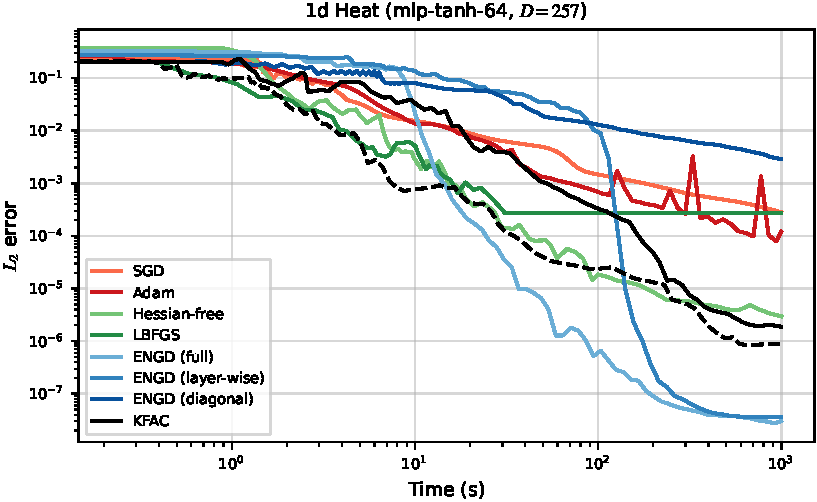
\includegraphics[trim={0 1.3cm 0 0},clip]{\pathToFigs/l2_error_over_time.pdf}
    % trim the legend and titles
    % [trim={left bottom right top},clip]
    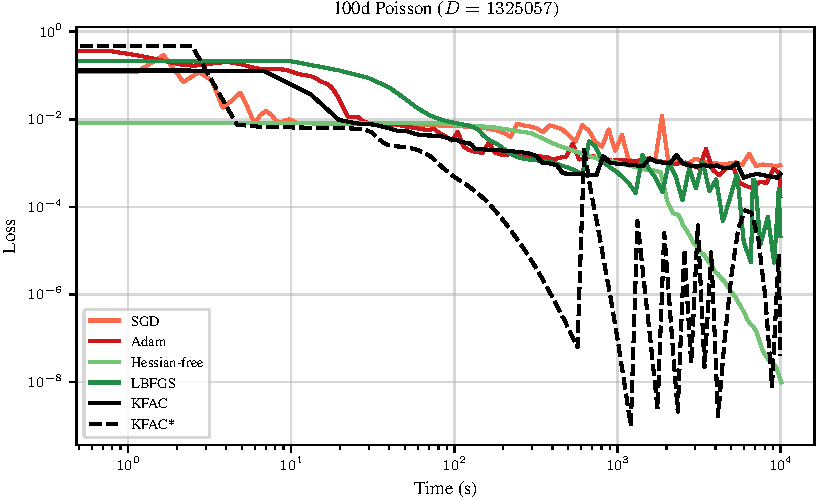
\includegraphics[trim={0 0.8cm 0 0.3cm},clip]{\pathToFigs/loss_over_time.pdf}
  \end{subfigure}
  \begin{subfigure}[t]{1.0\linewidth}
    \caption{}\label{subfig:poisson2d-step}
    % trim the legend, xlabel and xticklabels
    % [trim={left bottom right top},clip]
    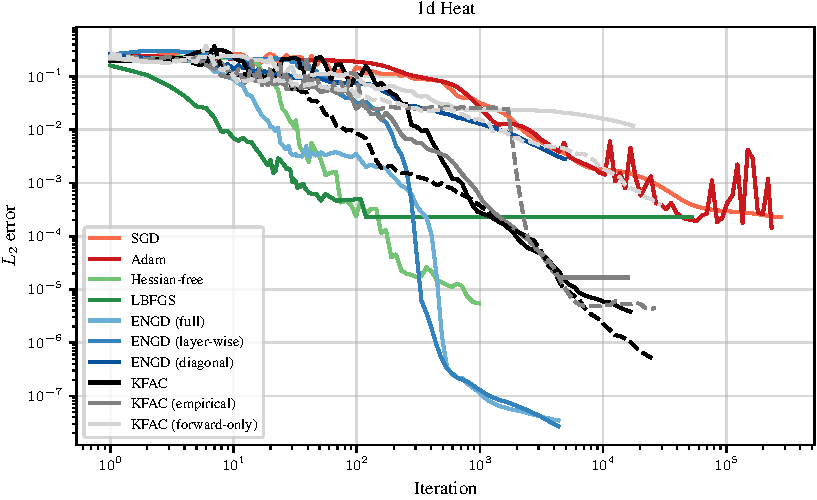
\includegraphics[trim={0 1.3cm 0 0.3cm},clip]{\pathToFigs/l2_error_over_step.pdf}
    % trim the titles
    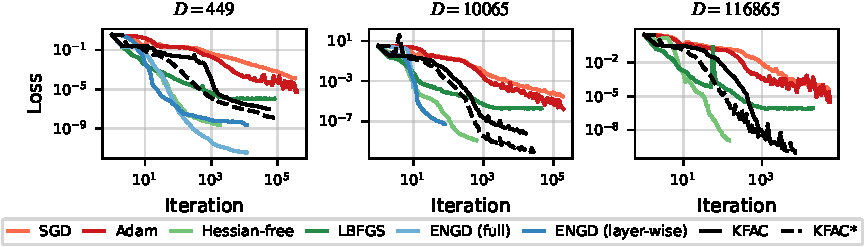
\includegraphics[trim={0 0 0 0.3cm},clip]{\pathToFigs/loss_over_step.pdf}
  \end{subfigure}
  \caption{ Training loss and evaluation $L_2$ error for learning the solution to a 2d Poisson equation over (\subref{subfig:poisson2d-time}) time and (\subref{subfig:poisson2d-step}) steps.
    Columns are different neural networks.}\label{fig:poisson2d-appendix}
\end{figure}

\begin{table}[!h]
  \centering
  \def\pathToRuns{kfac_pinns_exp/exp42_visualize_solutions/visualize_solution}
  \renewcommand\tabularxcolumn[1]{>{\Centering}m{#1}}
  \begin{small}
    \begin{tabularx}{\textwidth}{XXXXXX}
      \textbf{Optimizer} & \textbf{First step} & \textbf{0.1\% trained} & \textbf{1\% trained} & \textbf{10\% trained} & \textbf{True solution}
      \\
      SGD
      % [trim={left bottom right top},clip]
      &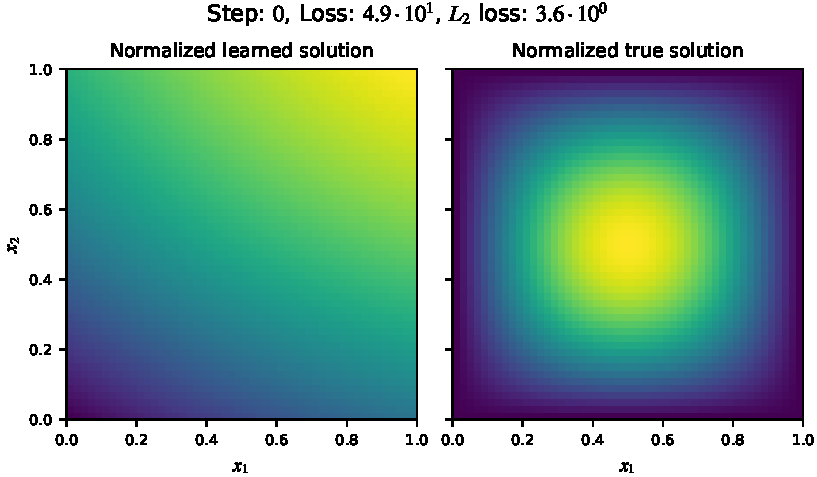
\includegraphics[trim={0.9cm 0.8cm 6.5cm 1.0cm},clip,scale=0.31]{\pathToRuns/SGD/poisson_2d_sin_product_mlp-tanh-64_SGD_step0000000.pdf}
      &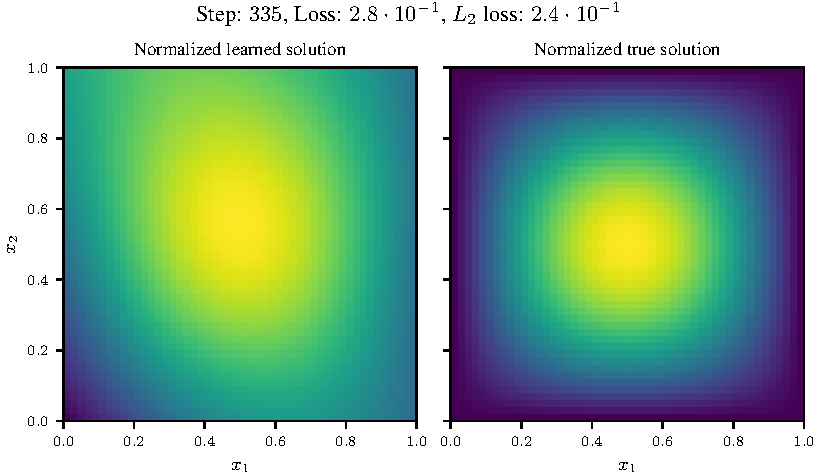
\includegraphics[trim={0.9cm 0.8cm 6.5cm 1.0cm},clip,scale=0.31]{\pathToRuns/SGD/poisson_2d_sin_product_mlp-tanh-64_SGD_step0000335.pdf}
      &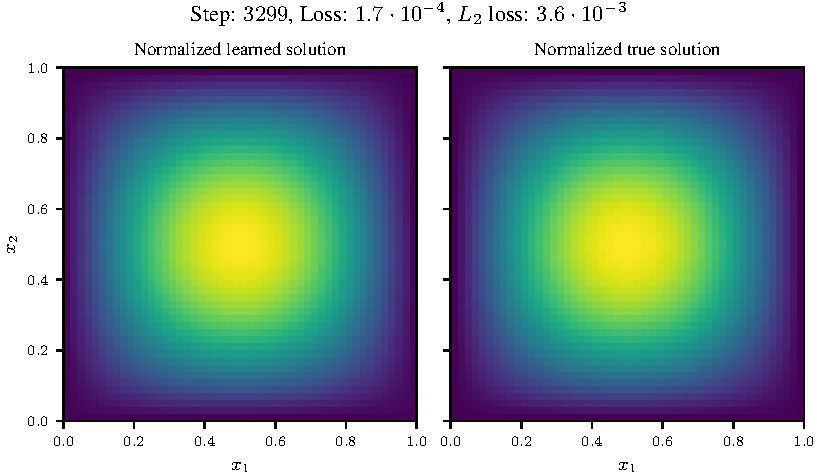
\includegraphics[trim={0.9cm 0.8cm 6.5cm 1.0cm},clip,scale=0.31]{\pathToRuns/SGD/poisson_2d_sin_product_mlp-tanh-64_SGD_step0003299.pdf}
      &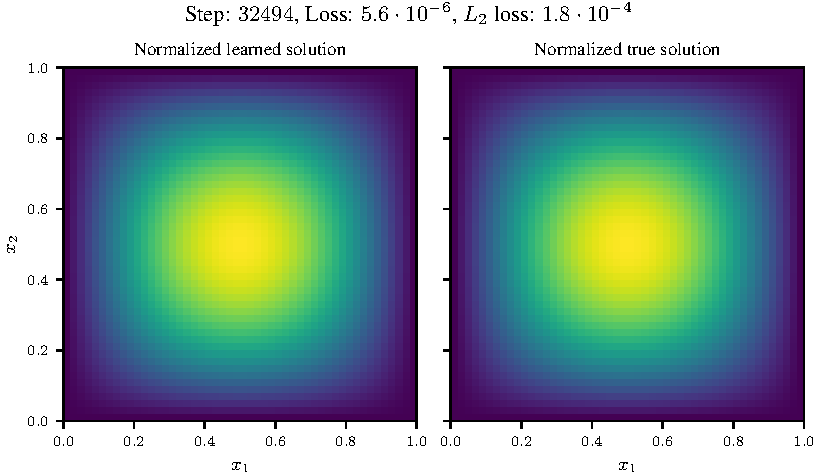
\includegraphics[trim={0.9cm 0.8cm 6.5cm 1.0cm},clip,scale=0.31]{\pathToRuns/SGD/poisson_2d_sin_product_mlp-tanh-64_SGD_step0032494.pdf}
      &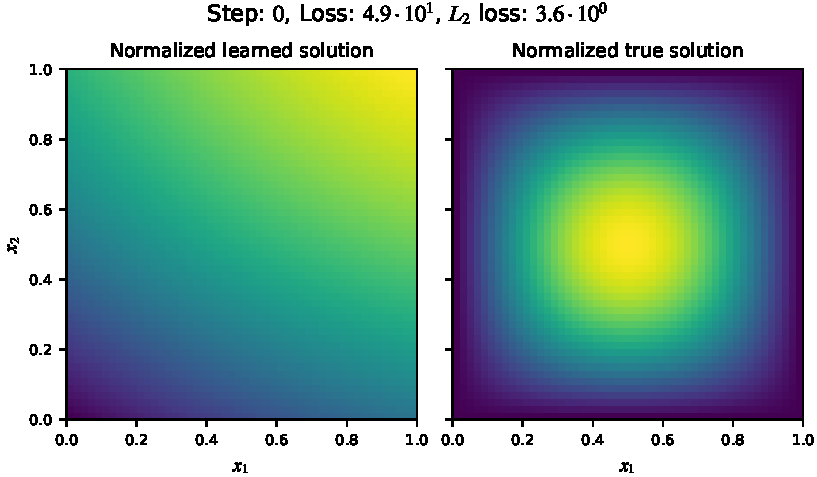
\includegraphics[trim={7.25cm 0.8cm 0 1.0cm},clip,scale=0.31]{\pathToRuns/SGD/poisson_2d_sin_product_mlp-tanh-64_SGD_step0000000.pdf}
      \\
      Adam
      % [trim={left bottom right top},clip]
      &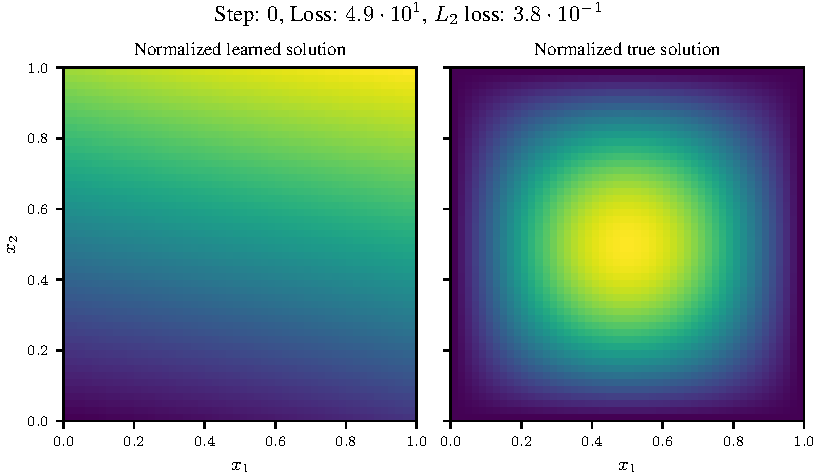
\includegraphics[trim={0.9cm 0.8cm 6.5cm 1.0cm},clip,scale=0.31]{\pathToRuns/Adam/poisson_2d_sin_product_mlp-tanh-64_Adam_step0000000.pdf}
      &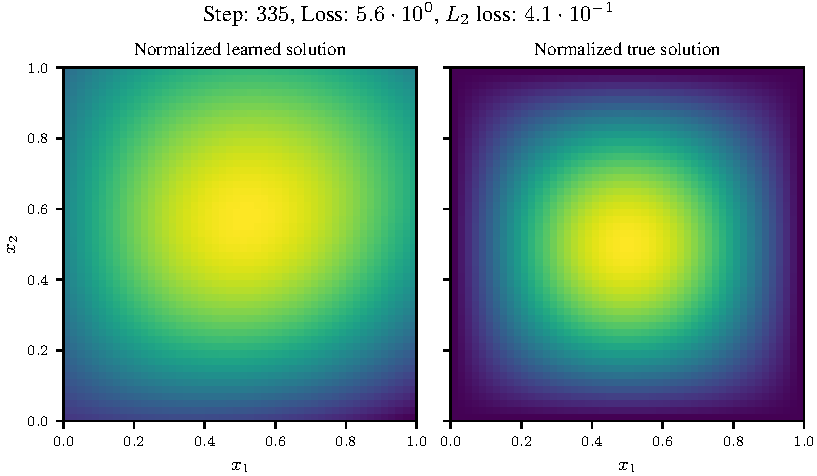
\includegraphics[trim={0.9cm 0.8cm 6.5cm 1.0cm},clip,scale=0.31]{\pathToRuns/Adam/poisson_2d_sin_product_mlp-tanh-64_Adam_step0000335.pdf}
      &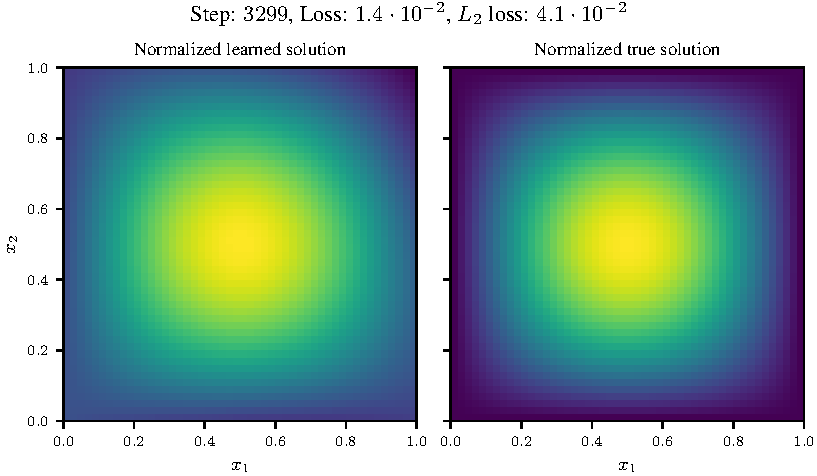
\includegraphics[trim={0.9cm 0.8cm 6.5cm 1.0cm},clip,scale=0.31]{\pathToRuns/Adam/poisson_2d_sin_product_mlp-tanh-64_Adam_step0003299.pdf}
      &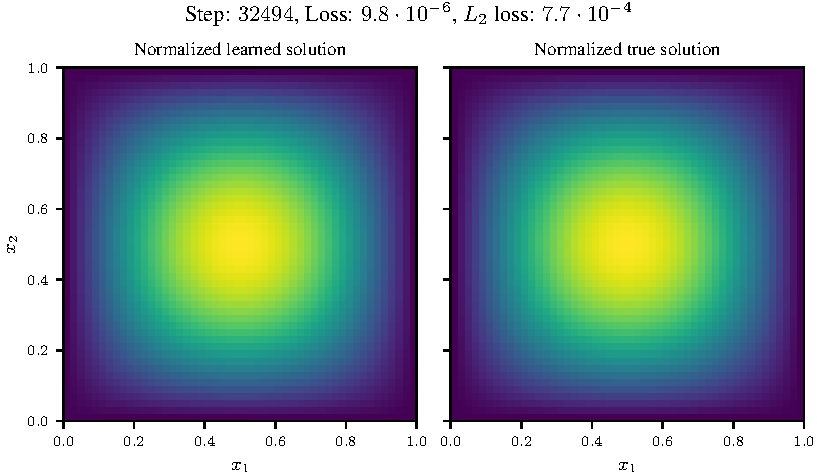
\includegraphics[trim={0.9cm 0.8cm 6.5cm 1.0cm},clip,scale=0.31]{\pathToRuns/Adam/poisson_2d_sin_product_mlp-tanh-64_Adam_step0032494.pdf}
      &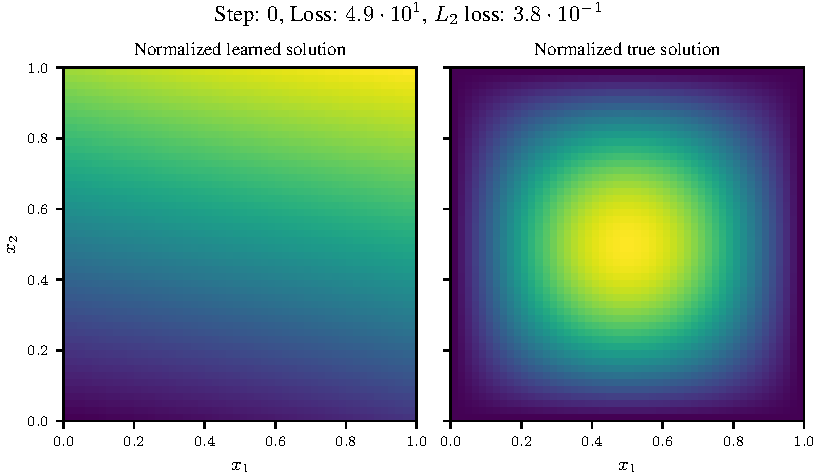
\includegraphics[trim={7.25cm 0.8cm 0 1.0cm},clip,scale=0.31]{\pathToRuns/Adam/poisson_2d_sin_product_mlp-tanh-64_Adam_step0000000.pdf}
      \\
      % [trim={left bottom right top},clip]
      LBFGS
      & 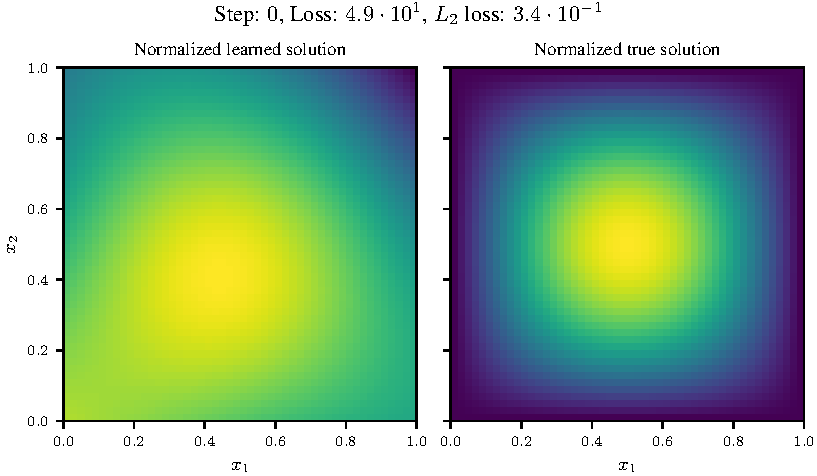
\includegraphics[trim={0.9cm 0.8cm 6.5cm 1.0cm},clip,scale=0.31]{\pathToRuns/LBFGS/poisson_2d_sin_product_mlp-tanh-64_LBFGS_step0000000.pdf}
      & 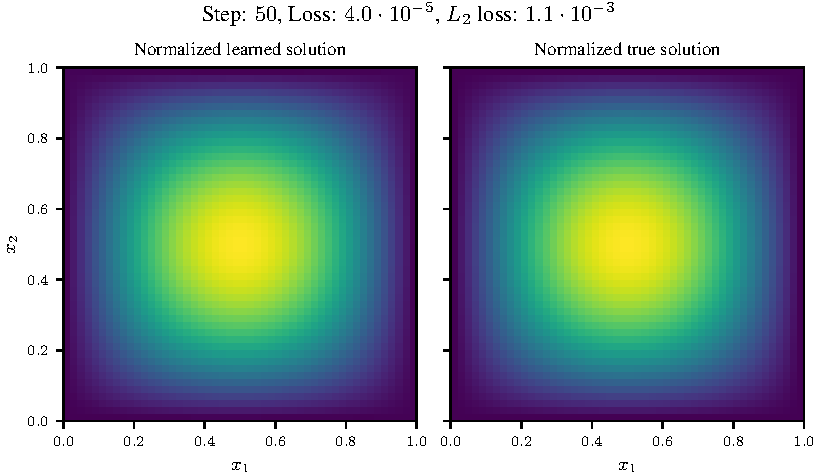
\includegraphics[trim={0.9cm 0.8cm 6.5cm 1.0cm},clip,scale=0.31]{\pathToRuns/LBFGS/poisson_2d_sin_product_mlp-tanh-64_LBFGS_step0000050.pdf}
      & 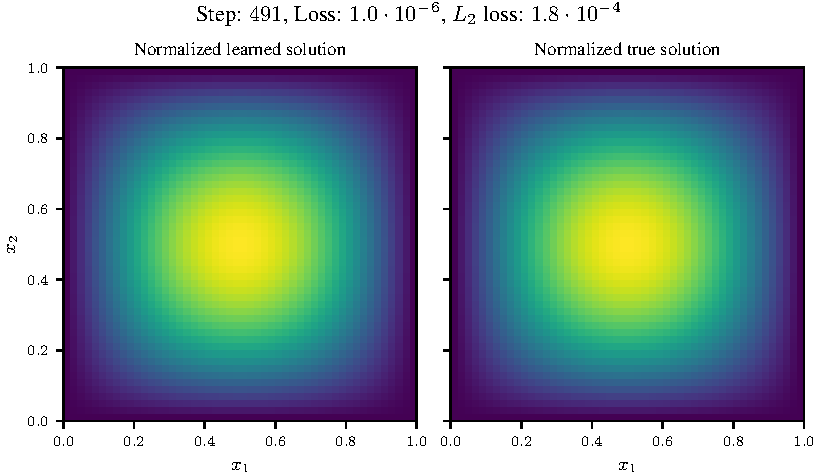
\includegraphics[trim={0.9cm 0.8cm 6.5cm 1.0cm},clip,scale=0.31]{\pathToRuns/LBFGS/poisson_2d_sin_product_mlp-tanh-64_LBFGS_step0000491.pdf}
      & 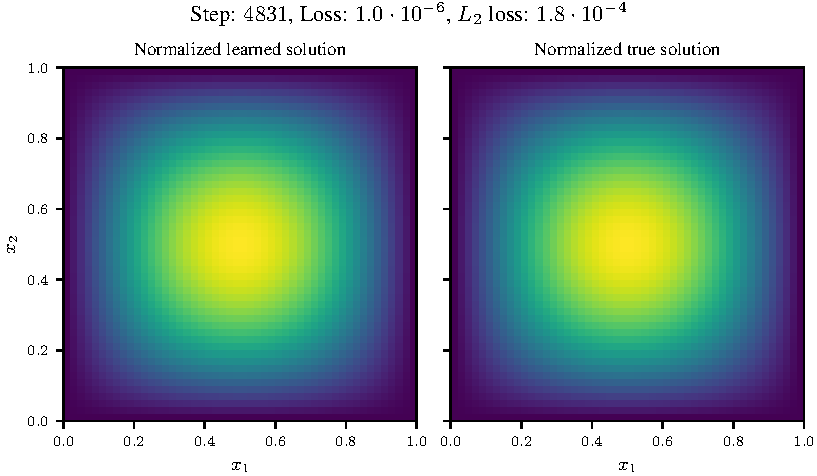
\includegraphics[trim={0.9cm 0.8cm 6.5cm 1.0cm},clip,scale=0.31]{\pathToRuns/LBFGS/poisson_2d_sin_product_mlp-tanh-64_LBFGS_step0004831.pdf}
      & 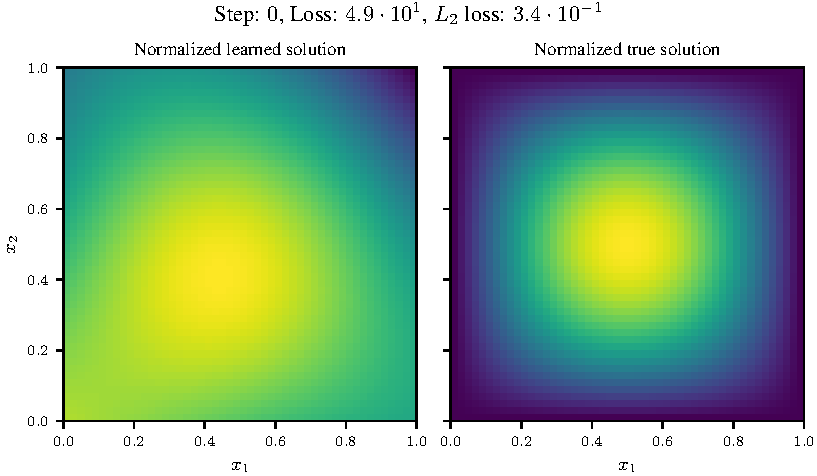
\includegraphics[trim={7.25cm 0.8cm 0 1.0cm},clip,scale=0.31]{\pathToRuns/LBFGS/poisson_2d_sin_product_mlp-tanh-64_LBFGS_step0000000.pdf}
      \\
      Hessian-free
      % [trim={left bottom right top},clip]
      &\includegraphics[trim={0.9cm 0.8cm 6.5cm 1.0cm},clip,scale=0.31]{\pathToRuns/Hessian-free/poisson_2d_sin_product_mlp-tanh-64_Hessianfree_step0000000.pdf}
      &\includegraphics[trim={0.9cm 0.8cm 6.5cm 1.0cm},clip,scale=0.31]{\pathToRuns/Hessian-free/poisson_2d_sin_product_mlp-tanh-64_Hessianfree_step0000004.pdf}
      &\includegraphics[trim={0.9cm 0.8cm 6.5cm 1.0cm},clip,scale=0.31]{\pathToRuns/Hessian-free/poisson_2d_sin_product_mlp-tanh-64_Hessianfree_step0000035.pdf}
      &\includegraphics[trim={0.9cm 0.8cm 6.5cm 1.0cm},clip,scale=0.31]{\pathToRuns/Hessian-free/poisson_2d_sin_product_mlp-tanh-64_Hessianfree_step0000335.pdf}
      &\includegraphics[trim={7.25cm 0.8cm 0 1.0cm},clip,scale=0.31]{\pathToRuns/Hessian-free/poisson_2d_sin_product_mlp-tanh-64_Hessianfree_step0000000.pdf}
      \\
      % [trim={left bottom right top},clip]
      ENGD (full)
      &\includegraphics[trim={0.9cm 0.8cm 6.5cm 1.0cm},clip,scale=0.31]{\pathToRuns/ENGD_full/poisson_2d_sin_product_mlp-tanh-64_ENGD_step0000000.pdf}
      &\includegraphics[trim={0.9cm 0.8cm 6.5cm 1.0cm},clip,scale=0.31]{\pathToRuns/ENGD_full/poisson_2d_sin_product_mlp-tanh-64_ENGD_step0000006.pdf}
      &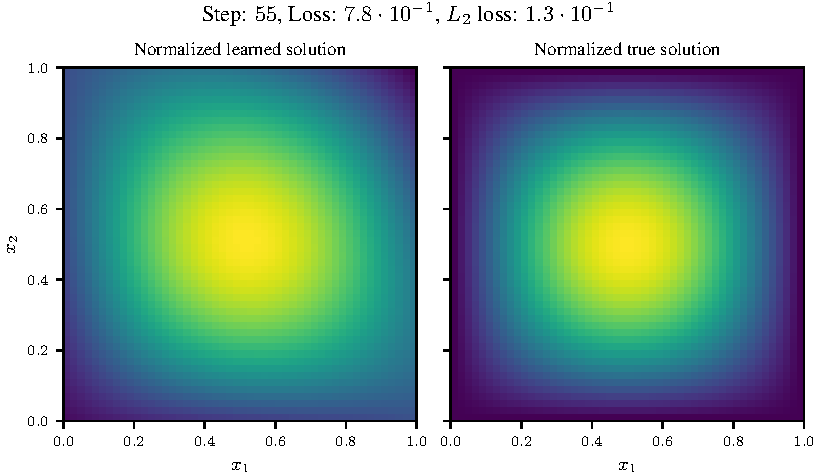
\includegraphics[trim={0.9cm 0.8cm 6.5cm 1.0cm},clip,scale=0.31]{\pathToRuns/ENGD_full/poisson_2d_sin_product_mlp-tanh-64_ENGD_step0000055.pdf}
      &\includegraphics[trim={0.9cm 0.8cm 6.5cm 1.0cm},clip,scale=0.31]{\pathToRuns/ENGD_full/poisson_2d_sin_product_mlp-tanh-64_ENGD_step0000594.pdf}
      &\includegraphics[trim={7.25cm 0.8cm 0 1.0cm},clip,scale=0.31]{\pathToRuns/ENGD_full/poisson_2d_sin_product_mlp-tanh-64_ENGD_step0000000.pdf}
      \\
      ENGD (layer-wise)
      % [trim={left bottom right top},clip]
      &\includegraphics[trim={0.9cm 0.8cm 6.5cm 1.0cm},clip,scale=0.31]{\pathToRuns/ENGD_layer-wise/poisson_2d_sin_product_mlp-tanh-64_ENGD_step0000000.pdf}
      &\includegraphics[trim={0.9cm 0.8cm 6.5cm 1.0cm},clip,scale=0.31]{\pathToRuns/ENGD_layer-wise/poisson_2d_sin_product_mlp-tanh-64_ENGD_step0000006.pdf}
      &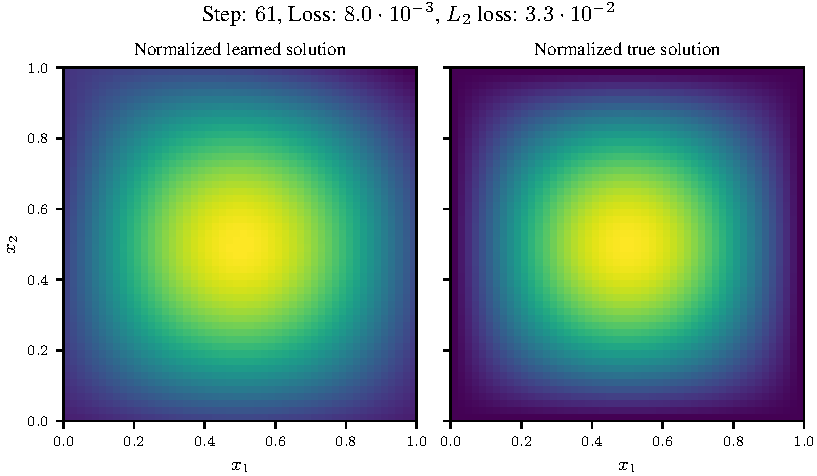
\includegraphics[trim={0.9cm 0.8cm 6.5cm 1.0cm},clip,scale=0.31]{\pathToRuns/ENGD_layer-wise/poisson_2d_sin_product_mlp-tanh-64_ENGD_step0000061.pdf}
      &\includegraphics[trim={0.9cm 0.8cm 6.5cm 1.0cm},clip,scale=0.31]{\pathToRuns/ENGD_layer-wise/poisson_2d_sin_product_mlp-tanh-64_ENGD_step0000594.pdf}
      &\includegraphics[trim={7.25cm 0.8cm 0 1.0cm},clip,scale=0.31]{\pathToRuns/ENGD_layer-wise/poisson_2d_sin_product_mlp-tanh-64_ENGD_step0000000.pdf}
      \\
      KFAC
      % [trim={left bottom right top},clip]
      &\includegraphics[trim={0.9cm 0.8cm 6.5cm 1.0cm},clip,scale=0.31]{\pathToRuns/KFAC/poisson_2d_sin_product_mlp-tanh-64_KFAC_step0000000.pdf}
      &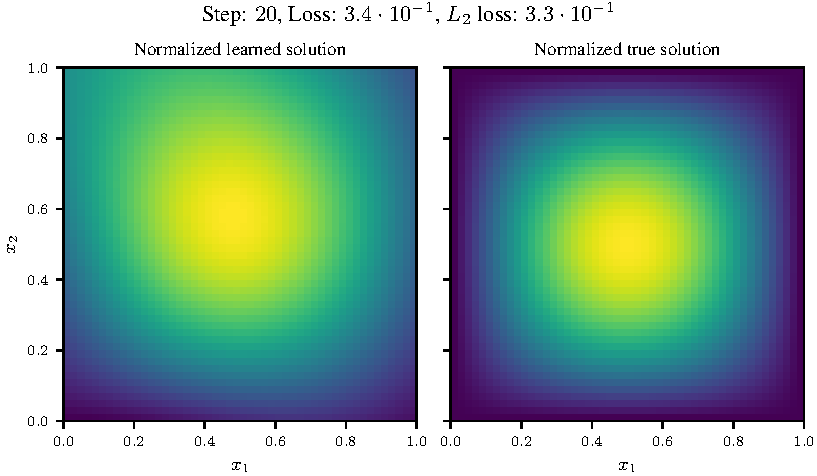
\includegraphics[trim={0.9cm 0.8cm 6.5cm 1.0cm},clip,scale=0.31]{\pathToRuns/KFAC/poisson_2d_sin_product_mlp-tanh-64_KFAC_step0000020.pdf}
      &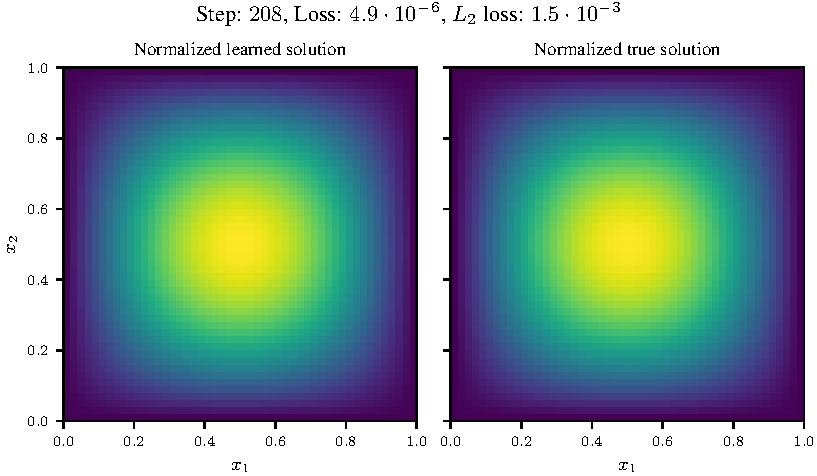
\includegraphics[trim={0.9cm 0.8cm 6.5cm 1.0cm},clip,scale=0.31]{\pathToRuns/KFAC/poisson_2d_sin_product_mlp-tanh-64_KFAC_step0000208.pdf}
      &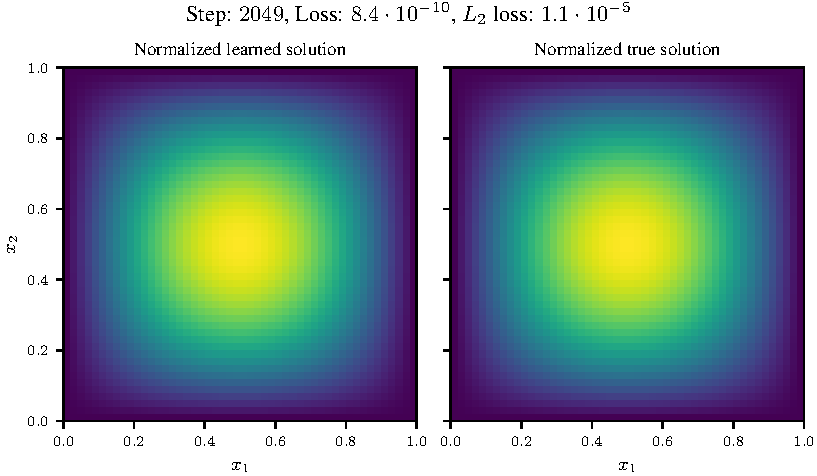
\includegraphics[trim={0.9cm 0.8cm 6.5cm 1.0cm},clip,scale=0.31]{\pathToRuns/KFAC/poisson_2d_sin_product_mlp-tanh-64_KFAC_step0002049.pdf}
      &\includegraphics[trim={7.25cm 0.8cm 0 1.0cm},clip,scale=0.31]{\pathToRuns/KFAC/poisson_2d_sin_product_mlp-tanh-64_KFAC_step0000000.pdf}
      \\
      KFAC*
      % [trim={left bottom right top},clip]
      &\includegraphics[trim={0.9cm 0.8cm 6.5cm 1.0cm},clip,scale=0.31]{\pathToRuns/KFAC_auto/poisson_2d_sin_product_mlp-tanh-64_KFAC_step0000000.pdf}
      &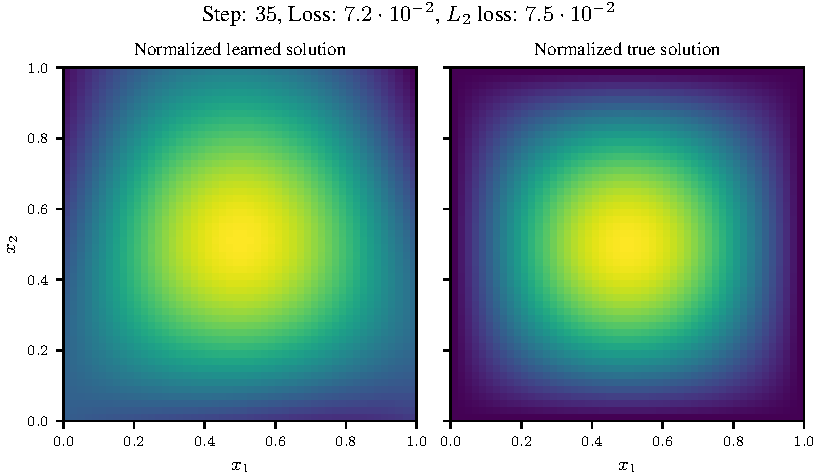
\includegraphics[trim={0.9cm 0.8cm 6.5cm 1.0cm},clip,scale=0.31]{\pathToRuns/KFAC_auto/poisson_2d_sin_product_mlp-tanh-64_KFAC_step0000035.pdf}
      &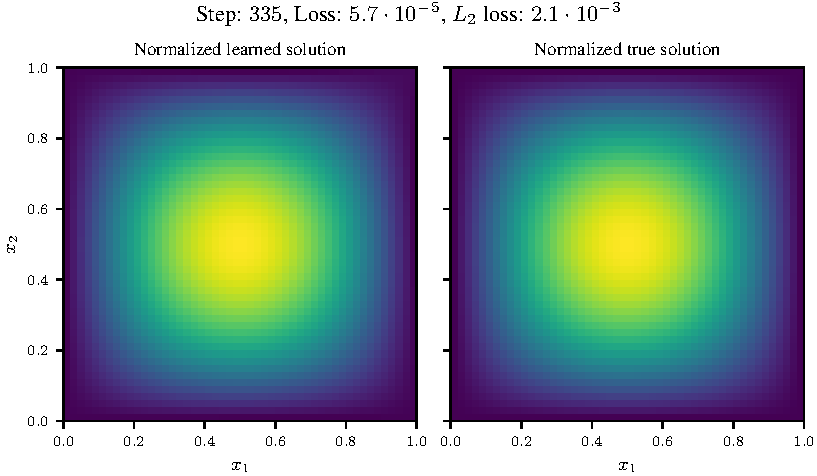
\includegraphics[trim={0.9cm 0.8cm 6.5cm 1.0cm},clip,scale=0.31]{\pathToRuns/KFAC_auto/poisson_2d_sin_product_mlp-tanh-64_KFAC_step0000335.pdf}
      &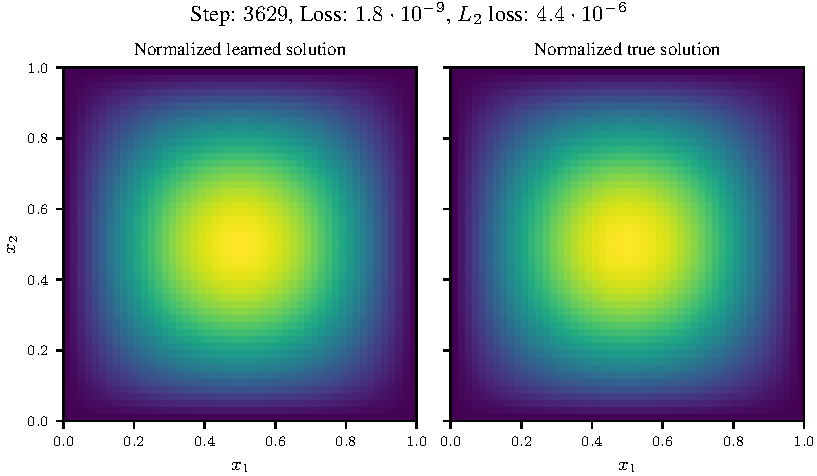
\includegraphics[trim={0.9cm 0.8cm 6.5cm 1.0cm},clip,scale=0.31]{\pathToRuns/KFAC_auto/poisson_2d_sin_product_mlp-tanh-64_KFAC_step0003629.pdf}
      &\includegraphics[trim={7.25cm 0.8cm 0 1.0cm},clip,scale=0.31]{\pathToRuns/KFAC_auto/poisson_2d_sin_product_mlp-tanh-64_KFAC_step0000000.pdf}
    \end{tabularx}
  \end{small}
  \captionof{figure}{Visual comparison learned and true solutions while training with different optimizers for the 2d Poisson equation using a two-layer MLP (corresponding to the curves in \Cref{fig:2D-Poisson} left).
    All functions are shown on the unit square $(x, y) \in \Omega = [0; 1]^2$ and normalized to the unit interval.}
  \label{fig:2d-poisson-visualization}
\end{table}

\paragraph{Best run details}
The runs shown in \Cref{fig:poisson2d-appendix} correspond to the following hyper-parameters:
\begin{itemize}
\item $2\to 64\to 1$ MLP with $D=257$
  \begin{itemize}
    \def\pathToRuns{kfac_pinns_exp/exp09_reproduce_poisson2d/tex}
  \item \textbf{SGD:} learning rate: $\num[scientific-notation=true]{1.007555e-03}$, momentum: $\num[scientific-notation=true]{0.9}$
  \item \textbf{Adam:} learning rate: $\num[scientific-notation=true]{1.369294e-06}$, $N_{\Omega}$: $\num[scientific-notation=false]{203}$, $N_{\partial\Omega}$: $\num[scientific-notation=false]{1494}$, batch sampling frequency: $\num[scientific-notation=false]{9712}$
  \item \textbf{Hessian-free:} curvature matrix: $\text{GGN}$, initial damping: $\num[scientific-notation=true]{1.146081e-02}$, constant damping: $\text{no}$, maximum CG iterations: $\num[scientific-notation=false]{484}$, $N_{\Omega}$: $\num[scientific-notation=false]{2410}$, $N_{\partial\Omega}$: $\num[scientific-notation=false]{2448}$, batch sampling frequency: $\num[scientific-notation=false]{1311}$
  \item \textbf{LBFGS:} learning rate: $\num[scientific-notation=true]{0.2}$, history size: $\num[scientific-notation=false]{225}$
  \item \textbf{ENGD (full):} damping: $\num[scientific-notation=true]{1e-10}$, exponential moving average: $\num[scientific-notation=true]{0.3}$, initialize Gramian to identity: $\text{yes}$
  \item \textbf{ENGD (layer-wise):} damping: $\num[scientific-notation=true]{1e-06}$, exponential moving average: $\num[scientific-notation=true]{0.3}$, initialize Gramian to identity: $\text{no}$
  \item \textbf{KFAC:} damping: $\num[scientific-notation=true]{8.435180e-14}$, momentum: $\num[scientific-notation=true]{9.718645e-01}$, exponential moving average: $\num[scientific-notation=true]{9.800744e-01}$, initialize Kronecker factors to identity: $\text{yes}$, $N_{\Omega}$: $\num[scientific-notation=false]{2525}$, $N_{\partial\Omega}$: $\num[scientific-notation=false]{2663}$, batch sampling frequency: $\num[scientific-notation=false]{7916}$
  \item \textbf{KFAC*:} damping: $\num[scientific-notation=true]{2.965060e-08}$, exponential moving average: $\num[scientific-notation=true]{9.574717e-01}$, initialize Kronecker factors to identity: $\text{yes}$
  \end{itemize}

\item $2 \to 64 \to 64 \to 48 \to 48 \to 1$ MLP with $D=\num{9873}$
  \begin{itemize}
    \def\pathToRuns{kfac_pinns_exp/exp15_poisson2d_deepwide/tex}
  \item \textbf{SGD:} learning rate: $\num[scientific-notation=true]{1.007555e-03}$, momentum: $\num[scientific-notation=true]{0.9}$
  \item \textbf{Adam:} learning rate: $\num[scientific-notation=true]{1.369294e-06}$, $N_{\Omega}$: $\num[scientific-notation=false]{203}$, $N_{\partial\Omega}$: $\num[scientific-notation=false]{1494}$, batch sampling frequency: $\num[scientific-notation=false]{9712}$
  \item \textbf{Hessian-free:} curvature matrix: $\text{GGN}$, initial damping: $\num[scientific-notation=true]{1.146081e-02}$, constant damping: $\text{no}$, maximum CG iterations: $\num[scientific-notation=false]{484}$, $N_{\Omega}$: $\num[scientific-notation=false]{2410}$, $N_{\partial\Omega}$: $\num[scientific-notation=false]{2448}$, batch sampling frequency: $\num[scientific-notation=false]{1311}$
  \item \textbf{LBFGS:} learning rate: $\num[scientific-notation=true]{0.2}$, history size: $\num[scientific-notation=false]{225}$
  \item \textbf{ENGD (full):} damping: $\num[scientific-notation=true]{1e-10}$, exponential moving average: $\num[scientific-notation=true]{0.3}$, initialize Gramian to identity: $\text{yes}$
  \item \textbf{ENGD (layer-wise):} damping: $\num[scientific-notation=true]{1e-06}$, exponential moving average: $\num[scientific-notation=true]{0.3}$, initialize Gramian to identity: $\text{no}$
  \item \textbf{KFAC:} damping: $\num[scientific-notation=true]{8.435180e-14}$, momentum: $\num[scientific-notation=true]{9.718645e-01}$, exponential moving average: $\num[scientific-notation=true]{9.800744e-01}$, initialize Kronecker factors to identity: $\text{yes}$, $N_{\Omega}$: $\num[scientific-notation=false]{2525}$, $N_{\partial\Omega}$: $\num[scientific-notation=false]{2663}$, batch sampling frequency: $\num[scientific-notation=false]{7916}$
  \item \textbf{KFAC*:} damping: $\num[scientific-notation=true]{2.965060e-08}$, exponential moving average: $\num[scientific-notation=true]{9.574717e-01}$, initialize Kronecker factors to identity: $\text{yes}$
  \end{itemize}

\item $2 \to 256 \to 256\to 128 \to 128 \to 1$ MLP with $D=\num{116097}$
  \begin{itemize}
    \def\pathToRuns{kfac_pinns_exp/exp20_poisson2d_mlp_tanh_256/tex}
  \item \textbf{SGD:} learning rate: $\num[scientific-notation=true]{1.007555e-03}$, momentum: $\num[scientific-notation=true]{0.9}$
  \item \textbf{Adam:} learning rate: $\num[scientific-notation=true]{1.369294e-06}$, $N_{\Omega}$: $\num[scientific-notation=false]{203}$, $N_{\partial\Omega}$: $\num[scientific-notation=false]{1494}$, batch sampling frequency: $\num[scientific-notation=false]{9712}$
  \item \textbf{Hessian-free:} curvature matrix: $\text{GGN}$, initial damping: $\num[scientific-notation=true]{1.146081e-02}$, constant damping: $\text{no}$, maximum CG iterations: $\num[scientific-notation=false]{484}$, $N_{\Omega}$: $\num[scientific-notation=false]{2410}$, $N_{\partial\Omega}$: $\num[scientific-notation=false]{2448}$, batch sampling frequency: $\num[scientific-notation=false]{1311}$
  \item \textbf{LBFGS:} learning rate: $\num[scientific-notation=true]{0.2}$, history size: $\num[scientific-notation=false]{225}$
  \item \textbf{KFAC:} damping: $\num[scientific-notation=true]{8.435180e-14}$, momentum: $\num[scientific-notation=true]{9.718645e-01}$, exponential moving average: $\num[scientific-notation=true]{9.800744e-01}$, initialize Kronecker factors to identity: $\text{yes}$, $N_{\Omega}$: $\num[scientific-notation=false]{2525}$, $N_{\partial\Omega}$: $\num[scientific-notation=false]{2663}$, batch sampling frequency: $\num[scientific-notation=false]{7916}$
  \item \textbf{KFAC*:} damping: $\num[scientific-notation=true]{2.965060e-08}$, exponential moving average: $\num[scientific-notation=true]{9.574717e-01}$, initialize Kronecker factors to identity: $\text{yes}$
  \end{itemize}
\end{itemize}

\paragraph{Search space details} The runs shown in \Cref{fig:poisson2d-appendix} were determined to be the best via a search with approximately 50 runs on the following search spaces which were obtained by refining an initially wider search ($\mathcal{U}$ denotes a uniform, and $\mathcal{LU}$ a log-uniform distribution):
\begin{itemize}
\item $2\to 64\to 1$ MLP with $D=257$
  \begin{itemize}
    \def\pathToRuns{kfac_pinns_exp/exp09_reproduce_poisson2d/tex}
  \item \textbf{SGD:} learning rate: $\mathcal{LU}([\num[scientific-notation=true]{1e-06}; \num[scientific-notation=false]{1}])$, momentum: $\mathcal{U}([\num[scientific-notation=false]{0}; \num[scientific-notation=true]{0.99}])$, $N_{\Omega}$: $\mathcal{C}(\{\num[scientific-notation=false]{100},\num[scientific-notation=false]{101},\text{\dots},\num[scientific-notation=false]{5000}\})$, $N_{\partial\Omega}$: $\mathcal{C}(\{\num[scientific-notation=false]{50},\num[scientific-notation=false]{51},\text{\dots},\num[scientific-notation=false]{2500}\})$, batch sampling frequency: $\mathcal{C}(\{\num[scientific-notation=false]{0},\num[scientific-notation=false]{1},\text{\dots},\num[scientific-notation=false]{1000}\})$
  \item \textbf{Adam:} learning rate: $\mathcal{LU}([\num[scientific-notation=true]{0.0001}; \num[scientific-notation=true]{0.5}])$
  \item \textbf{Hessian-free:} curvature matrix: $\mathcal{U}(\{\text{GGN},\text{Hessian}\})$, initial damping: $\mathcal{LU}([\num[scientific-notation=true]{1e-15}; \num[scientific-notation=false]{1}])$, constant damping: $\mathcal{U}(\{\text{no},\text{yes}\})$, maximum CG iterations: $\mathcal{U}(\{\num[scientific-notation=false]{1},\num[scientific-notation=false]{2},\text{\dots},\num[scientific-notation=false]{500}\})$, $N_{\Omega}$: $\mathcal{U}(\{\num[scientific-notation=false]{100},\num[scientific-notation=false]{101},\text{\dots},\num[scientific-notation=false]{5000}\})$, $N_{\partial\Omega}$: $\mathcal{U}(\{\num[scientific-notation=false]{50},\num[scientific-notation=false]{51},\text{\dots},\num[scientific-notation=false]{2500}\})$, batch sampling frequency: $\mathcal{U}(\{\num[scientific-notation=false]{0},\num[scientific-notation=false]{1},\text{\dots},\num[scientific-notation=false]{5000}\})$
  \item \textbf{LBFGS:} learning rate: $\mathcal{C}(\{\num[scientific-notation=true]{0.5},\num[scientific-notation=true]{0.2},\num[scientific-notation=true]{0.1},\num[scientific-notation=true]{0.05},\num[scientific-notation=true]{0.02},\num[scientific-notation=true]{0.01}\})$, history size: $\mathcal{C}(\{\num[scientific-notation=false]{75},\num[scientific-notation=false]{100},\num[scientific-notation=false]{125},\num[scientific-notation=false]{150},\num[scientific-notation=false]{175},\num[scientific-notation=false]{200},\num[scientific-notation=false]{225},\num[scientific-notation=false]{250}\})$
  \item \textbf{ENGD (full):} damping: $\mathcal{C}(\{\num[scientific-notation=true]{1e-08},\num[scientific-notation=true]{1e-09},\num[scientific-notation=true]{1e-10},\num[scientific-notation=true]{1e-11},\num[scientific-notation=true]{1e-12},\num[scientific-notation=false]{0}\})$, exponential moving average: $\mathcal{C}(\{\num[scientific-notation=false]{0},\num[scientific-notation=true]{0.3},\num[scientific-notation=true]{0.6},\num[scientific-notation=true]{0.9}\})$, initialize Gramian to identity: $\mathcal{C}(\{\text{no},\text{yes}\})$
  \item \textbf{ENGD (layer-wise):} damping: $\mathcal{U}(\{\num[scientific-notation=true]{0.01},\num[scientific-notation=true]{0.001},\num[scientific-notation=true]{0.0001},\num[scientific-notation=true]{1e-05},\num[scientific-notation=true]{1e-06}\})$, exponential moving average: $\mathcal{U}(\{\num[scientific-notation=false]{0},\num[scientific-notation=true]{0.3},\num[scientific-notation=true]{0.6},\num[scientific-notation=true]{0.9},\num[scientific-notation=true]{0.99}\})$, initialize Gramian to identity: $\mathcal{U}(\{\text{no},\text{yes}\})$
  \item \textbf{KFAC:} damping: $\mathcal{LU}([\num[scientific-notation=true]{1e-15}; \num[scientific-notation=true]{0.01}])$, momentum: $\mathcal{U}([\num[scientific-notation=false]{0}; \num[scientific-notation=true]{0.99}])$, exponential moving average: $\mathcal{U}([\num[scientific-notation=false]{0}; \num[scientific-notation=true]{0.99}])$, initialize Kronecker factors to identity: $\mathcal{C}(\{\text{no},\text{yes}\})$
  \item \textbf{KFAC*:} damping: $\mathcal{LU}([\num[scientific-notation=true]{1e-15}; \num[scientific-notation=true]{0.01}])$, exponential moving average: $\mathcal{U}([\num[scientific-notation=false]{0}; \num[scientific-notation=true]{0.99}])$, initialize Kronecker factors to identity: $\mathcal{U}(\{\text{no},\text{yes}\})$, $N_{\Omega}$: $\mathcal{U}(\{\num[scientific-notation=false]{100},\num[scientific-notation=false]{101},\text{\dots},\num[scientific-notation=false]{5000}\})$, $N_{\partial\Omega}$: $\mathcal{U}(\{\num[scientific-notation=false]{50},\num[scientific-notation=false]{51},\text{\dots},\num[scientific-notation=false]{2500}\})$, batch sampling frequency: $\mathcal{U}(\{\num[scientific-notation=false]{0},\num[scientific-notation=false]{1},\text{\dots},\num[scientific-notation=false]{5000}\})$
  \end{itemize}

\item $2 \to 64 \to 64 \to 48 \to 48 \to 1$ MLP with $D=\num{9873}$
  \begin{itemize}
    \def\pathToRuns{kfac_pinns_exp/exp15_poisson2d_deepwide/tex}
  \item \textbf{SGD:} learning rate: $\mathcal{LU}([\num[scientific-notation=true]{1e-06}; \num[scientific-notation=false]{1}])$, momentum: $\mathcal{U}([\num[scientific-notation=false]{0}; \num[scientific-notation=true]{0.99}])$, $N_{\Omega}$: $\mathcal{C}(\{\num[scientific-notation=false]{100},\num[scientific-notation=false]{101},\text{\dots},\num[scientific-notation=false]{5000}\})$, $N_{\partial\Omega}$: $\mathcal{C}(\{\num[scientific-notation=false]{50},\num[scientific-notation=false]{51},\text{\dots},\num[scientific-notation=false]{2500}\})$, batch sampling frequency: $\mathcal{C}(\{\num[scientific-notation=false]{0},\num[scientific-notation=false]{1},\text{\dots},\num[scientific-notation=false]{1000}\})$
  \item \textbf{Adam:} learning rate: $\mathcal{LU}([\num[scientific-notation=true]{0.0001}; \num[scientific-notation=true]{0.5}])$
  \item \textbf{Hessian-free:} curvature matrix: $\mathcal{U}(\{\text{GGN},\text{Hessian}\})$, initial damping: $\mathcal{LU}([\num[scientific-notation=true]{1e-15}; \num[scientific-notation=false]{1}])$, constant damping: $\mathcal{U}(\{\text{no},\text{yes}\})$, maximum CG iterations: $\mathcal{U}(\{\num[scientific-notation=false]{1},\num[scientific-notation=false]{2},\text{\dots},\num[scientific-notation=false]{500}\})$, $N_{\Omega}$: $\mathcal{U}(\{\num[scientific-notation=false]{100},\num[scientific-notation=false]{101},\text{\dots},\num[scientific-notation=false]{5000}\})$, $N_{\partial\Omega}$: $\mathcal{U}(\{\num[scientific-notation=false]{50},\num[scientific-notation=false]{51},\text{\dots},\num[scientific-notation=false]{2500}\})$, batch sampling frequency: $\mathcal{U}(\{\num[scientific-notation=false]{0},\num[scientific-notation=false]{1},\text{\dots},\num[scientific-notation=false]{5000}\})$
  \item \textbf{LBFGS:} learning rate: $\mathcal{C}(\{\num[scientific-notation=true]{0.5},\num[scientific-notation=true]{0.2},\num[scientific-notation=true]{0.1},\num[scientific-notation=true]{0.05},\num[scientific-notation=true]{0.02},\num[scientific-notation=true]{0.01}\})$, history size: $\mathcal{C}(\{\num[scientific-notation=false]{75},\num[scientific-notation=false]{100},\num[scientific-notation=false]{125},\num[scientific-notation=false]{150},\num[scientific-notation=false]{175},\num[scientific-notation=false]{200},\num[scientific-notation=false]{225},\num[scientific-notation=false]{250}\})$
  \item \textbf{ENGD (full):} damping: $\mathcal{C}(\{\num[scientific-notation=true]{1e-08},\num[scientific-notation=true]{1e-09},\num[scientific-notation=true]{1e-10},\num[scientific-notation=true]{1e-11},\num[scientific-notation=true]{1e-12},\num[scientific-notation=false]{0}\})$, exponential moving average: $\mathcal{C}(\{\num[scientific-notation=false]{0},\num[scientific-notation=true]{0.3},\num[scientific-notation=true]{0.6},\num[scientific-notation=true]{0.9}\})$, initialize Gramian to identity: $\mathcal{C}(\{\text{no},\text{yes}\})$
  \item \textbf{ENGD (layer-wise):} damping: $\mathcal{U}(\{\num[scientific-notation=true]{0.01},\num[scientific-notation=true]{0.001},\num[scientific-notation=true]{0.0001},\num[scientific-notation=true]{1e-05},\num[scientific-notation=true]{1e-06}\})$, exponential moving average: $\mathcal{U}(\{\num[scientific-notation=false]{0},\num[scientific-notation=true]{0.3},\num[scientific-notation=true]{0.6},\num[scientific-notation=true]{0.9},\num[scientific-notation=true]{0.99}\})$, initialize Gramian to identity: $\mathcal{U}(\{\text{no},\text{yes}\})$
  \item \textbf{KFAC:} damping: $\mathcal{LU}([\num[scientific-notation=true]{1e-15}; \num[scientific-notation=true]{0.01}])$, momentum: $\mathcal{U}([\num[scientific-notation=false]{0}; \num[scientific-notation=true]{0.99}])$, exponential moving average: $\mathcal{U}([\num[scientific-notation=false]{0}; \num[scientific-notation=true]{0.99}])$, initialize Kronecker factors to identity: $\mathcal{C}(\{\text{no},\text{yes}\})$
  \item \textbf{KFAC*:} damping: $\mathcal{LU}([\num[scientific-notation=true]{1e-15}; \num[scientific-notation=true]{0.01}])$, exponential moving average: $\mathcal{U}([\num[scientific-notation=false]{0}; \num[scientific-notation=true]{0.99}])$, initialize Kronecker factors to identity: $\mathcal{U}(\{\text{no},\text{yes}\})$, $N_{\Omega}$: $\mathcal{U}(\{\num[scientific-notation=false]{100},\num[scientific-notation=false]{101},\text{\dots},\num[scientific-notation=false]{5000}\})$, $N_{\partial\Omega}$: $\mathcal{U}(\{\num[scientific-notation=false]{50},\num[scientific-notation=false]{51},\text{\dots},\num[scientific-notation=false]{2500}\})$, batch sampling frequency: $\mathcal{U}(\{\num[scientific-notation=false]{0},\num[scientific-notation=false]{1},\text{\dots},\num[scientific-notation=false]{5000}\})$
  \end{itemize}

\item $2 \to 256 \to 256\to 128 \to 128 \to 1$ MLP with $D=\num{116097}$
  \begin{itemize}
    \def\pathToRuns{kfac_pinns_exp/exp20_poisson2d_mlp_tanh_256/tex}
  \item \textbf{SGD:} learning rate: $\mathcal{LU}([\num[scientific-notation=true]{1e-06}; \num[scientific-notation=false]{1}])$, momentum: $\mathcal{U}([\num[scientific-notation=false]{0}; \num[scientific-notation=true]{0.99}])$, $N_{\Omega}$: $\mathcal{C}(\{\num[scientific-notation=false]{100},\num[scientific-notation=false]{101},\text{\dots},\num[scientific-notation=false]{5000}\})$, $N_{\partial\Omega}$: $\mathcal{C}(\{\num[scientific-notation=false]{50},\num[scientific-notation=false]{51},\text{\dots},\num[scientific-notation=false]{2500}\})$, batch sampling frequency: $\mathcal{C}(\{\num[scientific-notation=false]{0},\num[scientific-notation=false]{1},\text{\dots},\num[scientific-notation=false]{1000}\})$
  \item \textbf{Adam:} learning rate: $\mathcal{LU}([\num[scientific-notation=true]{0.0001}; \num[scientific-notation=true]{0.5}])$
  \item \textbf{Hessian-free:} curvature matrix: $\mathcal{U}(\{\text{GGN},\text{Hessian}\})$, initial damping: $\mathcal{LU}([\num[scientific-notation=true]{1e-15}; \num[scientific-notation=false]{1}])$, constant damping: $\mathcal{U}(\{\text{no},\text{yes}\})$, maximum CG iterations: $\mathcal{U}(\{\num[scientific-notation=false]{1},\num[scientific-notation=false]{2},\text{\dots},\num[scientific-notation=false]{500}\})$, $N_{\Omega}$: $\mathcal{U}(\{\num[scientific-notation=false]{100},\num[scientific-notation=false]{101},\text{\dots},\num[scientific-notation=false]{5000}\})$, $N_{\partial\Omega}$: $\mathcal{U}(\{\num[scientific-notation=false]{50},\num[scientific-notation=false]{51},\text{\dots},\num[scientific-notation=false]{2500}\})$, batch sampling frequency: $\mathcal{U}(\{\num[scientific-notation=false]{0},\num[scientific-notation=false]{1},\text{\dots},\num[scientific-notation=false]{5000}\})$
  \item \textbf{LBFGS:} learning rate: $\mathcal{C}(\{\num[scientific-notation=true]{0.5},\num[scientific-notation=true]{0.2},\num[scientific-notation=true]{0.1},\num[scientific-notation=true]{0.05},\num[scientific-notation=true]{0.02},\num[scientific-notation=true]{0.01}\})$, history size: $\mathcal{C}(\{\num[scientific-notation=false]{75},\num[scientific-notation=false]{100},\num[scientific-notation=false]{125},\num[scientific-notation=false]{150},\num[scientific-notation=false]{175},\num[scientific-notation=false]{200},\num[scientific-notation=false]{225},\num[scientific-notation=false]{250}\})$
  \item \textbf{KFAC:} damping: $\mathcal{LU}([\num[scientific-notation=true]{1e-15}; \num[scientific-notation=true]{0.01}])$, momentum: $\mathcal{U}([\num[scientific-notation=false]{0}; \num[scientific-notation=true]{0.99}])$, exponential moving average: $\mathcal{U}([\num[scientific-notation=false]{0}; \num[scientific-notation=true]{0.99}])$, initialize Kronecker factors to identity: $\mathcal{C}(\{\text{no},\text{yes}\})$
  \item \textbf{KFAC*:} damping: $\mathcal{LU}([\num[scientific-notation=true]{1e-15}; \num[scientific-notation=true]{0.01}])$, exponential moving average: $\mathcal{U}([\num[scientific-notation=false]{0}; \num[scientific-notation=true]{0.99}])$, initialize Kronecker factors to identity: $\mathcal{U}(\{\text{no},\text{yes}\})$, $N_{\Omega}$: $\mathcal{U}(\{\num[scientific-notation=false]{100},\num[scientific-notation=false]{101},\text{\dots},\num[scientific-notation=false]{5000}\})$, $N_{\partial\Omega}$: $\mathcal{U}(\{\num[scientific-notation=false]{50},\num[scientific-notation=false]{51},\text{\dots},\num[scientific-notation=false]{2500}\})$, batch sampling frequency: $\mathcal{U}(\{\num[scientific-notation=false]{0},\num[scientific-notation=false]{1},\text{\dots},\num[scientific-notation=false]{5000}\})$
  \end{itemize}
\end{itemize}

\subsection{5d Poisson Equation}\label{sec:poisson5d-appendix}

\paragraph{Setup} We consider a five-dimensional Poisson equation $-\Delta u(\vx) = \pi^2 \sum_{i=1}^5 \cos(\pi \evx_i)$ on the five-dimensional unit square $\vx \in [0, 1]^5$ with cosine sum right-hand side and boundary conditions $u(\vx) = \sum_{i=1}^5 \cos(\pi \evx_i)$ for $\vx \in \partial [0,1]^5$.
We sample training batches of size $N_{\Omega} = \num{3000}, N_{\partial\Omega} = 500$ and evaluate the $L_2$ error on a separate set of $\num{30000}$ data points using the known solution $u_{\star}(\vx) = \sum_{i=1}^5 \cos(\pi \evx_i)$.
All optimizers except for KFAC sample a new training batch each iteration.
KFAC only re-samples every 100 iterations because we noticed  significant improvement with multiple iterations on a fixed batch.
To make sure that this does not lead to an unfair advantage of KFAC, we conduct an additional experiment where we also tune the batch sampling frequency, as well as other hyper-parameters; see \Cref{sec:high-dimensional-poissons-app}.
The results presented in this section are consistent with this additional experiment (compare the rightmost column of \Cref{fig:poisson5d-appendix} and the leftmost column of \Cref{fig:poisson-bayes-appendix}).
Each run is limited to 3000\,s.
We compare three MLP architectures of increasing size, each of whose linear layers are Tanh-activated except for the final one: a shallow $5\to 64\to 1$ MLP with $D=449$ trainable parameters, a five layer $5 \to 64 \to 64 \to 48 \to 48 \to 1$ MLP with $D=\num{10065}$ trainable parameters, and a five layer $5 \to 256 \to 256\to 128 \to 128 \to 1$ MLP with $D=\num{116864}$ trainable parameters.
For the biggest architecture, full and layer-wise ENGD lead to out-of-memory errors and are thus not tested in the experiments.
\Cref{fig:poisson5d-appendix} visualizes the results.

\begin{figure}[!h]
  \centering
  \def\pathToFigs{kfac_pinns_exp/exp18_groupplot_poisson5d}
  \begin{subfigure}[t]{1.0\linewidth}
    \caption{}\label{subfig:poisson5d-time}
    % trim legend, xlabel and xticklabels
    % [trim={left bottom right top},clip]
    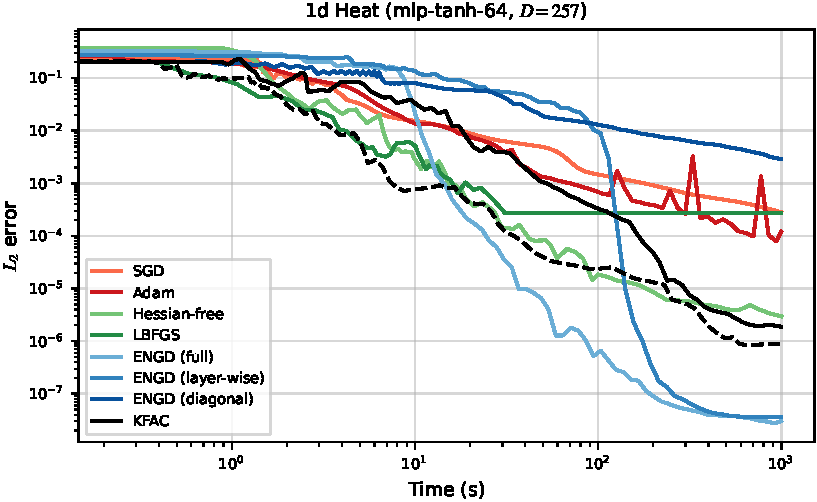
\includegraphics[trim={0 1.3cm 0 0},clip]{\pathToFigs/l2_error_over_time.pdf}
    % trim the legend and titles
    % [trim={left bottom right top},clip]
    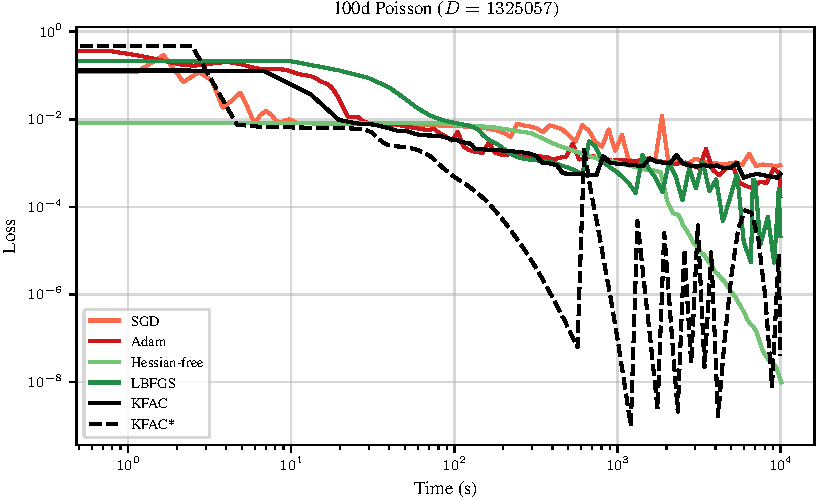
\includegraphics[trim={0 0.8cm 0 0.3cm},clip]{\pathToFigs/loss_over_time.pdf}
  \end{subfigure}
  \begin{subfigure}[t]{1.0\linewidth}
    \caption{}\label{subfig:poisson5d-step}
    % trim the legend, xlabel and xticklabels
    % [trim={left bottom right top},clip]
    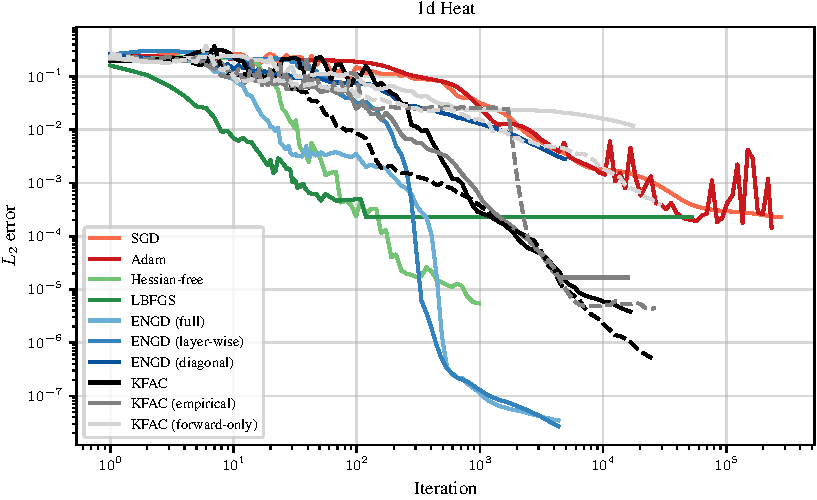
\includegraphics[trim={0 1.3cm 0 0.3cm},clip]{\pathToFigs/l2_error_over_step.pdf}
    % trim the titles
    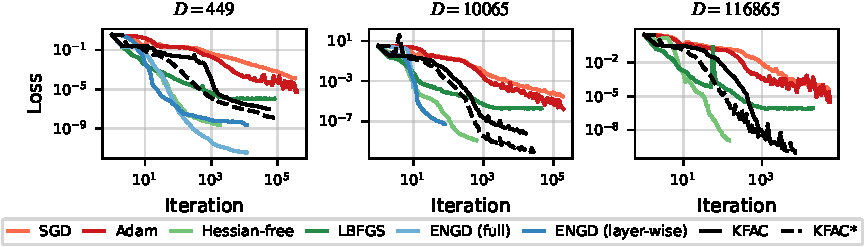
\includegraphics[trim={0 0 0 0.3cm},clip]{\pathToFigs/loss_over_step.pdf}
  \end{subfigure}
  \caption{Training loss and evaluation $L_2$ error for learning the solution to a 5d Poisson equation over (\subref{subfig:poisson5d-time}) time and (\subref{subfig:poisson5d-step}) steps.
    Columns are different neural networks.}\label{fig:poisson5d-appendix}
\end{figure}

\paragraph{Best run details}
The runs shown in \Cref{fig:poisson5d-appendix} correspond to the following hyper-parameters:
\begin{itemize}
\item $5\to 64\to 1$ MLP with $D=449$
  \begin{itemize}
    \def\pathToRuns{kfac_pinns_exp/exp10_reproduce_poisson5d/tex}
  \item \textbf{SGD:} learning rate: $\num[scientific-notation=true]{1.007555e-03}$, momentum: $\num[scientific-notation=true]{0.9}$
  \item \textbf{Adam:} learning rate: $\num[scientific-notation=true]{1.369294e-06}$, $N_{\Omega}$: $\num[scientific-notation=false]{203}$, $N_{\partial\Omega}$: $\num[scientific-notation=false]{1494}$, batch sampling frequency: $\num[scientific-notation=false]{9712}$
  \item \textbf{Hessian-free:} curvature matrix: $\text{GGN}$, initial damping: $\num[scientific-notation=true]{1.146081e-02}$, constant damping: $\text{no}$, maximum CG iterations: $\num[scientific-notation=false]{484}$, $N_{\Omega}$: $\num[scientific-notation=false]{2410}$, $N_{\partial\Omega}$: $\num[scientific-notation=false]{2448}$, batch sampling frequency: $\num[scientific-notation=false]{1311}$
  \item \textbf{LBFGS:} learning rate: $\num[scientific-notation=true]{0.2}$, history size: $\num[scientific-notation=false]{225}$
  \item \textbf{ENGD (full):} damping: $\num[scientific-notation=true]{1e-10}$, exponential moving average: $\num[scientific-notation=true]{0.3}$, initialize Gramian to identity: $\text{yes}$
  \item \textbf{ENGD (layer-wise):} damping: $\num[scientific-notation=true]{1e-06}$, exponential moving average: $\num[scientific-notation=true]{0.3}$, initialize Gramian to identity: $\text{no}$
  \item \textbf{KFAC:} damping: $\num[scientific-notation=true]{8.435180e-14}$, momentum: $\num[scientific-notation=true]{9.718645e-01}$, exponential moving average: $\num[scientific-notation=true]{9.800744e-01}$, initialize Kronecker factors to identity: $\text{yes}$, $N_{\Omega}$: $\num[scientific-notation=false]{2525}$, $N_{\partial\Omega}$: $\num[scientific-notation=false]{2663}$, batch sampling frequency: $\num[scientific-notation=false]{7916}$
  \item \textbf{KFAC*:} damping: $\num[scientific-notation=true]{2.965060e-08}$, exponential moving average: $\num[scientific-notation=true]{9.574717e-01}$, initialize Kronecker factors to identity: $\text{yes}$
  \end{itemize}

\item $5 \to 64 \to 64 \to 48 \to 48 \to 1$ MLP with $D=\num{10065}$
  \begin{itemize}
    \def\pathToRuns{kfac_pinns_exp/exp16_poisson5d_deepwide/tex}
  \item \textbf{SGD:} learning rate: $\num[scientific-notation=true]{1.007555e-03}$, momentum: $\num[scientific-notation=true]{0.9}$
  \item \textbf{Adam:} learning rate: $\num[scientific-notation=true]{1.369294e-06}$, $N_{\Omega}$: $\num[scientific-notation=false]{203}$, $N_{\partial\Omega}$: $\num[scientific-notation=false]{1494}$, batch sampling frequency: $\num[scientific-notation=false]{9712}$
  \item \textbf{Hessian-free:} curvature matrix: $\text{GGN}$, initial damping: $\num[scientific-notation=true]{1.146081e-02}$, constant damping: $\text{no}$, maximum CG iterations: $\num[scientific-notation=false]{484}$, $N_{\Omega}$: $\num[scientific-notation=false]{2410}$, $N_{\partial\Omega}$: $\num[scientific-notation=false]{2448}$, batch sampling frequency: $\num[scientific-notation=false]{1311}$
  \item \textbf{LBFGS:} learning rate: $\num[scientific-notation=true]{0.2}$, history size: $\num[scientific-notation=false]{225}$
  \item \textbf{ENGD (full):} damping: $\num[scientific-notation=true]{1e-10}$, exponential moving average: $\num[scientific-notation=true]{0.3}$, initialize Gramian to identity: $\text{yes}$
  \item \textbf{ENGD (layer-wise):} damping: $\num[scientific-notation=true]{1e-06}$, exponential moving average: $\num[scientific-notation=true]{0.3}$, initialize Gramian to identity: $\text{no}$
  \item \textbf{KFAC:} damping: $\num[scientific-notation=true]{8.435180e-14}$, momentum: $\num[scientific-notation=true]{9.718645e-01}$, exponential moving average: $\num[scientific-notation=true]{9.800744e-01}$, initialize Kronecker factors to identity: $\text{yes}$, $N_{\Omega}$: $\num[scientific-notation=false]{2525}$, $N_{\partial\Omega}$: $\num[scientific-notation=false]{2663}$, batch sampling frequency: $\num[scientific-notation=false]{7916}$
  \item \textbf{KFAC*:} damping: $\num[scientific-notation=true]{2.965060e-08}$, exponential moving average: $\num[scientific-notation=true]{9.574717e-01}$, initialize Kronecker factors to identity: $\text{yes}$
  \end{itemize}

\item $5 \to 256 \to 256\to 128 \to 128 \to 1$ MLP with $D=\num{116865}$
  \begin{itemize}
    \def\pathToRuns{kfac_pinns_exp/exp19_poisson5d_mlp_tanh_256/tex}
  \item \textbf{SGD:} learning rate: $\num[scientific-notation=true]{1.007555e-03}$, momentum: $\num[scientific-notation=true]{0.9}$
  \item \textbf{Adam:} learning rate: $\num[scientific-notation=true]{1.369294e-06}$, $N_{\Omega}$: $\num[scientific-notation=false]{203}$, $N_{\partial\Omega}$: $\num[scientific-notation=false]{1494}$, batch sampling frequency: $\num[scientific-notation=false]{9712}$
  \item \textbf{Hessian-free:} curvature matrix: $\text{GGN}$, initial damping: $\num[scientific-notation=true]{1.146081e-02}$, constant damping: $\text{no}$, maximum CG iterations: $\num[scientific-notation=false]{484}$, $N_{\Omega}$: $\num[scientific-notation=false]{2410}$, $N_{\partial\Omega}$: $\num[scientific-notation=false]{2448}$, batch sampling frequency: $\num[scientific-notation=false]{1311}$
  \item \textbf{LBFGS:} learning rate: $\num[scientific-notation=true]{0.2}$, history size: $\num[scientific-notation=false]{225}$
  \item \textbf{KFAC:} damping: $\num[scientific-notation=true]{8.435180e-14}$, momentum: $\num[scientific-notation=true]{9.718645e-01}$, exponential moving average: $\num[scientific-notation=true]{9.800744e-01}$, initialize Kronecker factors to identity: $\text{yes}$, $N_{\Omega}$: $\num[scientific-notation=false]{2525}$, $N_{\partial\Omega}$: $\num[scientific-notation=false]{2663}$, batch sampling frequency: $\num[scientific-notation=false]{7916}$
  \item \textbf{KFAC*:} damping: $\num[scientific-notation=true]{2.965060e-08}$, exponential moving average: $\num[scientific-notation=true]{9.574717e-01}$, initialize Kronecker factors to identity: $\text{yes}$
  \end{itemize}
\end{itemize}

\paragraph{Search space details} The runs shown in \Cref{fig:poisson5d-appendix} were determined to be the best via a search with approximately 50 runs on the following search spaces which were obtained by refining an initially wider search ($\mathcal{U}$ denotes a uniform, and $\mathcal{LU}$ a log-uniform distribution):
\begin{itemize}
\item $5\to 64\to 1$ MLP with $D=449$
  \begin{itemize}
    \def\pathToRuns{kfac_pinns_exp/exp10_reproduce_poisson5d/tex}
  \item \textbf{SGD:} learning rate: $\mathcal{LU}([\num[scientific-notation=true]{1e-06}; \num[scientific-notation=false]{1}])$, momentum: $\mathcal{U}([\num[scientific-notation=false]{0}; \num[scientific-notation=true]{0.99}])$, $N_{\Omega}$: $\mathcal{C}(\{\num[scientific-notation=false]{100},\num[scientific-notation=false]{101},\text{\dots},\num[scientific-notation=false]{5000}\})$, $N_{\partial\Omega}$: $\mathcal{C}(\{\num[scientific-notation=false]{50},\num[scientific-notation=false]{51},\text{\dots},\num[scientific-notation=false]{2500}\})$, batch sampling frequency: $\mathcal{C}(\{\num[scientific-notation=false]{0},\num[scientific-notation=false]{1},\text{\dots},\num[scientific-notation=false]{1000}\})$
  \item \textbf{Adam:} learning rate: $\mathcal{LU}([\num[scientific-notation=true]{0.0001}; \num[scientific-notation=true]{0.5}])$
  \item \textbf{Hessian-free:} curvature matrix: $\mathcal{U}(\{\text{GGN},\text{Hessian}\})$, initial damping: $\mathcal{LU}([\num[scientific-notation=true]{1e-15}; \num[scientific-notation=false]{1}])$, constant damping: $\mathcal{U}(\{\text{no},\text{yes}\})$, maximum CG iterations: $\mathcal{U}(\{\num[scientific-notation=false]{1},\num[scientific-notation=false]{2},\text{\dots},\num[scientific-notation=false]{500}\})$, $N_{\Omega}$: $\mathcal{U}(\{\num[scientific-notation=false]{100},\num[scientific-notation=false]{101},\text{\dots},\num[scientific-notation=false]{5000}\})$, $N_{\partial\Omega}$: $\mathcal{U}(\{\num[scientific-notation=false]{50},\num[scientific-notation=false]{51},\text{\dots},\num[scientific-notation=false]{2500}\})$, batch sampling frequency: $\mathcal{U}(\{\num[scientific-notation=false]{0},\num[scientific-notation=false]{1},\text{\dots},\num[scientific-notation=false]{5000}\})$
  \item \textbf{LBFGS:} learning rate: $\mathcal{C}(\{\num[scientific-notation=true]{0.5},\num[scientific-notation=true]{0.2},\num[scientific-notation=true]{0.1},\num[scientific-notation=true]{0.05},\num[scientific-notation=true]{0.02},\num[scientific-notation=true]{0.01}\})$, history size: $\mathcal{C}(\{\num[scientific-notation=false]{75},\num[scientific-notation=false]{100},\num[scientific-notation=false]{125},\num[scientific-notation=false]{150},\num[scientific-notation=false]{175},\num[scientific-notation=false]{200},\num[scientific-notation=false]{225},\num[scientific-notation=false]{250}\})$
  \item \textbf{ENGD (full):} damping: $\mathcal{C}(\{\num[scientific-notation=true]{1e-08},\num[scientific-notation=true]{1e-09},\num[scientific-notation=true]{1e-10},\num[scientific-notation=true]{1e-11},\num[scientific-notation=true]{1e-12},\num[scientific-notation=false]{0}\})$, exponential moving average: $\mathcal{C}(\{\num[scientific-notation=false]{0},\num[scientific-notation=true]{0.3},\num[scientific-notation=true]{0.6},\num[scientific-notation=true]{0.9}\})$, initialize Gramian to identity: $\mathcal{C}(\{\text{no},\text{yes}\})$
  \item \textbf{ENGD (layer-wise):} damping: $\mathcal{U}(\{\num[scientific-notation=true]{0.01},\num[scientific-notation=true]{0.001},\num[scientific-notation=true]{0.0001},\num[scientific-notation=true]{1e-05},\num[scientific-notation=true]{1e-06}\})$, exponential moving average: $\mathcal{U}(\{\num[scientific-notation=false]{0},\num[scientific-notation=true]{0.3},\num[scientific-notation=true]{0.6},\num[scientific-notation=true]{0.9},\num[scientific-notation=true]{0.99}\})$, initialize Gramian to identity: $\mathcal{U}(\{\text{no},\text{yes}\})$
  \item \textbf{KFAC:} damping: $\mathcal{LU}([\num[scientific-notation=true]{1e-15}; \num[scientific-notation=true]{0.01}])$, momentum: $\mathcal{U}([\num[scientific-notation=false]{0}; \num[scientific-notation=true]{0.99}])$, exponential moving average: $\mathcal{U}([\num[scientific-notation=false]{0}; \num[scientific-notation=true]{0.99}])$, initialize Kronecker factors to identity: $\mathcal{C}(\{\text{no},\text{yes}\})$
  \item \textbf{KFAC*:} damping: $\mathcal{LU}([\num[scientific-notation=true]{1e-15}; \num[scientific-notation=true]{0.01}])$, exponential moving average: $\mathcal{U}([\num[scientific-notation=false]{0}; \num[scientific-notation=true]{0.99}])$, initialize Kronecker factors to identity: $\mathcal{U}(\{\text{no},\text{yes}\})$, $N_{\Omega}$: $\mathcal{U}(\{\num[scientific-notation=false]{100},\num[scientific-notation=false]{101},\text{\dots},\num[scientific-notation=false]{5000}\})$, $N_{\partial\Omega}$: $\mathcal{U}(\{\num[scientific-notation=false]{50},\num[scientific-notation=false]{51},\text{\dots},\num[scientific-notation=false]{2500}\})$, batch sampling frequency: $\mathcal{U}(\{\num[scientific-notation=false]{0},\num[scientific-notation=false]{1},\text{\dots},\num[scientific-notation=false]{5000}\})$
  \end{itemize}

\item $5 \to 64 \to 64 \to 48 \to 48 \to 1$ MLP with $D=\num{10065}$
  \begin{itemize}
    \def\pathToRuns{kfac_pinns_exp/exp16_poisson5d_deepwide/tex}
  \item \textbf{SGD:} learning rate: $\mathcal{LU}([\num[scientific-notation=true]{1e-06}; \num[scientific-notation=false]{1}])$, momentum: $\mathcal{U}([\num[scientific-notation=false]{0}; \num[scientific-notation=true]{0.99}])$, $N_{\Omega}$: $\mathcal{C}(\{\num[scientific-notation=false]{100},\num[scientific-notation=false]{101},\text{\dots},\num[scientific-notation=false]{5000}\})$, $N_{\partial\Omega}$: $\mathcal{C}(\{\num[scientific-notation=false]{50},\num[scientific-notation=false]{51},\text{\dots},\num[scientific-notation=false]{2500}\})$, batch sampling frequency: $\mathcal{C}(\{\num[scientific-notation=false]{0},\num[scientific-notation=false]{1},\text{\dots},\num[scientific-notation=false]{1000}\})$
  \item \textbf{Adam:} learning rate: $\mathcal{LU}([\num[scientific-notation=true]{0.0001}; \num[scientific-notation=true]{0.5}])$
  \item \textbf{Hessian-free:} curvature matrix: $\mathcal{U}(\{\text{GGN},\text{Hessian}\})$, initial damping: $\mathcal{LU}([\num[scientific-notation=true]{1e-15}; \num[scientific-notation=false]{1}])$, constant damping: $\mathcal{U}(\{\text{no},\text{yes}\})$, maximum CG iterations: $\mathcal{U}(\{\num[scientific-notation=false]{1},\num[scientific-notation=false]{2},\text{\dots},\num[scientific-notation=false]{500}\})$, $N_{\Omega}$: $\mathcal{U}(\{\num[scientific-notation=false]{100},\num[scientific-notation=false]{101},\text{\dots},\num[scientific-notation=false]{5000}\})$, $N_{\partial\Omega}$: $\mathcal{U}(\{\num[scientific-notation=false]{50},\num[scientific-notation=false]{51},\text{\dots},\num[scientific-notation=false]{2500}\})$, batch sampling frequency: $\mathcal{U}(\{\num[scientific-notation=false]{0},\num[scientific-notation=false]{1},\text{\dots},\num[scientific-notation=false]{5000}\})$
  \item \textbf{LBFGS:} learning rate: $\mathcal{C}(\{\num[scientific-notation=true]{0.5},\num[scientific-notation=true]{0.2},\num[scientific-notation=true]{0.1},\num[scientific-notation=true]{0.05},\num[scientific-notation=true]{0.02},\num[scientific-notation=true]{0.01}\})$, history size: $\mathcal{C}(\{\num[scientific-notation=false]{75},\num[scientific-notation=false]{100},\num[scientific-notation=false]{125},\num[scientific-notation=false]{150},\num[scientific-notation=false]{175},\num[scientific-notation=false]{200},\num[scientific-notation=false]{225},\num[scientific-notation=false]{250}\})$
  \item \textbf{ENGD (full):} damping: $\mathcal{C}(\{\num[scientific-notation=true]{1e-08},\num[scientific-notation=true]{1e-09},\num[scientific-notation=true]{1e-10},\num[scientific-notation=true]{1e-11},\num[scientific-notation=true]{1e-12},\num[scientific-notation=false]{0}\})$, exponential moving average: $\mathcal{C}(\{\num[scientific-notation=false]{0},\num[scientific-notation=true]{0.3},\num[scientific-notation=true]{0.6},\num[scientific-notation=true]{0.9}\})$, initialize Gramian to identity: $\mathcal{C}(\{\text{no},\text{yes}\})$
  \item \textbf{ENGD (layer-wise):} damping: $\mathcal{U}(\{\num[scientific-notation=true]{0.01},\num[scientific-notation=true]{0.001},\num[scientific-notation=true]{0.0001},\num[scientific-notation=true]{1e-05},\num[scientific-notation=true]{1e-06}\})$, exponential moving average: $\mathcal{U}(\{\num[scientific-notation=false]{0},\num[scientific-notation=true]{0.3},\num[scientific-notation=true]{0.6},\num[scientific-notation=true]{0.9},\num[scientific-notation=true]{0.99}\})$, initialize Gramian to identity: $\mathcal{U}(\{\text{no},\text{yes}\})$
  \item \textbf{KFAC:} damping: $\mathcal{LU}([\num[scientific-notation=true]{1e-15}; \num[scientific-notation=true]{0.01}])$, momentum: $\mathcal{U}([\num[scientific-notation=false]{0}; \num[scientific-notation=true]{0.99}])$, exponential moving average: $\mathcal{U}([\num[scientific-notation=false]{0}; \num[scientific-notation=true]{0.99}])$, initialize Kronecker factors to identity: $\mathcal{C}(\{\text{no},\text{yes}\})$
  \item \textbf{KFAC*:} damping: $\mathcal{LU}([\num[scientific-notation=true]{1e-15}; \num[scientific-notation=true]{0.01}])$, exponential moving average: $\mathcal{U}([\num[scientific-notation=false]{0}; \num[scientific-notation=true]{0.99}])$, initialize Kronecker factors to identity: $\mathcal{U}(\{\text{no},\text{yes}\})$, $N_{\Omega}$: $\mathcal{U}(\{\num[scientific-notation=false]{100},\num[scientific-notation=false]{101},\text{\dots},\num[scientific-notation=false]{5000}\})$, $N_{\partial\Omega}$: $\mathcal{U}(\{\num[scientific-notation=false]{50},\num[scientific-notation=false]{51},\text{\dots},\num[scientific-notation=false]{2500}\})$, batch sampling frequency: $\mathcal{U}(\{\num[scientific-notation=false]{0},\num[scientific-notation=false]{1},\text{\dots},\num[scientific-notation=false]{5000}\})$
  \end{itemize}

\item $5 \to 256 \to 256\to 128 \to 128 \to 1$ MLP with $D=\num{116865}$
  \begin{itemize}
    \def\pathToRuns{kfac_pinns_exp/exp19_poisson5d_mlp_tanh_256/tex}
  \item \textbf{SGD:} learning rate: $\mathcal{LU}([\num[scientific-notation=true]{1e-06}; \num[scientific-notation=false]{1}])$, momentum: $\mathcal{U}([\num[scientific-notation=false]{0}; \num[scientific-notation=true]{0.99}])$, $N_{\Omega}$: $\mathcal{C}(\{\num[scientific-notation=false]{100},\num[scientific-notation=false]{101},\text{\dots},\num[scientific-notation=false]{5000}\})$, $N_{\partial\Omega}$: $\mathcal{C}(\{\num[scientific-notation=false]{50},\num[scientific-notation=false]{51},\text{\dots},\num[scientific-notation=false]{2500}\})$, batch sampling frequency: $\mathcal{C}(\{\num[scientific-notation=false]{0},\num[scientific-notation=false]{1},\text{\dots},\num[scientific-notation=false]{1000}\})$
  \item \textbf{Adam:} learning rate: $\mathcal{LU}([\num[scientific-notation=true]{0.0001}; \num[scientific-notation=true]{0.5}])$
  \item \textbf{Hessian-free:} curvature matrix: $\mathcal{U}(\{\text{GGN},\text{Hessian}\})$, initial damping: $\mathcal{LU}([\num[scientific-notation=true]{1e-15}; \num[scientific-notation=false]{1}])$, constant damping: $\mathcal{U}(\{\text{no},\text{yes}\})$, maximum CG iterations: $\mathcal{U}(\{\num[scientific-notation=false]{1},\num[scientific-notation=false]{2},\text{\dots},\num[scientific-notation=false]{500}\})$, $N_{\Omega}$: $\mathcal{U}(\{\num[scientific-notation=false]{100},\num[scientific-notation=false]{101},\text{\dots},\num[scientific-notation=false]{5000}\})$, $N_{\partial\Omega}$: $\mathcal{U}(\{\num[scientific-notation=false]{50},\num[scientific-notation=false]{51},\text{\dots},\num[scientific-notation=false]{2500}\})$, batch sampling frequency: $\mathcal{U}(\{\num[scientific-notation=false]{0},\num[scientific-notation=false]{1},\text{\dots},\num[scientific-notation=false]{5000}\})$
  \item \textbf{LBFGS:} learning rate: $\mathcal{C}(\{\num[scientific-notation=true]{0.5},\num[scientific-notation=true]{0.2},\num[scientific-notation=true]{0.1},\num[scientific-notation=true]{0.05},\num[scientific-notation=true]{0.02},\num[scientific-notation=true]{0.01}\})$, history size: $\mathcal{C}(\{\num[scientific-notation=false]{75},\num[scientific-notation=false]{100},\num[scientific-notation=false]{125},\num[scientific-notation=false]{150},\num[scientific-notation=false]{175},\num[scientific-notation=false]{200},\num[scientific-notation=false]{225},\num[scientific-notation=false]{250}\})$
  \item \textbf{KFAC:} damping: $\mathcal{LU}([\num[scientific-notation=true]{1e-15}; \num[scientific-notation=true]{0.01}])$, momentum: $\mathcal{U}([\num[scientific-notation=false]{0}; \num[scientific-notation=true]{0.99}])$, exponential moving average: $\mathcal{U}([\num[scientific-notation=false]{0}; \num[scientific-notation=true]{0.99}])$, initialize Kronecker factors to identity: $\mathcal{C}(\{\text{no},\text{yes}\})$
  \item \textbf{KFAC*:} damping: $\mathcal{LU}([\num[scientific-notation=true]{1e-15}; \num[scientific-notation=true]{0.01}])$, exponential moving average: $\mathcal{U}([\num[scientific-notation=false]{0}; \num[scientific-notation=true]{0.99}])$, initialize Kronecker factors to identity: $\mathcal{U}(\{\text{no},\text{yes}\})$, $N_{\Omega}$: $\mathcal{U}(\{\num[scientific-notation=false]{100},\num[scientific-notation=false]{101},\text{\dots},\num[scientific-notation=false]{5000}\})$, $N_{\partial\Omega}$: $\mathcal{U}(\{\num[scientific-notation=false]{50},\num[scientific-notation=false]{51},\text{\dots},\num[scientific-notation=false]{2500}\})$, batch sampling frequency: $\mathcal{U}(\{\num[scientific-notation=false]{0},\num[scientific-notation=false]{1},\text{\dots},\num[scientific-notation=false]{5000}\})$
  \end{itemize}
\end{itemize}

\subsection{10d Poisson Equation}\label{sec:poisson10d-appendix}

\paragraph{Setup} We consider a 10-dimensional Poisson equation $-\Delta u(\vx) = 0$ on the 10-dimensional unit square $\vx \in [0, 1]^5$ with zero right-hand side and harmonic mixed second order polynomial boundary conditions $u(\vx) = \sum_{i=1}^{\nicefrac{d}{2}} \evx_{2i-1} \evx_{2i}$ for $\vx \in \partial [0,1]^d$.
We sample training batches of size $N_{\Omega} = \num{3000}, N_{\partial\Omega} = 1000$ and evaluate the $L_2$ error on a separate set of $\num{30000}$ data points using the known solution $u_{\star}(\vx) = \sum_{i=1}^{\nicefrac{d}{2}} \evx_{2i-1} \evx_{2i}$.
All optimizers except for KFAC sample a new training batch each iteration.
KFAC only re-samples every 100 iterations because we noticed significant improvement with multiple iterations on a fixed batch.
Each run is limited to $\num{6000}\,\text{s}$.
We use a $10 \to 256 \to 256\to 128 \to 128 \to 1$ MLP with $D=\num{118145}$ MLP whose linear layers are Tanh-activated except for the final one.
\Cref{fig:poisson_10d-appendix} visualizes the results.

\begin{figure}[!h]
  \centering
  \def\pathToFigs{kfac_pinns_exp/exp21_poisson_10d}
  \begin{subfigure}[t]{1.0\linewidth}
    \caption{}\label{subfig:poisson_10d-time}
    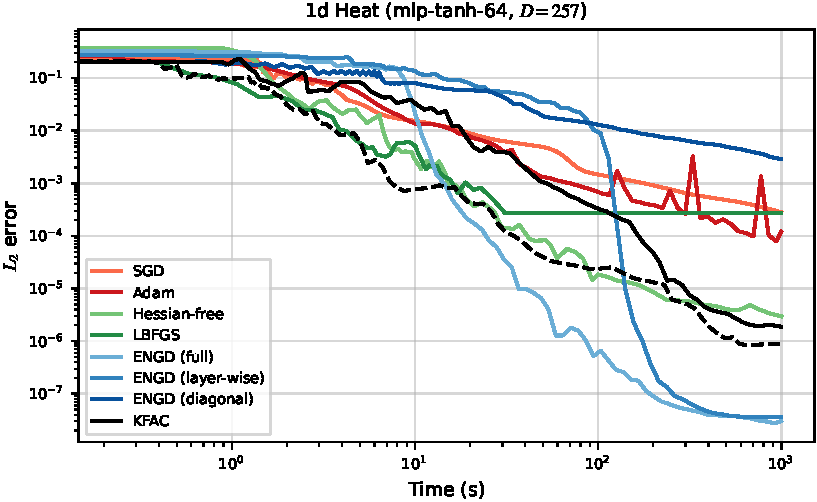
\includegraphics{\pathToFigs/l2_error_over_time.pdf}
    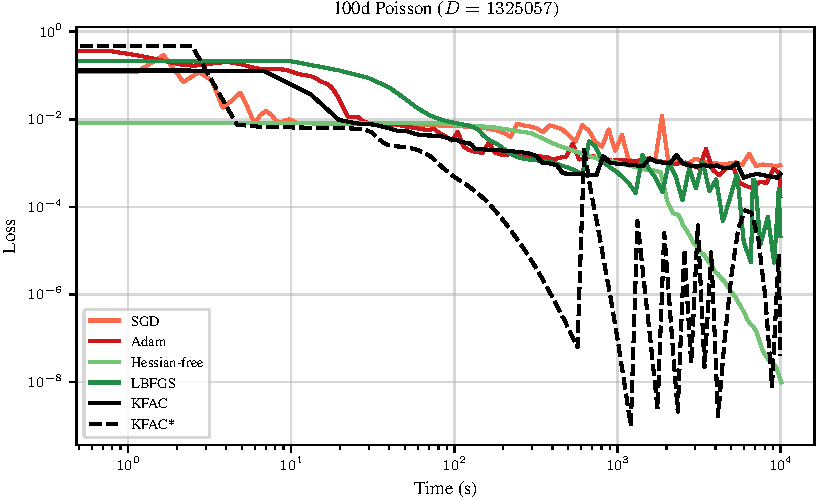
\includegraphics{\pathToFigs/loss_over_time.pdf}
  \end{subfigure}
  \begin{subfigure}[t]{1.0\linewidth}
    \caption{}\label{subfig:poisson_10d-step}
    \includegraphics{\pathToFigs/l2_error_over_step.pdf}
    \includegraphics{\pathToFigs/loss_over_step.pdf}
  \end{subfigure}
  \caption{Training loss and evaluation $L_2$ error for learning the solution to a 10d Poisson equation over (\subref{subfig:poisson_10d-time}) time and (\subref{subfig:poisson_10d-step}) steps.}\label{fig:poisson_10d-appendix}
\end{figure}

\paragraph{Best run details}
The runs shown in \Cref{fig:poisson_10d-appendix} correspond to the following hyper-parameters:
\begin{itemize}
  \def\pathToRuns{kfac_pinns_exp/exp21_poisson_10d/tex/}
\item \textbf{SGD:} learning rate: $\num[scientific-notation=true]{1.007555e-03}$, momentum: $\num[scientific-notation=true]{0.9}$
\item \textbf{Adam:} learning rate: $\num[scientific-notation=true]{1.369294e-06}$, $N_{\Omega}$: $\num[scientific-notation=false]{203}$, $N_{\partial\Omega}$: $\num[scientific-notation=false]{1494}$, batch sampling frequency: $\num[scientific-notation=false]{9712}$
\item \textbf{Hessian-free:} curvature matrix: $\text{GGN}$, initial damping: $\num[scientific-notation=true]{1.146081e-02}$, constant damping: $\text{no}$, maximum CG iterations: $\num[scientific-notation=false]{484}$, $N_{\Omega}$: $\num[scientific-notation=false]{2410}$, $N_{\partial\Omega}$: $\num[scientific-notation=false]{2448}$, batch sampling frequency: $\num[scientific-notation=false]{1311}$
\item \textbf{LBFGS:} learning rate: $\num[scientific-notation=true]{0.2}$, history size: $\num[scientific-notation=false]{225}$
\item \textbf{KFAC:} damping: $\num[scientific-notation=true]{8.435180e-14}$, momentum: $\num[scientific-notation=true]{9.718645e-01}$, exponential moving average: $\num[scientific-notation=true]{9.800744e-01}$, initialize Kronecker factors to identity: $\text{yes}$, $N_{\Omega}$: $\num[scientific-notation=false]{2525}$, $N_{\partial\Omega}$: $\num[scientific-notation=false]{2663}$, batch sampling frequency: $\num[scientific-notation=false]{7916}$
\item \textbf{KFAC*:} damping: $\num[scientific-notation=true]{2.965060e-08}$, exponential moving average: $\num[scientific-notation=true]{9.574717e-01}$, initialize Kronecker factors to identity: $\text{yes}$
\end{itemize}

\paragraph{Search space details} The runs shown in \Cref{fig:poisson_10d-appendix} were determined to be the best via a Bayesian search on the following search spaces which each optimizer given approximately the same total computational time ($\mathcal{U}$ denotes a uniform, and $\mathcal{LU}$ a log-uniform distribution):
\begin{itemize}
  \def\pathToRuns{kfac_pinns_exp/exp21_poisson_10d/tex/}
\item \textbf{SGD:} learning rate: $\mathcal{LU}([\num[scientific-notation=true]{1e-06}; \num[scientific-notation=false]{1}])$, momentum: $\mathcal{U}([\num[scientific-notation=false]{0}; \num[scientific-notation=true]{0.99}])$, $N_{\Omega}$: $\mathcal{C}(\{\num[scientific-notation=false]{100},\num[scientific-notation=false]{101},\text{\dots},\num[scientific-notation=false]{5000}\})$, $N_{\partial\Omega}$: $\mathcal{C}(\{\num[scientific-notation=false]{50},\num[scientific-notation=false]{51},\text{\dots},\num[scientific-notation=false]{2500}\})$, batch sampling frequency: $\mathcal{C}(\{\num[scientific-notation=false]{0},\num[scientific-notation=false]{1},\text{\dots},\num[scientific-notation=false]{1000}\})$
\item \textbf{Adam:} learning rate: $\mathcal{LU}([\num[scientific-notation=true]{0.0001}; \num[scientific-notation=true]{0.5}])$
\item \textbf{Hessian-free:} curvature matrix: $\mathcal{U}(\{\text{GGN},\text{Hessian}\})$, initial damping: $\mathcal{LU}([\num[scientific-notation=true]{1e-15}; \num[scientific-notation=false]{1}])$, constant damping: $\mathcal{U}(\{\text{no},\text{yes}\})$, maximum CG iterations: $\mathcal{U}(\{\num[scientific-notation=false]{1},\num[scientific-notation=false]{2},\text{\dots},\num[scientific-notation=false]{500}\})$, $N_{\Omega}$: $\mathcal{U}(\{\num[scientific-notation=false]{100},\num[scientific-notation=false]{101},\text{\dots},\num[scientific-notation=false]{5000}\})$, $N_{\partial\Omega}$: $\mathcal{U}(\{\num[scientific-notation=false]{50},\num[scientific-notation=false]{51},\text{\dots},\num[scientific-notation=false]{2500}\})$, batch sampling frequency: $\mathcal{U}(\{\num[scientific-notation=false]{0},\num[scientific-notation=false]{1},\text{\dots},\num[scientific-notation=false]{5000}\})$
\item \textbf{LBFGS:} learning rate: $\mathcal{C}(\{\num[scientific-notation=true]{0.5},\num[scientific-notation=true]{0.2},\num[scientific-notation=true]{0.1},\num[scientific-notation=true]{0.05},\num[scientific-notation=true]{0.02},\num[scientific-notation=true]{0.01}\})$, history size: $\mathcal{C}(\{\num[scientific-notation=false]{75},\num[scientific-notation=false]{100},\num[scientific-notation=false]{125},\num[scientific-notation=false]{150},\num[scientific-notation=false]{175},\num[scientific-notation=false]{200},\num[scientific-notation=false]{225},\num[scientific-notation=false]{250}\})$
\item \textbf{KFAC:} damping: $\mathcal{LU}([\num[scientific-notation=true]{1e-15}; \num[scientific-notation=true]{0.01}])$, momentum: $\mathcal{U}([\num[scientific-notation=false]{0}; \num[scientific-notation=true]{0.99}])$, exponential moving average: $\mathcal{U}([\num[scientific-notation=false]{0}; \num[scientific-notation=true]{0.99}])$, initialize Kronecker factors to identity: $\mathcal{C}(\{\text{no},\text{yes}\})$
\item \textbf{KFAC*:} damping: $\mathcal{LU}([\num[scientific-notation=true]{1e-15}; \num[scientific-notation=true]{0.01}])$, exponential moving average: $\mathcal{U}([\num[scientific-notation=false]{0}; \num[scientific-notation=true]{0.99}])$, initialize Kronecker factors to identity: $\mathcal{U}(\{\text{no},\text{yes}\})$, $N_{\Omega}$: $\mathcal{U}(\{\num[scientific-notation=false]{100},\num[scientific-notation=false]{101},\text{\dots},\num[scientific-notation=false]{5000}\})$, $N_{\partial\Omega}$: $\mathcal{U}(\{\num[scientific-notation=false]{50},\num[scientific-notation=false]{51},\text{\dots},\num[scientific-notation=false]{2500}\})$, batch sampling frequency: $\mathcal{U}(\{\num[scientific-notation=false]{0},\num[scientific-notation=false]{1},\text{\dots},\num[scientific-notation=false]{5000}\})$
\end{itemize}

\subsection{5/10/100-d Poisson Equations with Bayesian Search}\label{sec:high-dimensional-poissons-app}

\paragraph{Setup} Here, we consider three Poisson equations $- \Delta u(\vx) = f(\vx)$ with different right-hand sides and boundary conditions on the unit square $\vx \in [0, 1]^d$:
\begin{itemize}
\item $d=5$ with cosine sum right-hand side $f(\vx) = \pi^2 \sum_{i=1}^d \cos(\pi \evx_i)$, boundary conditions $u(\vx) = \sum_{i=1}^d \cos(\pi \evx_i)$ for $\vx \in \partial [0,1]^d$, and known solution $u_{\star}(\vx) = \sum_{i=1}^d \cos(\pi \evx_i)$.
  We assign each run a budget of $\num{3000}\,\text{s}$.

\item $d=10$ with zero right-hand side $f(\vx) = 0$, harmonic mixed second order polynomial boundary conditions $u(\vx) = \sum_{i=1}^{\nicefrac{d}{2}} \evx_{2i-1} \evx_{2i}$ for $\vx \in \partial [0,1]^d$, and known solution $u_{\star}(\vx) =  \sum_{i=1}^{\nicefrac{d}{2}} \evx_{2i-1} \evx_{2i}$.
  We assign each run a budget of $\num{6000}\,\text{s}$.

\item $d=100$ with constant non-zero right-hand side $f(\vx) = -2 d$, square norm boundary conditions $u(\vx) = \left\lVert \vx \right\rVert_2^2$ for $\vx \in \partial [0,1]^d$, and known solution $u_{\star}(\vx) =  \left\lVert \vx \right\rVert_2^2$.
  We assign each run a budget of $\num{10000}\,\text{s}$.
\end{itemize}
We tune the optimizer-hyperparameters described in \Cref{sec:tuning-protocol}, as well as the batch sizes $N_{\Omega}, N_{\partial \Omega}$, and their associated re-sampling frequencies using Bayesian search.
We use five layer MLP architectures with varying widths whose layers are Tanh-activated except for the final layer.
These architectures are too large to be optimized by ENGD.
\Cref{fig:poisson-bayes-appendix} visualizes the results.

\begin{figure}[!h]
  \centering
  \def\pathToFigs{kfac_pinns_exp/exp33_poisson_bayes_groupplot}
  \begin{subfigure}[t]{1.0\linewidth}
    \caption{}\label{subfig:poisson-bayes-time}
    % trim legend, xlabel and xticklabels
    % [trim={left bottom right top},clip]
    \includegraphics[trim={0 1.3cm 0 0},clip]{\pathToFigs/l2_error_over_time.pdf}
    % trim the legend and titles
    % [trim={left bottom right top},clip]
    \includegraphics[trim={0 0.5cm 0 0.3cm},clip]{\pathToFigs/loss_over_time.pdf}
  \end{subfigure}
  \begin{subfigure}[t]{1.0\linewidth}
    \caption{}\label{subfig:poisson-bayes-step}
    % trim the legend, xlabel and xticklabels
    % [trim={left bottom right top},clip]
    \includegraphics[trim={0 1.3cm 0 0.3cm},clip]{\pathToFigs/l2_error_over_step.pdf}
    % trim the titles
    \includegraphics[trim={0 0 0 0.3cm},clip]{\pathToFigs/loss_over_step.pdf}
  \end{subfigure}
  \caption{Training loss and evaluation $L_2$ error for learning the solution to high-dimensional Poisson equations over (\subref{subfig:poisson-bayes-time}) time and (\subref{subfig:poisson-bayes-step}) steps using Bayesian search.}\label{fig:poisson-bayes-appendix}
\end{figure}

\paragraph{Best run details} The runs shown in \Cref{fig:poisson-bayes-appendix} correspond to the following hyper-parameters:

\begin{itemize}

\item 5d Poisson equation, $5 \to 256 \to 256 \to 128 \to 128 \to 1$ MLP with $D=\num{116865}$
  \begin{itemize}
    \def\pathToRuns{kfac_pinns_exp/exp26_poisson5d_mlp_tanh_256_bayes/tex}
  \item \textbf{SGD:} learning rate: $\num[scientific-notation=true]{1.007555e-03}$, momentum: $\num[scientific-notation=true]{0.9}$
  \item \textbf{Adam:} learning rate: $\num[scientific-notation=true]{1.369294e-06}$, $N_{\Omega}$: $\num[scientific-notation=false]{203}$, $N_{\partial\Omega}$: $\num[scientific-notation=false]{1494}$, batch sampling frequency: $\num[scientific-notation=false]{9712}$
  \item \textbf{Hessian-free:} curvature matrix: $\text{GGN}$, initial damping: $\num[scientific-notation=true]{1.146081e-02}$, constant damping: $\text{no}$, maximum CG iterations: $\num[scientific-notation=false]{484}$, $N_{\Omega}$: $\num[scientific-notation=false]{2410}$, $N_{\partial\Omega}$: $\num[scientific-notation=false]{2448}$, batch sampling frequency: $\num[scientific-notation=false]{1311}$
  \item \textbf{LBFGS:} learning rate: $\num[scientific-notation=true]{0.2}$, history size: $\num[scientific-notation=false]{225}$
  \item \textbf{KFAC:} damping: $\num[scientific-notation=true]{8.435180e-14}$, momentum: $\num[scientific-notation=true]{9.718645e-01}$, exponential moving average: $\num[scientific-notation=true]{9.800744e-01}$, initialize Kronecker factors to identity: $\text{yes}$, $N_{\Omega}$: $\num[scientific-notation=false]{2525}$, $N_{\partial\Omega}$: $\num[scientific-notation=false]{2663}$, batch sampling frequency: $\num[scientific-notation=false]{7916}$
  \item \textbf{KFAC*:} damping: $\num[scientific-notation=true]{2.965060e-08}$, exponential moving average: $\num[scientific-notation=true]{9.574717e-01}$, initialize Kronecker factors to identity: $\text{yes}$
  \end{itemize}

\item 10d Poisson equation, $10 \to 256 \to 256 \to 128 \to 128 \to 1$ MLP with $D=\num{118145}$
  \begin{itemize}
    \def\pathToRuns{kfac_pinns_exp/exp32_poisson10d_mlp_tanh_256_bayes/tex}
  \item \textbf{SGD:} learning rate: $\num[scientific-notation=true]{1.007555e-03}$, momentum: $\num[scientific-notation=true]{0.9}$
  \item \textbf{Adam:} learning rate: $\num[scientific-notation=true]{1.369294e-06}$, $N_{\Omega}$: $\num[scientific-notation=false]{203}$, $N_{\partial\Omega}$: $\num[scientific-notation=false]{1494}$, batch sampling frequency: $\num[scientific-notation=false]{9712}$
  \item \textbf{Hessian-free:} curvature matrix: $\text{GGN}$, initial damping: $\num[scientific-notation=true]{1.146081e-02}$, constant damping: $\text{no}$, maximum CG iterations: $\num[scientific-notation=false]{484}$, $N_{\Omega}$: $\num[scientific-notation=false]{2410}$, $N_{\partial\Omega}$: $\num[scientific-notation=false]{2448}$, batch sampling frequency: $\num[scientific-notation=false]{1311}$
  \item \textbf{LBFGS:} learning rate: $\num[scientific-notation=true]{0.2}$, history size: $\num[scientific-notation=false]{225}$
  \item \textbf{KFAC:} damping: $\num[scientific-notation=true]{8.435180e-14}$, momentum: $\num[scientific-notation=true]{9.718645e-01}$, exponential moving average: $\num[scientific-notation=true]{9.800744e-01}$, initialize Kronecker factors to identity: $\text{yes}$, $N_{\Omega}$: $\num[scientific-notation=false]{2525}$, $N_{\partial\Omega}$: $\num[scientific-notation=false]{2663}$, batch sampling frequency: $\num[scientific-notation=false]{7916}$
  \item \textbf{KFAC*:} damping: $\num[scientific-notation=true]{2.965060e-08}$, exponential moving average: $\num[scientific-notation=true]{9.574717e-01}$, initialize Kronecker factors to identity: $\text{yes}$
  \end{itemize}

\item 100d Poisson equation, $100 \to 768 \to 768 \to 512 \to 512 \to 1$ MLP with $D=\num{1325057}$
  \begin{itemize}
    \def\pathToRuns{kfac_pinns_exp/exp14_poisson_100d_weinan/tex}
  \item \textbf{SGD:} learning rate: $\num[scientific-notation=true]{1.007555e-03}$, momentum: $\num[scientific-notation=true]{0.9}$
  \item \textbf{Adam:} learning rate: $\num[scientific-notation=true]{1.369294e-06}$, $N_{\Omega}$: $\num[scientific-notation=false]{203}$, $N_{\partial\Omega}$: $\num[scientific-notation=false]{1494}$, batch sampling frequency: $\num[scientific-notation=false]{9712}$
  \item \textbf{Hessian-free:} curvature matrix: $\text{GGN}$, initial damping: $\num[scientific-notation=true]{1.146081e-02}$, constant damping: $\text{no}$, maximum CG iterations: $\num[scientific-notation=false]{484}$, $N_{\Omega}$: $\num[scientific-notation=false]{2410}$, $N_{\partial\Omega}$: $\num[scientific-notation=false]{2448}$, batch sampling frequency: $\num[scientific-notation=false]{1311}$
  \item \textbf{LBFGS:} learning rate: $\num[scientific-notation=true]{0.2}$, history size: $\num[scientific-notation=false]{225}$
  \item \textbf{KFAC:} damping: $\num[scientific-notation=true]{8.435180e-14}$, momentum: $\num[scientific-notation=true]{9.718645e-01}$, exponential moving average: $\num[scientific-notation=true]{9.800744e-01}$, initialize Kronecker factors to identity: $\text{yes}$, $N_{\Omega}$: $\num[scientific-notation=false]{2525}$, $N_{\partial\Omega}$: $\num[scientific-notation=false]{2663}$, batch sampling frequency: $\num[scientific-notation=false]{7916}$
  \item \textbf{KFAC*:} damping: $\num[scientific-notation=true]{2.965060e-08}$, exponential moving average: $\num[scientific-notation=true]{9.574717e-01}$, initialize Kronecker factors to identity: $\text{yes}$
  \end{itemize}
\end{itemize}

\paragraph{Search space details} The runs shown in \Cref{fig:poisson-bayes-appendix} were determined to be the best via a Bayesian search on the following search spaces which each optimizer given approximately the same total computational time ($\mathcal{U}$ denotes a uniform, and $\mathcal{LU}$ a log-uniform distribution):
\begin{itemize}

\item 5d Poisson equation, $5 \to 256 \to 256 \to 128 \to 128 \to 1$ MLP with $D=\num{116865}$
  \begin{itemize}
    \def\pathToRuns{kfac_pinns_exp/exp26_poisson5d_mlp_tanh_256_bayes/tex}
  \item \textbf{SGD:} learning rate: $\mathcal{LU}([\num[scientific-notation=true]{1e-06}; \num[scientific-notation=false]{1}])$, momentum: $\mathcal{U}([\num[scientific-notation=false]{0}; \num[scientific-notation=true]{0.99}])$, $N_{\Omega}$: $\mathcal{C}(\{\num[scientific-notation=false]{100},\num[scientific-notation=false]{101},\text{\dots},\num[scientific-notation=false]{5000}\})$, $N_{\partial\Omega}$: $\mathcal{C}(\{\num[scientific-notation=false]{50},\num[scientific-notation=false]{51},\text{\dots},\num[scientific-notation=false]{2500}\})$, batch sampling frequency: $\mathcal{C}(\{\num[scientific-notation=false]{0},\num[scientific-notation=false]{1},\text{\dots},\num[scientific-notation=false]{1000}\})$
  \item \textbf{Adam:} learning rate: $\mathcal{LU}([\num[scientific-notation=true]{0.0001}; \num[scientific-notation=true]{0.5}])$
  \item \textbf{Hessian-free:} curvature matrix: $\mathcal{U}(\{\text{GGN},\text{Hessian}\})$, initial damping: $\mathcal{LU}([\num[scientific-notation=true]{1e-15}; \num[scientific-notation=false]{1}])$, constant damping: $\mathcal{U}(\{\text{no},\text{yes}\})$, maximum CG iterations: $\mathcal{U}(\{\num[scientific-notation=false]{1},\num[scientific-notation=false]{2},\text{\dots},\num[scientific-notation=false]{500}\})$, $N_{\Omega}$: $\mathcal{U}(\{\num[scientific-notation=false]{100},\num[scientific-notation=false]{101},\text{\dots},\num[scientific-notation=false]{5000}\})$, $N_{\partial\Omega}$: $\mathcal{U}(\{\num[scientific-notation=false]{50},\num[scientific-notation=false]{51},\text{\dots},\num[scientific-notation=false]{2500}\})$, batch sampling frequency: $\mathcal{U}(\{\num[scientific-notation=false]{0},\num[scientific-notation=false]{1},\text{\dots},\num[scientific-notation=false]{5000}\})$
  \item \textbf{LBFGS:} learning rate: $\mathcal{C}(\{\num[scientific-notation=true]{0.5},\num[scientific-notation=true]{0.2},\num[scientific-notation=true]{0.1},\num[scientific-notation=true]{0.05},\num[scientific-notation=true]{0.02},\num[scientific-notation=true]{0.01}\})$, history size: $\mathcal{C}(\{\num[scientific-notation=false]{75},\num[scientific-notation=false]{100},\num[scientific-notation=false]{125},\num[scientific-notation=false]{150},\num[scientific-notation=false]{175},\num[scientific-notation=false]{200},\num[scientific-notation=false]{225},\num[scientific-notation=false]{250}\})$
  \item \textbf{KFAC:} damping: $\mathcal{LU}([\num[scientific-notation=true]{1e-15}; \num[scientific-notation=true]{0.01}])$, momentum: $\mathcal{U}([\num[scientific-notation=false]{0}; \num[scientific-notation=true]{0.99}])$, exponential moving average: $\mathcal{U}([\num[scientific-notation=false]{0}; \num[scientific-notation=true]{0.99}])$, initialize Kronecker factors to identity: $\mathcal{C}(\{\text{no},\text{yes}\})$
  \item \textbf{KFAC*:} damping: $\mathcal{LU}([\num[scientific-notation=true]{1e-15}; \num[scientific-notation=true]{0.01}])$, exponential moving average: $\mathcal{U}([\num[scientific-notation=false]{0}; \num[scientific-notation=true]{0.99}])$, initialize Kronecker factors to identity: $\mathcal{U}(\{\text{no},\text{yes}\})$, $N_{\Omega}$: $\mathcal{U}(\{\num[scientific-notation=false]{100},\num[scientific-notation=false]{101},\text{\dots},\num[scientific-notation=false]{5000}\})$, $N_{\partial\Omega}$: $\mathcal{U}(\{\num[scientific-notation=false]{50},\num[scientific-notation=false]{51},\text{\dots},\num[scientific-notation=false]{2500}\})$, batch sampling frequency: $\mathcal{U}(\{\num[scientific-notation=false]{0},\num[scientific-notation=false]{1},\text{\dots},\num[scientific-notation=false]{5000}\})$
  \end{itemize}

\item 10d Poisson equation, $10 \to 256 \to 256 \to 128 \to 128 \to 1$ MLP with $D=\num{118145}$
  \begin{itemize}
    \def\pathToRuns{kfac_pinns_exp/exp32_poisson10d_mlp_tanh_256_bayes/tex}
  \item \textbf{SGD:} learning rate: $\mathcal{LU}([\num[scientific-notation=true]{1e-06}; \num[scientific-notation=false]{1}])$, momentum: $\mathcal{U}([\num[scientific-notation=false]{0}; \num[scientific-notation=true]{0.99}])$, $N_{\Omega}$: $\mathcal{C}(\{\num[scientific-notation=false]{100},\num[scientific-notation=false]{101},\text{\dots},\num[scientific-notation=false]{5000}\})$, $N_{\partial\Omega}$: $\mathcal{C}(\{\num[scientific-notation=false]{50},\num[scientific-notation=false]{51},\text{\dots},\num[scientific-notation=false]{2500}\})$, batch sampling frequency: $\mathcal{C}(\{\num[scientific-notation=false]{0},\num[scientific-notation=false]{1},\text{\dots},\num[scientific-notation=false]{1000}\})$
  \item \textbf{Adam:} learning rate: $\mathcal{LU}([\num[scientific-notation=true]{0.0001}; \num[scientific-notation=true]{0.5}])$
  \item \textbf{Hessian-free:} curvature matrix: $\mathcal{U}(\{\text{GGN},\text{Hessian}\})$, initial damping: $\mathcal{LU}([\num[scientific-notation=true]{1e-15}; \num[scientific-notation=false]{1}])$, constant damping: $\mathcal{U}(\{\text{no},\text{yes}\})$, maximum CG iterations: $\mathcal{U}(\{\num[scientific-notation=false]{1},\num[scientific-notation=false]{2},\text{\dots},\num[scientific-notation=false]{500}\})$, $N_{\Omega}$: $\mathcal{U}(\{\num[scientific-notation=false]{100},\num[scientific-notation=false]{101},\text{\dots},\num[scientific-notation=false]{5000}\})$, $N_{\partial\Omega}$: $\mathcal{U}(\{\num[scientific-notation=false]{50},\num[scientific-notation=false]{51},\text{\dots},\num[scientific-notation=false]{2500}\})$, batch sampling frequency: $\mathcal{U}(\{\num[scientific-notation=false]{0},\num[scientific-notation=false]{1},\text{\dots},\num[scientific-notation=false]{5000}\})$
  \item \textbf{LBFGS:} learning rate: $\mathcal{C}(\{\num[scientific-notation=true]{0.5},\num[scientific-notation=true]{0.2},\num[scientific-notation=true]{0.1},\num[scientific-notation=true]{0.05},\num[scientific-notation=true]{0.02},\num[scientific-notation=true]{0.01}\})$, history size: $\mathcal{C}(\{\num[scientific-notation=false]{75},\num[scientific-notation=false]{100},\num[scientific-notation=false]{125},\num[scientific-notation=false]{150},\num[scientific-notation=false]{175},\num[scientific-notation=false]{200},\num[scientific-notation=false]{225},\num[scientific-notation=false]{250}\})$
  \item \textbf{KFAC:} damping: $\mathcal{LU}([\num[scientific-notation=true]{1e-15}; \num[scientific-notation=true]{0.01}])$, momentum: $\mathcal{U}([\num[scientific-notation=false]{0}; \num[scientific-notation=true]{0.99}])$, exponential moving average: $\mathcal{U}([\num[scientific-notation=false]{0}; \num[scientific-notation=true]{0.99}])$, initialize Kronecker factors to identity: $\mathcal{C}(\{\text{no},\text{yes}\})$
  \item \textbf{KFAC*:} damping: $\mathcal{LU}([\num[scientific-notation=true]{1e-15}; \num[scientific-notation=true]{0.01}])$, exponential moving average: $\mathcal{U}([\num[scientific-notation=false]{0}; \num[scientific-notation=true]{0.99}])$, initialize Kronecker factors to identity: $\mathcal{U}(\{\text{no},\text{yes}\})$, $N_{\Omega}$: $\mathcal{U}(\{\num[scientific-notation=false]{100},\num[scientific-notation=false]{101},\text{\dots},\num[scientific-notation=false]{5000}\})$, $N_{\partial\Omega}$: $\mathcal{U}(\{\num[scientific-notation=false]{50},\num[scientific-notation=false]{51},\text{\dots},\num[scientific-notation=false]{2500}\})$, batch sampling frequency: $\mathcal{U}(\{\num[scientific-notation=false]{0},\num[scientific-notation=false]{1},\text{\dots},\num[scientific-notation=false]{5000}\})$
  \end{itemize}

\item 100d Poisson equation, $100 \to 768 \to 768 \to 512 \to 512 \to 1$ MLP with $D=\num{1325057}$
  \begin{itemize}
    \def\pathToRuns{kfac_pinns_exp/exp14_poisson_100d_weinan/tex}
  \item \textbf{SGD:} learning rate: $\mathcal{LU}([\num[scientific-notation=true]{1e-06}; \num[scientific-notation=false]{1}])$, momentum: $\mathcal{U}([\num[scientific-notation=false]{0}; \num[scientific-notation=true]{0.99}])$, $N_{\Omega}$: $\mathcal{C}(\{\num[scientific-notation=false]{100},\num[scientific-notation=false]{101},\text{\dots},\num[scientific-notation=false]{5000}\})$, $N_{\partial\Omega}$: $\mathcal{C}(\{\num[scientific-notation=false]{50},\num[scientific-notation=false]{51},\text{\dots},\num[scientific-notation=false]{2500}\})$, batch sampling frequency: $\mathcal{C}(\{\num[scientific-notation=false]{0},\num[scientific-notation=false]{1},\text{\dots},\num[scientific-notation=false]{1000}\})$
  \item \textbf{Adam:} learning rate: $\mathcal{LU}([\num[scientific-notation=true]{0.0001}; \num[scientific-notation=true]{0.5}])$
  \item \textbf{Hessian-free:} curvature matrix: $\mathcal{U}(\{\text{GGN},\text{Hessian}\})$, initial damping: $\mathcal{LU}([\num[scientific-notation=true]{1e-15}; \num[scientific-notation=false]{1}])$, constant damping: $\mathcal{U}(\{\text{no},\text{yes}\})$, maximum CG iterations: $\mathcal{U}(\{\num[scientific-notation=false]{1},\num[scientific-notation=false]{2},\text{\dots},\num[scientific-notation=false]{500}\})$, $N_{\Omega}$: $\mathcal{U}(\{\num[scientific-notation=false]{100},\num[scientific-notation=false]{101},\text{\dots},\num[scientific-notation=false]{5000}\})$, $N_{\partial\Omega}$: $\mathcal{U}(\{\num[scientific-notation=false]{50},\num[scientific-notation=false]{51},\text{\dots},\num[scientific-notation=false]{2500}\})$, batch sampling frequency: $\mathcal{U}(\{\num[scientific-notation=false]{0},\num[scientific-notation=false]{1},\text{\dots},\num[scientific-notation=false]{5000}\})$
  \item \textbf{LBFGS:} learning rate: $\mathcal{C}(\{\num[scientific-notation=true]{0.5},\num[scientific-notation=true]{0.2},\num[scientific-notation=true]{0.1},\num[scientific-notation=true]{0.05},\num[scientific-notation=true]{0.02},\num[scientific-notation=true]{0.01}\})$, history size: $\mathcal{C}(\{\num[scientific-notation=false]{75},\num[scientific-notation=false]{100},\num[scientific-notation=false]{125},\num[scientific-notation=false]{150},\num[scientific-notation=false]{175},\num[scientific-notation=false]{200},\num[scientific-notation=false]{225},\num[scientific-notation=false]{250}\})$
  \item \textbf{KFAC:} damping: $\mathcal{LU}([\num[scientific-notation=true]{1e-15}; \num[scientific-notation=true]{0.01}])$, momentum: $\mathcal{U}([\num[scientific-notation=false]{0}; \num[scientific-notation=true]{0.99}])$, exponential moving average: $\mathcal{U}([\num[scientific-notation=false]{0}; \num[scientific-notation=true]{0.99}])$, initialize Kronecker factors to identity: $\mathcal{C}(\{\text{no},\text{yes}\})$
  \item \textbf{KFAC*:} damping: $\mathcal{LU}([\num[scientific-notation=true]{1e-15}; \num[scientific-notation=true]{0.01}])$, exponential moving average: $\mathcal{U}([\num[scientific-notation=false]{0}; \num[scientific-notation=true]{0.99}])$, initialize Kronecker factors to identity: $\mathcal{U}(\{\text{no},\text{yes}\})$, $N_{\Omega}$: $\mathcal{U}(\{\num[scientific-notation=false]{100},\num[scientific-notation=false]{101},\text{\dots},\num[scientific-notation=false]{5000}\})$, $N_{\partial\Omega}$: $\mathcal{U}(\{\num[scientific-notation=false]{50},\num[scientific-notation=false]{51},\text{\dots},\num[scientific-notation=false]{2500}\})$, batch sampling frequency: $\mathcal{U}(\{\num[scientific-notation=false]{0},\num[scientific-notation=false]{1},\text{\dots},\num[scientific-notation=false]{5000}\})$
  \end{itemize}
\end{itemize}

\subsection{PINN Loss for the Heat Equation}\label{sec:pinn-loss-heat-equation}
Consider the $D$-dimensional\todo{Low priority: lower case $d$ or upper case $D$? The number of trainable weights is already $D$.} homogeneous heat equation
\begin{align*}
  \partial_{t} u(t, \vx)
  -
  \kappa \Delta_{\vx} u(t, \vx)
  =
  0
\end{align*}
where $\vx \in \Omega \subseteq \sR^D$, $t \in \mathrm{T} \subseteq \sR$ is a time interval, and $\kappa >0$ denotes the heat conductivity. In this case, our neural network processes a $D+1$-dimensional vector $\tilde{\vx} =
\begin{pmatrix} t \\ \vx \end{pmatrix}$ and we can re-write the heat equation as
\begin{align*}
  \partial_{[\tilde{\vx}]_1} u(\tilde{\vx})
  -
  \kappa \sum_{d=2}^{D+1} \Delta_{[\tilde{\vx}]_d} u(\tilde{\vx})
  =
  0\,.
\end{align*}
In the following, we consider the unit time interval $\mathrm{T} = [0;1]$, the unit square $\Omega = [0;1]^D$ and set $\kappa = \nicefrac{1}{4}$. There are two types of constraints we need to enforce on the heat equation in order to obtain unique solutions: initial conditions and boundary conditions. As our framework for the KFAC approximation assumes only two terms in the loss function, we combine the contributions from the boundary and initial values into one term. To make this more precise consider the following example solution of the heat equation, which will be used later on as well.
As initial conditions, we use $u_0(x) = u(0, \vx) = \prod_{d=1}^D \sin(\pi [\vx_d])$ for $\vx \in \Omega$.
For boundary conditions, we use $g(t, \vx) = 0$ for $t, \vx \in \mathrm{T} \times \partial\Omega$.
The manufactured solution thus is
\begin{align*}
  u^{\star}(t, \vx)
  =
  \exp \left(-\frac{\pi^2 D t}{4} \right)
  \prod_{d=1}^D \sin(\pi [\vx_d])\,.
\end{align*}
The PINN loss for this problem consists of three terms
\begin{align*}
  \gL(\vtheta)
  &=
    \frac{1}{N_{\Omega}}
    \sum_{n=1}^{N_{\Omega}}
    \left\lVert
    \partial_t u_{\vtheta}(\tilde{\vx}_n^{\Omega})
    -
    \frac{1}{4} \Delta_{\vx} u_{\vtheta}(\tilde{\vx}_n^{\Omega})
    \right\rVert^2_2
  \\
  &+
    \frac{1}{N_{\partial\Omega}}
    \sum_{n=1}^{N_{\partial\Omega}}
    \left\lVert
    u_{\vtheta}(\tilde{\vx}_n^{\partial\Omega})
    -
    g(\tilde{\vx}_n^{\partial\Omega})
    \right\rVert^2_2
  \\
  &+
    \frac{1}{N_0}
    \sum_{n=1}^{N_0}
    \left\lVert
    u_{\vtheta}(0, \vx_n^0)
    -
    u_0( \vx_n^0)
    \right\rVert^2_2
\end{align*}
with $\tilde{\vx}_n^{\Omega} \sim \mathrm{T} \times \Omega$, and $\tilde{\vx}_n^{\partial\Omega} \sim \mathrm{T} \times \partial\Omega$, and $\vx_n^0 \sim \{0\} \times \Omega$.
To fit this loss into our framework which assumes two loss terms, each of whose curvature is approximated with a Kronecker factor, we combine the initial value and boundary value conditions into a single term.
Assuming $N_{\partial \Omega} = N_0 = \nicefrac{N_{\text{cond}}}{2}$ without loss of generality, we write
\begin{align*}
  \gL(\vtheta)
  &=
    \underbrace{
    \frac{1}{N_{\Omega}}
    \sum_{n=1}^{N_{\Omega}}
    \left\lVert
    \partial_t u_{\vtheta}(\tilde{\vx}_n^{\Omega})
    -
    \frac{1}{4} \Delta_{\vx} u_{\vtheta}(\tilde{\vx}_n^{\Omega})
    - y_n^{\Omega}
    \right\rVert^2_2
    }_{\gL_{\Omega}(\vtheta)}
  +
    \underbrace{
    \frac{1}{N_{\text{cond}}}
    \sum_{n=1}^{N_{\text{cond}}}
    \left\lVert
    u_{\vtheta}(\tilde{\vx}_n^{\text{cond}})
    -
    y_n^{\text{cond}}
    \right\rVert^2_2
    }_{\gL_{\text{cond}}(\vtheta)}
\end{align*}
with domain inputs $\tilde{\vx}_n^{\Omega} \sim \mathrm{T} \times \Omega$ and targets $y_n^{\Omega} = 0$, boundary and initial condition targets $y_n^{\text{cond}} = u(\tilde{\vx}_n^{\text{cond}})$ with initial inputs $\tilde{\vx}_n^{\text{cond}} \sim \{0\} \times \Omega$ for $n = 1, \dots, \nicefrac{N_{\text{cond}}}{2}$ and boundary inputs $\tilde{\vx}_n^{\partial\Omega} \sim \mathrm{T} \times \partial\Omega$ for $n = \nicefrac{N_{\text{cond}}}{2}+1, \dots, N_{\text{cond}}$.
The boundary and initial condition loss are of exactly same structure as the loss we discussed for the Poisson equation.

%%% Local Variables:
%%% mode: latex
%%% TeX-master: "../main"
%%% End:


\subsection{1+1d Heat Equation}\label{sec:1d-heat-equation}

\paragraph{Setup} We consider a 1+1-dimensional heat equation $\partial_tu(t,x) - \kappa \Delta_{x} u(t, x) = 0$ with $\kappa = \nicefrac{1}{4}$ on the unit square and unit time interval, $x, t \in [0,1] \times [0,1]$.
The equation has zero spatial boundary conditions and the initial values are given by $u(0, x) = \sin(\pi x)$ for $\vx \in [0,1]$.
We sample a single training batch of size $N_{\Omega} = \num{900}, N_{\partial\Omega} = 120$ ($\nicefrac{N_{\partial\Omega}}{2}$ points for the initial value and spatial boundary conditions each) and evaluate the $L_2$ error on a separate set of $\num{9000}$ data points using the known solution $u_{\star}(t, x) = \exp(-\nicefrac{\pi^2t}{4}) \sin(\pi x)$.
Each run is limited to $\num{1000}\,\text{s}$. We compare three MLP architectures of increasing size, each of whose linear layers are Tanh-activated except for the final one: a shallow $2\to 64\to 1$ MLP with $D=257$ trainable parameters, a five layer $2 \to 64 \to 64 \to 48 \to 48 \to 1$ MLP with $D=\num{9873}$ trainable parameters, and a five layer $2 \to 256 \to 256\to 128 \to 128 \to 1$ MLP with $D=\num{116097}$ trainable parameters.
For the biggest architecture, full and layer-wise ENGD lead to out-of-memory errors and are thus not part of the experiments.
Figure \Cref{fig:heat1d-appendix} summarizes the results, and \Cref{fig:1d-heat-visualization} illustrates the learned solutions over training for all optimizers on the shallow MLP

\begin{figure}[!h]
  \centering
  \def\pathToFigs{kfac_pinns_exp/exp24_heat1d_groupplot}
  \begin{subfigure}[t]{1.0\linewidth}
    \caption{}\label{subfig:heat1d-time}
    % trim legend, xlabel and xticklabels
    % [trim={left bottom right top},clip]
    \includegraphics[trim={0 1.3cm 0 0},clip]{\pathToFigs/l2_error_over_time.pdf}
    % trim the legend and titles
    % [trim={left bottom right top},clip]
    \includegraphics[trim={0 0.8cm 0 0.3cm},clip]{\pathToFigs/loss_over_time.pdf}
  \end{subfigure}
  \begin{subfigure}[t]{1.0\linewidth}
    \caption{}\label{subfig:heat1d-step}
    % trim the legend, xlabel and xticklabels
    % [trim={left bottom right top},clip]
    \includegraphics[trim={0 1.3cm 0 0.3cm},clip]{\pathToFigs/l2_error_over_step.pdf}
    % trim the titles
    \includegraphics[trim={0 0 0 0.3cm},clip]{\pathToFigs/loss_over_step.pdf}
  \end{subfigure}
  \caption{training loss and evaluation $L_2$ error for learning the solution to a 1+1-dimensional heat equation over (\subref{subfig:heat1d-time}) time and (\subref{subfig:heat1d-step}). each column corresponds to a different neural network.}\label{fig:heat1d-appendix}
\end{figure}

\begin{table}[!h]
  \begin{small}
    \centering
    \def\pathToRuns{kfac_pinns_exp/exp42_visualize_solutions/visualize_solution}
    \renewcommand\tabularxcolumn[1]{>{\Centering}m{#1}}
    \begin{tabularx}{\textwidth}{XXXXXX}
      \textbf{Optimizer} & \textbf{First step} & \textbf{0.1\% trained} & \textbf{1\% trained} & \textbf{10\% trained} & \textbf{True solution}
      \\
      SGD
      &\includegraphics[trim={0.9cm 0.8cm 6.5cm 1.0cm},clip,scale=0.31]{\pathToRuns/SGD/heat_1d_sin_product_mlp-tanh-64_SGD_step0000000.pdf}
      &\includegraphics[trim={0.9cm 0.8cm 6.5cm 1.0cm},clip,scale=0.31]{\pathToRuns/SGD/heat_1d_sin_product_mlp-tanh-64_SGD_step0000277.pdf}
      &\includegraphics[trim={0.9cm 0.8cm 6.5cm 1.0cm},clip,scale=0.31]{\pathToRuns/SGD/heat_1d_sin_product_mlp-tanh-64_SGD_step0003000.pdf}
      &\includegraphics[trim={0.9cm 0.8cm 6.5cm 1.0cm},clip,scale=0.31]{\pathToRuns/SGD/heat_1d_sin_product_mlp-tanh-64_SGD_step0029540.pdf}
      &\includegraphics[trim={7.25cm 0.8cm 0 1.0cm},clip,scale=0.31]{\pathToRuns/SGD/heat_1d_sin_product_mlp-tanh-64_SGD_step0000000.pdf}
      \\
      Adam
      % [trim={left bottom right top},clip]
      &\includegraphics[trim={0.9cm 0.8cm 6.5cm 1.0cm},clip,scale=0.31]{\pathToRuns/Adam/heat_1d_sin_product_mlp-tanh-64_Adam_step0000000.pdf}
      &\includegraphics[trim={0.9cm 0.8cm 6.5cm 1.0cm},clip,scale=0.31]{\pathToRuns/Adam/heat_1d_sin_product_mlp-tanh-64_Adam_step0000277.pdf}
      &\includegraphics[trim={0.9cm 0.8cm 6.5cm 1.0cm},clip,scale=0.31]{\pathToRuns/Adam/heat_1d_sin_product_mlp-tanh-64_Adam_step0002727.pdf}
      &\includegraphics[trim={0.9cm 0.8cm 6.5cm 1.0cm},clip,scale=0.31]{\pathToRuns/Adam/heat_1d_sin_product_mlp-tanh-64_Adam_step0026855.pdf}
      &\includegraphics[trim={7.25cm 0.8cm 0 1.0cm},clip,scale=0.31]{\pathToRuns/Adam/heat_1d_sin_product_mlp-tanh-64_Adam_step0000000.pdf}
      \\
      LBFGS
      % [trim={left bottom right top},clip]
      &\includegraphics[trim={0.9cm 0.8cm 6.5cm 1.0cm},clip,scale=0.31]{\pathToRuns/LBFGS/heat_1d_sin_product_mlp-tanh-64_LBFGS_step0000000.pdf}
      &\includegraphics[trim={0.9cm 0.8cm 6.5cm 1.0cm},clip,scale=0.31]{\pathToRuns/LBFGS/heat_1d_sin_product_mlp-tanh-64_LBFGS_step0000055.pdf}
      &\includegraphics[trim={0.9cm 0.8cm 6.5cm 1.0cm},clip,scale=0.31]{\pathToRuns/LBFGS/heat_1d_sin_product_mlp-tanh-64_LBFGS_step0000594.pdf}
      &\includegraphics[trim={0.9cm 0.8cm 6.5cm 1.0cm},clip,scale=0.31]{\pathToRuns/LBFGS/heat_1d_sin_product_mlp-tanh-64_LBFGS_step0005845.pdf}
      &\includegraphics[trim={7.25cm 0.8cm 0 1.0cm},clip,scale=0.31]{\pathToRuns/LBFGS/heat_1d_sin_product_mlp-tanh-64_LBFGS_step0000000.pdf}
      \\
      % [trim={left bottom right top},clip]
      Hessian-free
      &\includegraphics[trim={0.9cm 0.8cm 6.5cm 1.0cm},clip,scale=0.31]{\pathToRuns/Hessian-free/heat_1d_sin_product_mlp-tanh-64_Hessianfree_step0000000.pdf}
      &\includegraphics[trim={0.9cm 0.8cm 6.5cm 1.0cm},clip,scale=0.31]{\pathToRuns/Hessian-free/heat_1d_sin_product_mlp-tanh-64_Hessianfree_step0000001.pdf}
      &\includegraphics[trim={0.9cm 0.8cm 6.5cm 1.0cm},clip,scale=0.31]{\pathToRuns/Hessian-free/heat_1d_sin_product_mlp-tanh-64_Hessianfree_step0000011.pdf}
      &\includegraphics[trim={0.9cm 0.8cm 6.5cm 1.0cm},clip,scale=0.31]{\pathToRuns/Hessian-free/heat_1d_sin_product_mlp-tanh-64_Hessianfree_step0000107.pdf}
      &\includegraphics[trim={7.25cm 0.8cm 0 1.0cm},clip,scale=0.31]{\pathToRuns/Hessian-free/heat_1d_sin_product_mlp-tanh-64_Hessianfree_step0000000.pdf}
      \\
      ENGD (full)
      % [trim={left bottom right top},clip]
      &\includegraphics[trim={0.9cm 0.8cm 6.5cm 1.0cm},clip,scale=0.31]{\pathToRuns/ENGD_full/heat_1d_sin_product_mlp-tanh-64_ENGD_step0000000.pdf}
      &\includegraphics[trim={0.9cm 0.8cm 6.5cm 1.0cm},clip,scale=0.31]{\pathToRuns/ENGD_full/heat_1d_sin_product_mlp-tanh-64_ENGD_step0000004.pdf}
      &\includegraphics[trim={0.9cm 0.8cm 6.5cm 1.0cm},clip,scale=0.31]{\pathToRuns/ENGD_full/heat_1d_sin_product_mlp-tanh-64_ENGD_step0000042.pdf}
      &\includegraphics[trim={0.9cm 0.8cm 6.5cm 1.0cm},clip,scale=0.31]{\pathToRuns/ENGD_full/heat_1d_sin_product_mlp-tanh-64_ENGD_step0000446.pdf}
      &\includegraphics[trim={7.25cm 0.8cm 0 1.0cm},clip,scale=0.31]{\pathToRuns/ENGD_full/heat_1d_sin_product_mlp-tanh-64_ENGD_step0000000.pdf}
      \\
      % [trim={left bottom right top},clip]
      ENGD (layer-wise)
      &\includegraphics[trim={0.9cm 0.8cm 6.5cm 1.0cm},clip,scale=0.31]{\pathToRuns/ENGD_layer-wise/heat_1d_sin_product_mlp-tanh-64_ENGD_step0000000.pdf}
      &\includegraphics[trim={0.9cm 0.8cm 6.5cm 1.0cm},clip,scale=0.31]{\pathToRuns/ENGD_layer-wise/heat_1d_sin_product_mlp-tanh-64_ENGD_step0000004.pdf}
      &\includegraphics[trim={0.9cm 0.8cm 6.5cm 1.0cm},clip,scale=0.31]{\pathToRuns/ENGD_layer-wise/heat_1d_sin_product_mlp-tanh-64_ENGD_step0000042.pdf}
      &\includegraphics[trim={0.9cm 0.8cm 6.5cm 1.0cm},clip,scale=0.31]{\pathToRuns/ENGD_layer-wise/heat_1d_sin_product_mlp-tanh-64_ENGD_step0000446.pdf}
      &\includegraphics[trim={7.25cm 0.8cm 0 1.0cm},clip,scale=0.31]{\pathToRuns/ENGD_layer-wise/heat_1d_sin_product_mlp-tanh-64_ENGD_step0000000.pdf}
      \\
      KFAC
      % [trim={left bottom right top},clip]
      &\includegraphics[trim={0.9cm 0.8cm 6.5cm 1.0cm},clip,scale=0.31]{\pathToRuns/KFAC/heat_1d_sin_product_mlp-tanh-64_KFAC_step0000000.pdf}
      &\includegraphics[trim={0.9cm 0.8cm 6.5cm 1.0cm},clip,scale=0.31]{\pathToRuns/KFAC/heat_1d_sin_product_mlp-tanh-64_KFAC_step0000014.pdf}
      &\includegraphics[trim={0.9cm 0.8cm 6.5cm 1.0cm},clip,scale=0.31]{\pathToRuns/KFAC/heat_1d_sin_product_mlp-tanh-64_KFAC_step0000143.pdf}
      &\includegraphics[trim={0.9cm 0.8cm 6.5cm 1.0cm},clip,scale=0.31]{\pathToRuns/KFAC/heat_1d_sin_product_mlp-tanh-64_KFAC_step0001400.pdf}
      &\includegraphics[trim={7.25cm 0.8cm 0 1.0cm},clip,scale=0.31]{\pathToRuns/KFAC/heat_1d_sin_product_mlp-tanh-64_KFAC_step0000000.pdf}
      \\
      KFAC*
      % [trim={left bottom right top},clip]
      &\includegraphics[trim={0.9cm 0.8cm 6.5cm 1.0cm},clip,scale=0.31]{\pathToRuns/KFAC_auto/heat_1d_sin_product_mlp-tanh-64_KFAC_step0000000.pdf}
      &\includegraphics[trim={0.9cm 0.8cm 6.5cm 1.0cm},clip,scale=0.31]{\pathToRuns/KFAC_auto/heat_1d_sin_product_mlp-tanh-64_KFAC_step0000034.pdf}
      &\includegraphics[trim={0.9cm 0.8cm 6.5cm 1.0cm},clip,scale=0.31]{\pathToRuns/KFAC_auto/heat_1d_sin_product_mlp-tanh-64_KFAC_step0000335.pdf}
      &\includegraphics[trim={0.9cm 0.8cm 6.5cm 1.0cm},clip,scale=0.31]{\pathToRuns/KFAC_auto/heat_1d_sin_product_mlp-tanh-64_KFAC_step0003299.pdf}
      &\includegraphics[trim={7.25cm 0.8cm 0 1.0cm},clip,scale=0.31]{\pathToRuns/KFAC_auto/heat_1d_sin_product_mlp-tanh-64_KFAC_step0000000.pdf}
    \end{tabularx}
  \end{small}
  \vspace{1ex}
  \captionof{figure}{Visual comparison learned and true solutions while training with different optimizers for the 1+1d heat equation using a two-layer MLP (corresponding to the curves in \Cref{fig:heat1d-appendix} left).
    All functions are shown on the unit square $(x, t) \in \Omega = [0; 1]^2$ and normalized to the unit interval.}
  \label{fig:1d-heat-visualization}
\end{table}

\paragraph{Best run details}
The runs shown in \Cref{fig:heat1d-appendix} correspond to the following hyper-parameters:
\begin{itemize}
\item $2\to 64\to 1$ MLP with $D=257$
  \begin{itemize}
    \def\pathToRuns{kfac_pinns_exp/exp13_reproduce_heat1d/tex}
  \item \textbf{SGD:} learning rate: $\num[scientific-notation=true]{1.007555e-03}$, momentum: $\num[scientific-notation=true]{0.9}$
  \item \textbf{Adam:} learning rate: $\num[scientific-notation=true]{1.369294e-06}$, $N_{\Omega}$: $\num[scientific-notation=false]{203}$, $N_{\partial\Omega}$: $\num[scientific-notation=false]{1494}$, batch sampling frequency: $\num[scientific-notation=false]{9712}$
  \item \textbf{Hessian-free:} curvature matrix: $\text{GGN}$, initial damping: $\num[scientific-notation=true]{1.146081e-02}$, constant damping: $\text{no}$, maximum CG iterations: $\num[scientific-notation=false]{484}$, $N_{\Omega}$: $\num[scientific-notation=false]{2410}$, $N_{\partial\Omega}$: $\num[scientific-notation=false]{2448}$, batch sampling frequency: $\num[scientific-notation=false]{1311}$
  \item \textbf{LBFGS:} learning rate: $\num[scientific-notation=true]{0.2}$, history size: $\num[scientific-notation=false]{225}$
  \item \textbf{ENGD (full):} damping: $\num[scientific-notation=true]{1e-10}$, exponential moving average: $\num[scientific-notation=true]{0.3}$, initialize Gramian to identity: $\text{yes}$
  \item \textbf{ENGD (layer-wise):} damping: $\num[scientific-notation=true]{1e-06}$, exponential moving average: $\num[scientific-notation=true]{0.3}$, initialize Gramian to identity: $\text{no}$
  \item \textbf{KFAC:} damping: $\num[scientific-notation=true]{8.435180e-14}$, momentum: $\num[scientific-notation=true]{9.718645e-01}$, exponential moving average: $\num[scientific-notation=true]{9.800744e-01}$, initialize Kronecker factors to identity: $\text{yes}$, $N_{\Omega}$: $\num[scientific-notation=false]{2525}$, $N_{\partial\Omega}$: $\num[scientific-notation=false]{2663}$, batch sampling frequency: $\num[scientific-notation=false]{7916}$
  \item \textbf{KFAC*:} damping: $\num[scientific-notation=true]{2.965060e-08}$, exponential moving average: $\num[scientific-notation=true]{9.574717e-01}$, initialize Kronecker factors to identity: $\text{yes}$
  \end{itemize}

\item $2 \to 64 \to 64 \to 48 \to 48 \to 1$ MLP with $D=\num{9873}$
  \begin{itemize}
    \def\pathToRuns{kfac_pinns_exp/exp22_heat1d_mlp_tanh_64/tex}
  \item \textbf{SGD:} learning rate: $\num[scientific-notation=true]{1.007555e-03}$, momentum: $\num[scientific-notation=true]{0.9}$
  \item \textbf{Adam:} learning rate: $\num[scientific-notation=true]{1.369294e-06}$, $N_{\Omega}$: $\num[scientific-notation=false]{203}$, $N_{\partial\Omega}$: $\num[scientific-notation=false]{1494}$, batch sampling frequency: $\num[scientific-notation=false]{9712}$
  \item \textbf{Hessian-free:} curvature matrix: $\text{GGN}$, initial damping: $\num[scientific-notation=true]{1.146081e-02}$, constant damping: $\text{no}$, maximum CG iterations: $\num[scientific-notation=false]{484}$, $N_{\Omega}$: $\num[scientific-notation=false]{2410}$, $N_{\partial\Omega}$: $\num[scientific-notation=false]{2448}$, batch sampling frequency: $\num[scientific-notation=false]{1311}$
  \item \textbf{LBFGS:} learning rate: $\num[scientific-notation=true]{0.2}$, history size: $\num[scientific-notation=false]{225}$
  \item \textbf{ENGD (full):} damping: $\num[scientific-notation=true]{1e-10}$, exponential moving average: $\num[scientific-notation=true]{0.3}$, initialize Gramian to identity: $\text{yes}$
  \item \textbf{ENGD (layer-wise):} damping: $\num[scientific-notation=true]{1e-06}$, exponential moving average: $\num[scientific-notation=true]{0.3}$, initialize Gramian to identity: $\text{no}$
  \item \textbf{KFAC:} damping: $\num[scientific-notation=true]{8.435180e-14}$, momentum: $\num[scientific-notation=true]{9.718645e-01}$, exponential moving average: $\num[scientific-notation=true]{9.800744e-01}$, initialize Kronecker factors to identity: $\text{yes}$, $N_{\Omega}$: $\num[scientific-notation=false]{2525}$, $N_{\partial\Omega}$: $\num[scientific-notation=false]{2663}$, batch sampling frequency: $\num[scientific-notation=false]{7916}$
  \item \textbf{KFAC*:} damping: $\num[scientific-notation=true]{2.965060e-08}$, exponential moving average: $\num[scientific-notation=true]{9.574717e-01}$, initialize Kronecker factors to identity: $\text{yes}$
  \end{itemize}

\item $2 \to 256 \to 256\to 128 \to 128 \to 1$ MLP with $D=\num{116097}$
  \begin{itemize}
    \def\pathToRuns{kfac_pinns_exp/exp23_heat1d_mlp_tanh_256/tex}
  \item \textbf{SGD:} learning rate: $\num[scientific-notation=true]{1.007555e-03}$, momentum: $\num[scientific-notation=true]{0.9}$
  \item \textbf{Adam:} learning rate: $\num[scientific-notation=true]{1.369294e-06}$, $N_{\Omega}$: $\num[scientific-notation=false]{203}$, $N_{\partial\Omega}$: $\num[scientific-notation=false]{1494}$, batch sampling frequency: $\num[scientific-notation=false]{9712}$
  \item \textbf{Hessian-free:} curvature matrix: $\text{GGN}$, initial damping: $\num[scientific-notation=true]{1.146081e-02}$, constant damping: $\text{no}$, maximum CG iterations: $\num[scientific-notation=false]{484}$, $N_{\Omega}$: $\num[scientific-notation=false]{2410}$, $N_{\partial\Omega}$: $\num[scientific-notation=false]{2448}$, batch sampling frequency: $\num[scientific-notation=false]{1311}$
  \item \textbf{LBFGS:} learning rate: $\num[scientific-notation=true]{0.2}$, history size: $\num[scientific-notation=false]{225}$
  \item \textbf{KFAC:} damping: $\num[scientific-notation=true]{8.435180e-14}$, momentum: $\num[scientific-notation=true]{9.718645e-01}$, exponential moving average: $\num[scientific-notation=true]{9.800744e-01}$, initialize Kronecker factors to identity: $\text{yes}$, $N_{\Omega}$: $\num[scientific-notation=false]{2525}$, $N_{\partial\Omega}$: $\num[scientific-notation=false]{2663}$, batch sampling frequency: $\num[scientific-notation=false]{7916}$
  \item \textbf{KFAC*:} damping: $\num[scientific-notation=true]{2.965060e-08}$, exponential moving average: $\num[scientific-notation=true]{9.574717e-01}$, initialize Kronecker factors to identity: $\text{yes}$
  \end{itemize}
\end{itemize}

\paragraph{Search space details} The runs shown in \Cref{fig:heat1d-appendix} were determined to be the best via a search with approximately 50 runs on the following search spaces which were obtained by refining an initially wider search ($\mathcal{U}$ denotes a uniform, and $\mathcal{LU}$ a log-uniform distribution):

\begin{itemize}
\item $2\to 64\to 1$ MLP with $D=257$
  \begin{itemize}
    \def\pathToRuns{kfac_pinns_exp/exp13_reproduce_heat1d/tex}
  \item \textbf{SGD:} learning rate: $\mathcal{LU}([\num[scientific-notation=true]{1e-06}; \num[scientific-notation=false]{1}])$, momentum: $\mathcal{U}([\num[scientific-notation=false]{0}; \num[scientific-notation=true]{0.99}])$, $N_{\Omega}$: $\mathcal{C}(\{\num[scientific-notation=false]{100},\num[scientific-notation=false]{101},\text{\dots},\num[scientific-notation=false]{5000}\})$, $N_{\partial\Omega}$: $\mathcal{C}(\{\num[scientific-notation=false]{50},\num[scientific-notation=false]{51},\text{\dots},\num[scientific-notation=false]{2500}\})$, batch sampling frequency: $\mathcal{C}(\{\num[scientific-notation=false]{0},\num[scientific-notation=false]{1},\text{\dots},\num[scientific-notation=false]{1000}\})$
  \item \textbf{Adam:} learning rate: $\mathcal{LU}([\num[scientific-notation=true]{0.0001}; \num[scientific-notation=true]{0.5}])$
  \item \textbf{Hessian-free:} curvature matrix: $\mathcal{U}(\{\text{GGN},\text{Hessian}\})$, initial damping: $\mathcal{LU}([\num[scientific-notation=true]{1e-15}; \num[scientific-notation=false]{1}])$, constant damping: $\mathcal{U}(\{\text{no},\text{yes}\})$, maximum CG iterations: $\mathcal{U}(\{\num[scientific-notation=false]{1},\num[scientific-notation=false]{2},\text{\dots},\num[scientific-notation=false]{500}\})$, $N_{\Omega}$: $\mathcal{U}(\{\num[scientific-notation=false]{100},\num[scientific-notation=false]{101},\text{\dots},\num[scientific-notation=false]{5000}\})$, $N_{\partial\Omega}$: $\mathcal{U}(\{\num[scientific-notation=false]{50},\num[scientific-notation=false]{51},\text{\dots},\num[scientific-notation=false]{2500}\})$, batch sampling frequency: $\mathcal{U}(\{\num[scientific-notation=false]{0},\num[scientific-notation=false]{1},\text{\dots},\num[scientific-notation=false]{5000}\})$
  \item \textbf{LBFGS:} learning rate: $\mathcal{C}(\{\num[scientific-notation=true]{0.5},\num[scientific-notation=true]{0.2},\num[scientific-notation=true]{0.1},\num[scientific-notation=true]{0.05},\num[scientific-notation=true]{0.02},\num[scientific-notation=true]{0.01}\})$, history size: $\mathcal{C}(\{\num[scientific-notation=false]{75},\num[scientific-notation=false]{100},\num[scientific-notation=false]{125},\num[scientific-notation=false]{150},\num[scientific-notation=false]{175},\num[scientific-notation=false]{200},\num[scientific-notation=false]{225},\num[scientific-notation=false]{250}\})$
  \item \textbf{ENGD (full):} damping: $\mathcal{C}(\{\num[scientific-notation=true]{1e-08},\num[scientific-notation=true]{1e-09},\num[scientific-notation=true]{1e-10},\num[scientific-notation=true]{1e-11},\num[scientific-notation=true]{1e-12},\num[scientific-notation=false]{0}\})$, exponential moving average: $\mathcal{C}(\{\num[scientific-notation=false]{0},\num[scientific-notation=true]{0.3},\num[scientific-notation=true]{0.6},\num[scientific-notation=true]{0.9}\})$, initialize Gramian to identity: $\mathcal{C}(\{\text{no},\text{yes}\})$
  \item \textbf{ENGD (layer-wise):} damping: $\mathcal{U}(\{\num[scientific-notation=true]{0.01},\num[scientific-notation=true]{0.001},\num[scientific-notation=true]{0.0001},\num[scientific-notation=true]{1e-05},\num[scientific-notation=true]{1e-06}\})$, exponential moving average: $\mathcal{U}(\{\num[scientific-notation=false]{0},\num[scientific-notation=true]{0.3},\num[scientific-notation=true]{0.6},\num[scientific-notation=true]{0.9},\num[scientific-notation=true]{0.99}\})$, initialize Gramian to identity: $\mathcal{U}(\{\text{no},\text{yes}\})$
  \item \textbf{KFAC:} damping: $\mathcal{LU}([\num[scientific-notation=true]{1e-15}; \num[scientific-notation=true]{0.01}])$, momentum: $\mathcal{U}([\num[scientific-notation=false]{0}; \num[scientific-notation=true]{0.99}])$, exponential moving average: $\mathcal{U}([\num[scientific-notation=false]{0}; \num[scientific-notation=true]{0.99}])$, initialize Kronecker factors to identity: $\mathcal{C}(\{\text{no},\text{yes}\})$
  \item \textbf{KFAC*:} damping: $\mathcal{LU}([\num[scientific-notation=true]{1e-15}; \num[scientific-notation=true]{0.01}])$, exponential moving average: $\mathcal{U}([\num[scientific-notation=false]{0}; \num[scientific-notation=true]{0.99}])$, initialize Kronecker factors to identity: $\mathcal{U}(\{\text{no},\text{yes}\})$, $N_{\Omega}$: $\mathcal{U}(\{\num[scientific-notation=false]{100},\num[scientific-notation=false]{101},\text{\dots},\num[scientific-notation=false]{5000}\})$, $N_{\partial\Omega}$: $\mathcal{U}(\{\num[scientific-notation=false]{50},\num[scientific-notation=false]{51},\text{\dots},\num[scientific-notation=false]{2500}\})$, batch sampling frequency: $\mathcal{U}(\{\num[scientific-notation=false]{0},\num[scientific-notation=false]{1},\text{\dots},\num[scientific-notation=false]{5000}\})$
  \end{itemize}

\item $2 \to 64 \to 64 \to 48 \to 48 \to 1$ MLP with $D=\num{9873}$
  \begin{itemize}
    \def\pathToRuns{kfac_pinns_exp/exp22_heat1d_mlp_tanh_64/tex}
  \item \textbf{SGD:} learning rate: $\mathcal{LU}([\num[scientific-notation=true]{1e-06}; \num[scientific-notation=false]{1}])$, momentum: $\mathcal{U}([\num[scientific-notation=false]{0}; \num[scientific-notation=true]{0.99}])$, $N_{\Omega}$: $\mathcal{C}(\{\num[scientific-notation=false]{100},\num[scientific-notation=false]{101},\text{\dots},\num[scientific-notation=false]{5000}\})$, $N_{\partial\Omega}$: $\mathcal{C}(\{\num[scientific-notation=false]{50},\num[scientific-notation=false]{51},\text{\dots},\num[scientific-notation=false]{2500}\})$, batch sampling frequency: $\mathcal{C}(\{\num[scientific-notation=false]{0},\num[scientific-notation=false]{1},\text{\dots},\num[scientific-notation=false]{1000}\})$
  \item \textbf{Adam:} learning rate: $\mathcal{LU}([\num[scientific-notation=true]{0.0001}; \num[scientific-notation=true]{0.5}])$
  \item \textbf{Hessian-free:} curvature matrix: $\mathcal{U}(\{\text{GGN},\text{Hessian}\})$, initial damping: $\mathcal{LU}([\num[scientific-notation=true]{1e-15}; \num[scientific-notation=false]{1}])$, constant damping: $\mathcal{U}(\{\text{no},\text{yes}\})$, maximum CG iterations: $\mathcal{U}(\{\num[scientific-notation=false]{1},\num[scientific-notation=false]{2},\text{\dots},\num[scientific-notation=false]{500}\})$, $N_{\Omega}$: $\mathcal{U}(\{\num[scientific-notation=false]{100},\num[scientific-notation=false]{101},\text{\dots},\num[scientific-notation=false]{5000}\})$, $N_{\partial\Omega}$: $\mathcal{U}(\{\num[scientific-notation=false]{50},\num[scientific-notation=false]{51},\text{\dots},\num[scientific-notation=false]{2500}\})$, batch sampling frequency: $\mathcal{U}(\{\num[scientific-notation=false]{0},\num[scientific-notation=false]{1},\text{\dots},\num[scientific-notation=false]{5000}\})$
  \item \textbf{LBFGS:} learning rate: $\mathcal{C}(\{\num[scientific-notation=true]{0.5},\num[scientific-notation=true]{0.2},\num[scientific-notation=true]{0.1},\num[scientific-notation=true]{0.05},\num[scientific-notation=true]{0.02},\num[scientific-notation=true]{0.01}\})$, history size: $\mathcal{C}(\{\num[scientific-notation=false]{75},\num[scientific-notation=false]{100},\num[scientific-notation=false]{125},\num[scientific-notation=false]{150},\num[scientific-notation=false]{175},\num[scientific-notation=false]{200},\num[scientific-notation=false]{225},\num[scientific-notation=false]{250}\})$
  \item \textbf{ENGD (full):} damping: $\mathcal{C}(\{\num[scientific-notation=true]{1e-08},\num[scientific-notation=true]{1e-09},\num[scientific-notation=true]{1e-10},\num[scientific-notation=true]{1e-11},\num[scientific-notation=true]{1e-12},\num[scientific-notation=false]{0}\})$, exponential moving average: $\mathcal{C}(\{\num[scientific-notation=false]{0},\num[scientific-notation=true]{0.3},\num[scientific-notation=true]{0.6},\num[scientific-notation=true]{0.9}\})$, initialize Gramian to identity: $\mathcal{C}(\{\text{no},\text{yes}\})$
  \item \textbf{ENGD (layer-wise):} damping: $\mathcal{U}(\{\num[scientific-notation=true]{0.01},\num[scientific-notation=true]{0.001},\num[scientific-notation=true]{0.0001},\num[scientific-notation=true]{1e-05},\num[scientific-notation=true]{1e-06}\})$, exponential moving average: $\mathcal{U}(\{\num[scientific-notation=false]{0},\num[scientific-notation=true]{0.3},\num[scientific-notation=true]{0.6},\num[scientific-notation=true]{0.9},\num[scientific-notation=true]{0.99}\})$, initialize Gramian to identity: $\mathcal{U}(\{\text{no},\text{yes}\})$
  \item \textbf{KFAC:} damping: $\mathcal{LU}([\num[scientific-notation=true]{1e-15}; \num[scientific-notation=true]{0.01}])$, momentum: $\mathcal{U}([\num[scientific-notation=false]{0}; \num[scientific-notation=true]{0.99}])$, exponential moving average: $\mathcal{U}([\num[scientific-notation=false]{0}; \num[scientific-notation=true]{0.99}])$, initialize Kronecker factors to identity: $\mathcal{C}(\{\text{no},\text{yes}\})$
  \item \textbf{KFAC*:} damping: $\mathcal{LU}([\num[scientific-notation=true]{1e-15}; \num[scientific-notation=true]{0.01}])$, exponential moving average: $\mathcal{U}([\num[scientific-notation=false]{0}; \num[scientific-notation=true]{0.99}])$, initialize Kronecker factors to identity: $\mathcal{U}(\{\text{no},\text{yes}\})$, $N_{\Omega}$: $\mathcal{U}(\{\num[scientific-notation=false]{100},\num[scientific-notation=false]{101},\text{\dots},\num[scientific-notation=false]{5000}\})$, $N_{\partial\Omega}$: $\mathcal{U}(\{\num[scientific-notation=false]{50},\num[scientific-notation=false]{51},\text{\dots},\num[scientific-notation=false]{2500}\})$, batch sampling frequency: $\mathcal{U}(\{\num[scientific-notation=false]{0},\num[scientific-notation=false]{1},\text{\dots},\num[scientific-notation=false]{5000}\})$
  \end{itemize}

\item $2 \to 256 \to 256\to 128 \to 128 \to 1$ MLP with $D=\num{116097}$
  \begin{itemize}
    \def\pathToRuns{kfac_pinns_exp/exp23_heat1d_mlp_tanh_256/tex}
  \item \textbf{SGD:} learning rate: $\mathcal{LU}([\num[scientific-notation=true]{1e-06}; \num[scientific-notation=false]{1}])$, momentum: $\mathcal{U}([\num[scientific-notation=false]{0}; \num[scientific-notation=true]{0.99}])$, $N_{\Omega}$: $\mathcal{C}(\{\num[scientific-notation=false]{100},\num[scientific-notation=false]{101},\text{\dots},\num[scientific-notation=false]{5000}\})$, $N_{\partial\Omega}$: $\mathcal{C}(\{\num[scientific-notation=false]{50},\num[scientific-notation=false]{51},\text{\dots},\num[scientific-notation=false]{2500}\})$, batch sampling frequency: $\mathcal{C}(\{\num[scientific-notation=false]{0},\num[scientific-notation=false]{1},\text{\dots},\num[scientific-notation=false]{1000}\})$
  \item \textbf{Adam:} learning rate: $\mathcal{LU}([\num[scientific-notation=true]{0.0001}; \num[scientific-notation=true]{0.5}])$
  \item \textbf{Hessian-free:} curvature matrix: $\mathcal{U}(\{\text{GGN},\text{Hessian}\})$, initial damping: $\mathcal{LU}([\num[scientific-notation=true]{1e-15}; \num[scientific-notation=false]{1}])$, constant damping: $\mathcal{U}(\{\text{no},\text{yes}\})$, maximum CG iterations: $\mathcal{U}(\{\num[scientific-notation=false]{1},\num[scientific-notation=false]{2},\text{\dots},\num[scientific-notation=false]{500}\})$, $N_{\Omega}$: $\mathcal{U}(\{\num[scientific-notation=false]{100},\num[scientific-notation=false]{101},\text{\dots},\num[scientific-notation=false]{5000}\})$, $N_{\partial\Omega}$: $\mathcal{U}(\{\num[scientific-notation=false]{50},\num[scientific-notation=false]{51},\text{\dots},\num[scientific-notation=false]{2500}\})$, batch sampling frequency: $\mathcal{U}(\{\num[scientific-notation=false]{0},\num[scientific-notation=false]{1},\text{\dots},\num[scientific-notation=false]{5000}\})$
  \item \textbf{LBFGS:} learning rate: $\mathcal{C}(\{\num[scientific-notation=true]{0.5},\num[scientific-notation=true]{0.2},\num[scientific-notation=true]{0.1},\num[scientific-notation=true]{0.05},\num[scientific-notation=true]{0.02},\num[scientific-notation=true]{0.01}\})$, history size: $\mathcal{C}(\{\num[scientific-notation=false]{75},\num[scientific-notation=false]{100},\num[scientific-notation=false]{125},\num[scientific-notation=false]{150},\num[scientific-notation=false]{175},\num[scientific-notation=false]{200},\num[scientific-notation=false]{225},\num[scientific-notation=false]{250}\})$
  \item \textbf{KFAC:} damping: $\mathcal{LU}([\num[scientific-notation=true]{1e-15}; \num[scientific-notation=true]{0.01}])$, momentum: $\mathcal{U}([\num[scientific-notation=false]{0}; \num[scientific-notation=true]{0.99}])$, exponential moving average: $\mathcal{U}([\num[scientific-notation=false]{0}; \num[scientific-notation=true]{0.99}])$, initialize Kronecker factors to identity: $\mathcal{C}(\{\text{no},\text{yes}\})$
  \item \textbf{KFAC*:} damping: $\mathcal{LU}([\num[scientific-notation=true]{1e-15}; \num[scientific-notation=true]{0.01}])$, exponential moving average: $\mathcal{U}([\num[scientific-notation=false]{0}; \num[scientific-notation=true]{0.99}])$, initialize Kronecker factors to identity: $\mathcal{U}(\{\text{no},\text{yes}\})$, $N_{\Omega}$: $\mathcal{U}(\{\num[scientific-notation=false]{100},\num[scientific-notation=false]{101},\text{\dots},\num[scientific-notation=false]{5000}\})$, $N_{\partial\Omega}$: $\mathcal{U}(\{\num[scientific-notation=false]{50},\num[scientific-notation=false]{51},\text{\dots},\num[scientific-notation=false]{2500}\})$, batch sampling frequency: $\mathcal{U}(\{\num[scientific-notation=false]{0},\num[scientific-notation=false]{1},\text{\dots},\num[scientific-notation=false]{5000}\})$
  \end{itemize}
\end{itemize}

\subsection{4+1d Heat Equation}\label{sec:4d-heat-app}

\paragraph{Setup} We consider a 4+1-dimensional heat equation $\partial_tu(t,\vx) - \kappa \Delta_{\vx} u(t, \vx) = 0$ with $\kappa = \nicefrac{1}{4}$ on the four-dimensional unit square and unit time interval, $\vx, t \in [0,1]^4 \times [0,1]$.
The equation has spatial boundary conditions $u(t, x) = \exp(-t) \sum_{i=1}^4 \sin( 2 \evx_i)$ for $t, \vx \in [0,1] \times \partial [0,1]^4$ throughout time, and initial value conditions $u(0, \vx) = \sum_{i=1}^4 \sin(2 \evx_i)$ for $\vx \in [0,1]^4$.
We sample training batches of size $N_{\Omega} = \num{3000}, N_{\partial\Omega} = 500$ ($\nicefrac{N_{\partial\Omega}}{2}$ points for the initial value and spatial boundary conditions each) and evaluate the $L_2$ error on a separate set of $\num{30000}$ data points using the known solution $u_{\star}(t, \vx) = \exp(-t) \sum_{i=1}^4 \sin(2 \evx_i)$.
All optimizers except for KFAC sample a new training batch each iteration.
KFAC only re-samples every 100 iterations because we noticed significant improvement with multiple iterations on a fixed batch.
To make sure that this does not lead to an unfair advantage of KFAC, we conduct an additional experiment where we also tune the batch sampling frequency, as well as other hyper-parameters; see \Cref{sec:4d-heat-bayes-app}.
The results presented in this section are consistent with this additional experiment (compare the rightmost column of \Cref{fig:heat4d-appendix} and \Cref{fig:heat4d-bayes-appendix}).
Each run is limited to 3000\,s.
We compare three MLP architectures of increasing size, each of whose linear layers are Tanh-activated except for the final one: a shallow $5\to 64\to 1$ MLP with $D=449$ trainable weights, a five layer $5 \to 64 \to 64 \to 48 \to 48 \to 1$ MLP with $D=\num{10065}$ trainable weights, and a five layer $5 \to 256 \to 256\to 128 \to 128 \to 1$ MLP with $D=\num{116864}$ trainable weights.
For the biggest architecture, full and layer-wise ENGD lead to out-of-memory errors and are thus not tested.
\Cref{fig:heat4d-appendix} visualizes the results.

\begin{figure}[!h]
  \centering
  \def\pathToFigs{kfac_pinns_exp/exp30_heat4d_groupplot}
  \begin{subfigure}[t]{1.0\linewidth}
    \caption{}\label{subfig:heat4d-time}
    % trim legend, xlabel and xticklabels
    % [trim={left bottom right top},clip]
    \includegraphics[trim={0 1.3cm 0 0},clip]{\pathToFigs/l2_error_over_time.pdf}
    % trim the legend and titles
    % [trim={left bottom right top},clip]
    \includegraphics[trim={0 0.8cm 0 0.3cm},clip]{\pathToFigs/loss_over_time.pdf}
  \end{subfigure}
  \begin{subfigure}[t]{1.0\linewidth}
    \caption{}\label{subfig:heat4d-step}
    % trim the legend, xlabel and xticklabels
    % [trim={left bottom right top},clip]
    \includegraphics[trim={0 1.3cm 0 0.3cm},clip]{\pathToFigs/l2_error_over_step.pdf}
    % trim the titles
    \includegraphics[trim={0 0 0 0.3cm},clip]{\pathToFigs/loss_over_step.pdf}
  \end{subfigure}
  \caption{Training loss and evaluation $L_2$ error for learning the solution to a 4+1-d heat equation over (\subref{subfig:heat4d-time}) time and (\subref{subfig:heat4d-step}) steps.
    Columns are different neural networks.}\label{fig:heat4d-appendix}
\end{figure}

\paragraph{Search space details} The runs shown in \Cref{fig:heat4d-appendix} were determined to be the best via a search with approximately 50 runs on the following search spaces which were obtained by refining an initially wider search ($\mathcal{U}$ denotes a uniform, and $\mathcal{LU}$ a log-uniform distribution):
\begin{itemize}
\item $5\to 64\to 1$ MLP with $D=449$
  \begin{itemize}
    \def\pathToRuns{kfac_pinns_exp/exp27_heat4d_small/tex}
  \item \textbf{SGD:} learning rate: $\num[scientific-notation=true]{1.007555e-03}$, momentum: $\num[scientific-notation=true]{0.9}$
  \item \textbf{Adam:} learning rate: $\num[scientific-notation=true]{1.369294e-06}$, $N_{\Omega}$: $\num[scientific-notation=false]{203}$, $N_{\partial\Omega}$: $\num[scientific-notation=false]{1494}$, batch sampling frequency: $\num[scientific-notation=false]{9712}$
  \item \textbf{Hessian-free:} curvature matrix: $\text{GGN}$, initial damping: $\num[scientific-notation=true]{1.146081e-02}$, constant damping: $\text{no}$, maximum CG iterations: $\num[scientific-notation=false]{484}$, $N_{\Omega}$: $\num[scientific-notation=false]{2410}$, $N_{\partial\Omega}$: $\num[scientific-notation=false]{2448}$, batch sampling frequency: $\num[scientific-notation=false]{1311}$
  \item \textbf{LBFGS:} learning rate: $\num[scientific-notation=true]{0.2}$, history size: $\num[scientific-notation=false]{225}$
  \item \textbf{ENGD (full):} damping: $\num[scientific-notation=true]{1e-10}$, exponential moving average: $\num[scientific-notation=true]{0.3}$, initialize Gramian to identity: $\text{yes}$
  \item \textbf{ENGD (layer-wise):} damping: $\num[scientific-notation=true]{1e-06}$, exponential moving average: $\num[scientific-notation=true]{0.3}$, initialize Gramian to identity: $\text{no}$
  \item \textbf{KFAC:} damping: $\num[scientific-notation=true]{8.435180e-14}$, momentum: $\num[scientific-notation=true]{9.718645e-01}$, exponential moving average: $\num[scientific-notation=true]{9.800744e-01}$, initialize Kronecker factors to identity: $\text{yes}$, $N_{\Omega}$: $\num[scientific-notation=false]{2525}$, $N_{\partial\Omega}$: $\num[scientific-notation=false]{2663}$, batch sampling frequency: $\num[scientific-notation=false]{7916}$
  \item \textbf{KFAC*:} damping: $\num[scientific-notation=true]{2.965060e-08}$, exponential moving average: $\num[scientific-notation=true]{9.574717e-01}$, initialize Kronecker factors to identity: $\text{yes}$
  \end{itemize}

\item $5 \to 64 \to 64 \to 48 \to 48 \to 1$ MLP with $D=\num{10065}$
  \begin{itemize}
    \def\pathToRuns{kfac_pinns_exp/exp28_heat4d_medium/tex}
  \item \textbf{SGD:} learning rate: $\num[scientific-notation=true]{1.007555e-03}$, momentum: $\num[scientific-notation=true]{0.9}$
  \item \textbf{Adam:} learning rate: $\num[scientific-notation=true]{1.369294e-06}$, $N_{\Omega}$: $\num[scientific-notation=false]{203}$, $N_{\partial\Omega}$: $\num[scientific-notation=false]{1494}$, batch sampling frequency: $\num[scientific-notation=false]{9712}$
  \item \textbf{Hessian-free:} curvature matrix: $\text{GGN}$, initial damping: $\num[scientific-notation=true]{1.146081e-02}$, constant damping: $\text{no}$, maximum CG iterations: $\num[scientific-notation=false]{484}$, $N_{\Omega}$: $\num[scientific-notation=false]{2410}$, $N_{\partial\Omega}$: $\num[scientific-notation=false]{2448}$, batch sampling frequency: $\num[scientific-notation=false]{1311}$
  \item \textbf{LBFGS:} learning rate: $\num[scientific-notation=true]{0.2}$, history size: $\num[scientific-notation=false]{225}$
  \item \textbf{ENGD (full):} damping: $\num[scientific-notation=true]{1e-10}$, exponential moving average: $\num[scientific-notation=true]{0.3}$, initialize Gramian to identity: $\text{yes}$
  \item \textbf{ENGD (layer-wise):} damping: $\num[scientific-notation=true]{1e-06}$, exponential moving average: $\num[scientific-notation=true]{0.3}$, initialize Gramian to identity: $\text{no}$
  \item \textbf{KFAC:} damping: $\num[scientific-notation=true]{8.435180e-14}$, momentum: $\num[scientific-notation=true]{9.718645e-01}$, exponential moving average: $\num[scientific-notation=true]{9.800744e-01}$, initialize Kronecker factors to identity: $\text{yes}$, $N_{\Omega}$: $\num[scientific-notation=false]{2525}$, $N_{\partial\Omega}$: $\num[scientific-notation=false]{2663}$, batch sampling frequency: $\num[scientific-notation=false]{7916}$
  \item \textbf{KFAC*:} damping: $\num[scientific-notation=true]{2.965060e-08}$, exponential moving average: $\num[scientific-notation=true]{9.574717e-01}$, initialize Kronecker factors to identity: $\text{yes}$
  \end{itemize}

\item $5 \to 256 \to 256\to 128 \to 128 \to 1$ MLP with $D=\num{116865}$
  \begin{itemize}
    \def\pathToRuns{kfac_pinns_exp/exp29_heat4d_big/tex}
  \item \textbf{SGD:} learning rate: $\num[scientific-notation=true]{1.007555e-03}$, momentum: $\num[scientific-notation=true]{0.9}$
  \item \textbf{Adam:} learning rate: $\num[scientific-notation=true]{1.369294e-06}$, $N_{\Omega}$: $\num[scientific-notation=false]{203}$, $N_{\partial\Omega}$: $\num[scientific-notation=false]{1494}$, batch sampling frequency: $\num[scientific-notation=false]{9712}$
  \item \textbf{Hessian-free:} curvature matrix: $\text{GGN}$, initial damping: $\num[scientific-notation=true]{1.146081e-02}$, constant damping: $\text{no}$, maximum CG iterations: $\num[scientific-notation=false]{484}$, $N_{\Omega}$: $\num[scientific-notation=false]{2410}$, $N_{\partial\Omega}$: $\num[scientific-notation=false]{2448}$, batch sampling frequency: $\num[scientific-notation=false]{1311}$
  \item \textbf{LBFGS:} learning rate: $\num[scientific-notation=true]{0.2}$, history size: $\num[scientific-notation=false]{225}$
  \item \textbf{KFAC:} damping: $\num[scientific-notation=true]{8.435180e-14}$, momentum: $\num[scientific-notation=true]{9.718645e-01}$, exponential moving average: $\num[scientific-notation=true]{9.800744e-01}$, initialize Kronecker factors to identity: $\text{yes}$, $N_{\Omega}$: $\num[scientific-notation=false]{2525}$, $N_{\partial\Omega}$: $\num[scientific-notation=false]{2663}$, batch sampling frequency: $\num[scientific-notation=false]{7916}$
  \item \textbf{KFAC*:} damping: $\num[scientific-notation=true]{2.965060e-08}$, exponential moving average: $\num[scientific-notation=true]{9.574717e-01}$, initialize Kronecker factors to identity: $\text{yes}$
  \end{itemize}
\end{itemize}

\paragraph{Search space details} The runs shown in \Cref{fig:heat4d-appendix} were determined to be the best via a search with approximately 50 runs on the following search spaces which were obtained by refining an initially wider search ($\mathcal{U}$ denotes a uniform, and $\mathcal{LU}$ a log-uniform distribution):

\begin{itemize}
\item $5\to 64\to 1$ MLP with $D=449$
  \begin{itemize}
    \def\pathToRuns{kfac_pinns_exp/exp27_heat4d_small/tex}
  \item \textbf{SGD:} learning rate: $\mathcal{LU}([\num[scientific-notation=true]{1e-06}; \num[scientific-notation=false]{1}])$, momentum: $\mathcal{U}([\num[scientific-notation=false]{0}; \num[scientific-notation=true]{0.99}])$, $N_{\Omega}$: $\mathcal{C}(\{\num[scientific-notation=false]{100},\num[scientific-notation=false]{101},\text{\dots},\num[scientific-notation=false]{5000}\})$, $N_{\partial\Omega}$: $\mathcal{C}(\{\num[scientific-notation=false]{50},\num[scientific-notation=false]{51},\text{\dots},\num[scientific-notation=false]{2500}\})$, batch sampling frequency: $\mathcal{C}(\{\num[scientific-notation=false]{0},\num[scientific-notation=false]{1},\text{\dots},\num[scientific-notation=false]{1000}\})$
  \item \textbf{Adam:} learning rate: $\mathcal{LU}([\num[scientific-notation=true]{0.0001}; \num[scientific-notation=true]{0.5}])$
  \item \textbf{Hessian-free:} curvature matrix: $\mathcal{U}(\{\text{GGN},\text{Hessian}\})$, initial damping: $\mathcal{LU}([\num[scientific-notation=true]{1e-15}; \num[scientific-notation=false]{1}])$, constant damping: $\mathcal{U}(\{\text{no},\text{yes}\})$, maximum CG iterations: $\mathcal{U}(\{\num[scientific-notation=false]{1},\num[scientific-notation=false]{2},\text{\dots},\num[scientific-notation=false]{500}\})$, $N_{\Omega}$: $\mathcal{U}(\{\num[scientific-notation=false]{100},\num[scientific-notation=false]{101},\text{\dots},\num[scientific-notation=false]{5000}\})$, $N_{\partial\Omega}$: $\mathcal{U}(\{\num[scientific-notation=false]{50},\num[scientific-notation=false]{51},\text{\dots},\num[scientific-notation=false]{2500}\})$, batch sampling frequency: $\mathcal{U}(\{\num[scientific-notation=false]{0},\num[scientific-notation=false]{1},\text{\dots},\num[scientific-notation=false]{5000}\})$
  \item \textbf{LBFGS:} learning rate: $\mathcal{C}(\{\num[scientific-notation=true]{0.5},\num[scientific-notation=true]{0.2},\num[scientific-notation=true]{0.1},\num[scientific-notation=true]{0.05},\num[scientific-notation=true]{0.02},\num[scientific-notation=true]{0.01}\})$, history size: $\mathcal{C}(\{\num[scientific-notation=false]{75},\num[scientific-notation=false]{100},\num[scientific-notation=false]{125},\num[scientific-notation=false]{150},\num[scientific-notation=false]{175},\num[scientific-notation=false]{200},\num[scientific-notation=false]{225},\num[scientific-notation=false]{250}\})$
  \item \textbf{ENGD (full):} damping: $\mathcal{C}(\{\num[scientific-notation=true]{1e-08},\num[scientific-notation=true]{1e-09},\num[scientific-notation=true]{1e-10},\num[scientific-notation=true]{1e-11},\num[scientific-notation=true]{1e-12},\num[scientific-notation=false]{0}\})$, exponential moving average: $\mathcal{C}(\{\num[scientific-notation=false]{0},\num[scientific-notation=true]{0.3},\num[scientific-notation=true]{0.6},\num[scientific-notation=true]{0.9}\})$, initialize Gramian to identity: $\mathcal{C}(\{\text{no},\text{yes}\})$
  \item \textbf{ENGD (layer-wise):} damping: $\mathcal{U}(\{\num[scientific-notation=true]{0.01},\num[scientific-notation=true]{0.001},\num[scientific-notation=true]{0.0001},\num[scientific-notation=true]{1e-05},\num[scientific-notation=true]{1e-06}\})$, exponential moving average: $\mathcal{U}(\{\num[scientific-notation=false]{0},\num[scientific-notation=true]{0.3},\num[scientific-notation=true]{0.6},\num[scientific-notation=true]{0.9},\num[scientific-notation=true]{0.99}\})$, initialize Gramian to identity: $\mathcal{U}(\{\text{no},\text{yes}\})$
  \item \textbf{KFAC:} damping: $\mathcal{LU}([\num[scientific-notation=true]{1e-15}; \num[scientific-notation=true]{0.01}])$, momentum: $\mathcal{U}([\num[scientific-notation=false]{0}; \num[scientific-notation=true]{0.99}])$, exponential moving average: $\mathcal{U}([\num[scientific-notation=false]{0}; \num[scientific-notation=true]{0.99}])$, initialize Kronecker factors to identity: $\mathcal{C}(\{\text{no},\text{yes}\})$
  \item \textbf{KFAC*:} damping: $\mathcal{LU}([\num[scientific-notation=true]{1e-15}; \num[scientific-notation=true]{0.01}])$, exponential moving average: $\mathcal{U}([\num[scientific-notation=false]{0}; \num[scientific-notation=true]{0.99}])$, initialize Kronecker factors to identity: $\mathcal{U}(\{\text{no},\text{yes}\})$, $N_{\Omega}$: $\mathcal{U}(\{\num[scientific-notation=false]{100},\num[scientific-notation=false]{101},\text{\dots},\num[scientific-notation=false]{5000}\})$, $N_{\partial\Omega}$: $\mathcal{U}(\{\num[scientific-notation=false]{50},\num[scientific-notation=false]{51},\text{\dots},\num[scientific-notation=false]{2500}\})$, batch sampling frequency: $\mathcal{U}(\{\num[scientific-notation=false]{0},\num[scientific-notation=false]{1},\text{\dots},\num[scientific-notation=false]{5000}\})$
  \end{itemize}

\item $5 \to 64 \to 64 \to 48 \to 48 \to 1$ MLP with $D=\num{10065}$
  \begin{itemize}
    \def\pathToRuns{kfac_pinns_exp/exp28_heat4d_medium/tex}
  \item \textbf{SGD:} learning rate: $\mathcal{LU}([\num[scientific-notation=true]{1e-06}; \num[scientific-notation=false]{1}])$, momentum: $\mathcal{U}([\num[scientific-notation=false]{0}; \num[scientific-notation=true]{0.99}])$, $N_{\Omega}$: $\mathcal{C}(\{\num[scientific-notation=false]{100},\num[scientific-notation=false]{101},\text{\dots},\num[scientific-notation=false]{5000}\})$, $N_{\partial\Omega}$: $\mathcal{C}(\{\num[scientific-notation=false]{50},\num[scientific-notation=false]{51},\text{\dots},\num[scientific-notation=false]{2500}\})$, batch sampling frequency: $\mathcal{C}(\{\num[scientific-notation=false]{0},\num[scientific-notation=false]{1},\text{\dots},\num[scientific-notation=false]{1000}\})$
  \item \textbf{Adam:} learning rate: $\mathcal{LU}([\num[scientific-notation=true]{0.0001}; \num[scientific-notation=true]{0.5}])$
  \item \textbf{Hessian-free:} curvature matrix: $\mathcal{U}(\{\text{GGN},\text{Hessian}\})$, initial damping: $\mathcal{LU}([\num[scientific-notation=true]{1e-15}; \num[scientific-notation=false]{1}])$, constant damping: $\mathcal{U}(\{\text{no},\text{yes}\})$, maximum CG iterations: $\mathcal{U}(\{\num[scientific-notation=false]{1},\num[scientific-notation=false]{2},\text{\dots},\num[scientific-notation=false]{500}\})$, $N_{\Omega}$: $\mathcal{U}(\{\num[scientific-notation=false]{100},\num[scientific-notation=false]{101},\text{\dots},\num[scientific-notation=false]{5000}\})$, $N_{\partial\Omega}$: $\mathcal{U}(\{\num[scientific-notation=false]{50},\num[scientific-notation=false]{51},\text{\dots},\num[scientific-notation=false]{2500}\})$, batch sampling frequency: $\mathcal{U}(\{\num[scientific-notation=false]{0},\num[scientific-notation=false]{1},\text{\dots},\num[scientific-notation=false]{5000}\})$
  \item \textbf{LBFGS:} learning rate: $\mathcal{C}(\{\num[scientific-notation=true]{0.5},\num[scientific-notation=true]{0.2},\num[scientific-notation=true]{0.1},\num[scientific-notation=true]{0.05},\num[scientific-notation=true]{0.02},\num[scientific-notation=true]{0.01}\})$, history size: $\mathcal{C}(\{\num[scientific-notation=false]{75},\num[scientific-notation=false]{100},\num[scientific-notation=false]{125},\num[scientific-notation=false]{150},\num[scientific-notation=false]{175},\num[scientific-notation=false]{200},\num[scientific-notation=false]{225},\num[scientific-notation=false]{250}\})$
  \item \textbf{ENGD (full):} damping: $\mathcal{C}(\{\num[scientific-notation=true]{1e-08},\num[scientific-notation=true]{1e-09},\num[scientific-notation=true]{1e-10},\num[scientific-notation=true]{1e-11},\num[scientific-notation=true]{1e-12},\num[scientific-notation=false]{0}\})$, exponential moving average: $\mathcal{C}(\{\num[scientific-notation=false]{0},\num[scientific-notation=true]{0.3},\num[scientific-notation=true]{0.6},\num[scientific-notation=true]{0.9}\})$, initialize Gramian to identity: $\mathcal{C}(\{\text{no},\text{yes}\})$
  \item \textbf{ENGD (layer-wise):} damping: $\mathcal{U}(\{\num[scientific-notation=true]{0.01},\num[scientific-notation=true]{0.001},\num[scientific-notation=true]{0.0001},\num[scientific-notation=true]{1e-05},\num[scientific-notation=true]{1e-06}\})$, exponential moving average: $\mathcal{U}(\{\num[scientific-notation=false]{0},\num[scientific-notation=true]{0.3},\num[scientific-notation=true]{0.6},\num[scientific-notation=true]{0.9},\num[scientific-notation=true]{0.99}\})$, initialize Gramian to identity: $\mathcal{U}(\{\text{no},\text{yes}\})$
  \item \textbf{KFAC:} damping: $\mathcal{LU}([\num[scientific-notation=true]{1e-15}; \num[scientific-notation=true]{0.01}])$, momentum: $\mathcal{U}([\num[scientific-notation=false]{0}; \num[scientific-notation=true]{0.99}])$, exponential moving average: $\mathcal{U}([\num[scientific-notation=false]{0}; \num[scientific-notation=true]{0.99}])$, initialize Kronecker factors to identity: $\mathcal{C}(\{\text{no},\text{yes}\})$
  \item \textbf{KFAC*:} damping: $\mathcal{LU}([\num[scientific-notation=true]{1e-15}; \num[scientific-notation=true]{0.01}])$, exponential moving average: $\mathcal{U}([\num[scientific-notation=false]{0}; \num[scientific-notation=true]{0.99}])$, initialize Kronecker factors to identity: $\mathcal{U}(\{\text{no},\text{yes}\})$, $N_{\Omega}$: $\mathcal{U}(\{\num[scientific-notation=false]{100},\num[scientific-notation=false]{101},\text{\dots},\num[scientific-notation=false]{5000}\})$, $N_{\partial\Omega}$: $\mathcal{U}(\{\num[scientific-notation=false]{50},\num[scientific-notation=false]{51},\text{\dots},\num[scientific-notation=false]{2500}\})$, batch sampling frequency: $\mathcal{U}(\{\num[scientific-notation=false]{0},\num[scientific-notation=false]{1},\text{\dots},\num[scientific-notation=false]{5000}\})$
  \end{itemize}

\item $5 \to 256 \to 256\to 128 \to 128 \to 1$ MLP with $D=\num{116865}$
  \begin{itemize}
    \def\pathToRuns{kfac_pinns_exp/exp29_heat4d_big/tex}
  \item \textbf{SGD:} learning rate: $\mathcal{LU}([\num[scientific-notation=true]{1e-06}; \num[scientific-notation=false]{1}])$, momentum: $\mathcal{U}([\num[scientific-notation=false]{0}; \num[scientific-notation=true]{0.99}])$, $N_{\Omega}$: $\mathcal{C}(\{\num[scientific-notation=false]{100},\num[scientific-notation=false]{101},\text{\dots},\num[scientific-notation=false]{5000}\})$, $N_{\partial\Omega}$: $\mathcal{C}(\{\num[scientific-notation=false]{50},\num[scientific-notation=false]{51},\text{\dots},\num[scientific-notation=false]{2500}\})$, batch sampling frequency: $\mathcal{C}(\{\num[scientific-notation=false]{0},\num[scientific-notation=false]{1},\text{\dots},\num[scientific-notation=false]{1000}\})$
  \item \textbf{Adam:} learning rate: $\mathcal{LU}([\num[scientific-notation=true]{0.0001}; \num[scientific-notation=true]{0.5}])$
  \item \textbf{Hessian-free:} curvature matrix: $\mathcal{U}(\{\text{GGN},\text{Hessian}\})$, initial damping: $\mathcal{LU}([\num[scientific-notation=true]{1e-15}; \num[scientific-notation=false]{1}])$, constant damping: $\mathcal{U}(\{\text{no},\text{yes}\})$, maximum CG iterations: $\mathcal{U}(\{\num[scientific-notation=false]{1},\num[scientific-notation=false]{2},\text{\dots},\num[scientific-notation=false]{500}\})$, $N_{\Omega}$: $\mathcal{U}(\{\num[scientific-notation=false]{100},\num[scientific-notation=false]{101},\text{\dots},\num[scientific-notation=false]{5000}\})$, $N_{\partial\Omega}$: $\mathcal{U}(\{\num[scientific-notation=false]{50},\num[scientific-notation=false]{51},\text{\dots},\num[scientific-notation=false]{2500}\})$, batch sampling frequency: $\mathcal{U}(\{\num[scientific-notation=false]{0},\num[scientific-notation=false]{1},\text{\dots},\num[scientific-notation=false]{5000}\})$
  \item \textbf{LBFGS:} learning rate: $\mathcal{C}(\{\num[scientific-notation=true]{0.5},\num[scientific-notation=true]{0.2},\num[scientific-notation=true]{0.1},\num[scientific-notation=true]{0.05},\num[scientific-notation=true]{0.02},\num[scientific-notation=true]{0.01}\})$, history size: $\mathcal{C}(\{\num[scientific-notation=false]{75},\num[scientific-notation=false]{100},\num[scientific-notation=false]{125},\num[scientific-notation=false]{150},\num[scientific-notation=false]{175},\num[scientific-notation=false]{200},\num[scientific-notation=false]{225},\num[scientific-notation=false]{250}\})$
  \item \textbf{KFAC:} damping: $\mathcal{LU}([\num[scientific-notation=true]{1e-15}; \num[scientific-notation=true]{0.01}])$, momentum: $\mathcal{U}([\num[scientific-notation=false]{0}; \num[scientific-notation=true]{0.99}])$, exponential moving average: $\mathcal{U}([\num[scientific-notation=false]{0}; \num[scientific-notation=true]{0.99}])$, initialize Kronecker factors to identity: $\mathcal{C}(\{\text{no},\text{yes}\})$
  \item \textbf{KFAC*:} damping: $\mathcal{LU}([\num[scientific-notation=true]{1e-15}; \num[scientific-notation=true]{0.01}])$, exponential moving average: $\mathcal{U}([\num[scientific-notation=false]{0}; \num[scientific-notation=true]{0.99}])$, initialize Kronecker factors to identity: $\mathcal{U}(\{\text{no},\text{yes}\})$, $N_{\Omega}$: $\mathcal{U}(\{\num[scientific-notation=false]{100},\num[scientific-notation=false]{101},\text{\dots},\num[scientific-notation=false]{5000}\})$, $N_{\partial\Omega}$: $\mathcal{U}(\{\num[scientific-notation=false]{50},\num[scientific-notation=false]{51},\text{\dots},\num[scientific-notation=false]{2500}\})$, batch sampling frequency: $\mathcal{U}(\{\num[scientific-notation=false]{0},\num[scientific-notation=false]{1},\text{\dots},\num[scientific-notation=false]{5000}\})$
  \end{itemize}
\end{itemize}

\subsection{(9)+1-d Logarithmic Fokker-Planck Equations with Random Search}\label{sec:fokker10d-appendix}
We consider a 9+1 dimensional Fokker-Planck equation in logarithmic space on
the space-time domain $[0, 1]\times [-5, 5]$. Precisely, we aim to solve the 
equation
\begin{equation*}
  \partial_t q(t, \vx)
  -
  \frac{d}{2}
  -
  \frac12 \nabla q(t, \vx)\cdot \vx
  -
  \| \nabla q(t, \vx) \|^2
  -
  \Delta q(t, \vx)
  =
  0,
  \quad 
  q(0) = \log (p^*(0)),
\end{equation*}
where $d=9$, $t\in[0, 1]$ and $\vx\in[-5, 5]$. The solution $q^*=\log(p^*)$ is
given as $p^*(t, \vx) \sim \mathcal N (0, \exp(-t)\mI + (1-\exp(-t))2\mI)$.
The PINN loss includes the PDE residual and the initial conditions.
We model the solution with a medium sized tanh-activated 
MLP with $D=\num{118145}$ and the layer structure
$10 \to 256 \to 256 \to 128 \to 128 \to 1$ and use batch sizes of 
$N_{\Omega} = \num{3000}$, $N_{\partial\Omega} = \num{1000}$. Each run is
assigned a budget of $\num{6000}\,\text{s}$. \Cref{fig:fokker_10d-appendix} visualizes the results.

\begin{figure}[!h]
  \centering
  \def\pathToFigs{kfac_pinns_exp/exp43_log_fokker_planck9d_isotropic_gaussian_random}
  \begin{subfigure}[t]{1.0\linewidth}
    \caption{}\label{subfig:fokker_10d-time}
    \includegraphics{\pathToFigs/l2_error_over_time.pdf}
    \includegraphics{\pathToFigs/loss_over_time.pdf}
  \end{subfigure}
  \begin{subfigure}[t]{1.0\linewidth}
    \caption{}\label{subfig:fokker_10d-step}
    \includegraphics{\pathToFigs/l2_error_over_step.pdf}
    \includegraphics{\pathToFigs/loss_over_step.pdf}
  \end{subfigure}
  \caption{Training loss and evaluation $L_2$ error for 
  learning the solution to a (9+1)d log Fokker-Planck equation 
  over (\subref{subfig:poisson_10d-time}) time and (\subref{subfig:poisson_10d-step}) steps.}\label{fig:fokker_10d-appendix}
\end{figure}

\paragraph{Search space details} The runs shown in 
\Cref{fig:fokker_10d-appendix} were determined to be the best 
via a random search on the following search spaces which each 
optimizer given approximately the same total 
computational time ($\mathcal{U}$ denotes a uniform, 
and $\mathcal{LU}$ a log-uniform distribution):
\begin{itemize}
  \def\pathToRuns{kfac_pinns_exp/exp43_log_fokker_planck9d_isotropic_gaussian_random/tex}
\item \textbf{SGD:} learning rate: $\mathcal{LU}([\num[scientific-notation=true]{1e-06}; \num[scientific-notation=false]{1}])$, momentum: $\mathcal{U}([\num[scientific-notation=false]{0}; \num[scientific-notation=true]{0.99}])$, $N_{\Omega}$: $\mathcal{C}(\{\num[scientific-notation=false]{100},\num[scientific-notation=false]{101},\text{\dots},\num[scientific-notation=false]{5000}\})$, $N_{\partial\Omega}$: $\mathcal{C}(\{\num[scientific-notation=false]{50},\num[scientific-notation=false]{51},\text{\dots},\num[scientific-notation=false]{2500}\})$, batch sampling frequency: $\mathcal{C}(\{\num[scientific-notation=false]{0},\num[scientific-notation=false]{1},\text{\dots},\num[scientific-notation=false]{1000}\})$
\item \textbf{Adam:} learning rate: $\mathcal{LU}([\num[scientific-notation=true]{0.0001}; \num[scientific-notation=true]{0.5}])$
\item \textbf{Hessian-free:} curvature matrix: $\mathcal{U}(\{\text{GGN},\text{Hessian}\})$, initial damping: $\mathcal{LU}([\num[scientific-notation=true]{1e-15}; \num[scientific-notation=false]{1}])$, constant damping: $\mathcal{U}(\{\text{no},\text{yes}\})$, maximum CG iterations: $\mathcal{U}(\{\num[scientific-notation=false]{1},\num[scientific-notation=false]{2},\text{\dots},\num[scientific-notation=false]{500}\})$, $N_{\Omega}$: $\mathcal{U}(\{\num[scientific-notation=false]{100},\num[scientific-notation=false]{101},\text{\dots},\num[scientific-notation=false]{5000}\})$, $N_{\partial\Omega}$: $\mathcal{U}(\{\num[scientific-notation=false]{50},\num[scientific-notation=false]{51},\text{\dots},\num[scientific-notation=false]{2500}\})$, batch sampling frequency: $\mathcal{U}(\{\num[scientific-notation=false]{0},\num[scientific-notation=false]{1},\text{\dots},\num[scientific-notation=false]{5000}\})$
\item \textbf{LBFGS:} learning rate: $\mathcal{C}(\{\num[scientific-notation=true]{0.5},\num[scientific-notation=true]{0.2},\num[scientific-notation=true]{0.1},\num[scientific-notation=true]{0.05},\num[scientific-notation=true]{0.02},\num[scientific-notation=true]{0.01}\})$, history size: $\mathcal{C}(\{\num[scientific-notation=false]{75},\num[scientific-notation=false]{100},\num[scientific-notation=false]{125},\num[scientific-notation=false]{150},\num[scientific-notation=false]{175},\num[scientific-notation=false]{200},\num[scientific-notation=false]{225},\num[scientific-notation=false]{250}\})$
\item \textbf{KFAC:} damping: $\mathcal{LU}([\num[scientific-notation=true]{1e-15}; \num[scientific-notation=true]{0.01}])$, momentum: $\mathcal{U}([\num[scientific-notation=false]{0}; \num[scientific-notation=true]{0.99}])$, exponential moving average: $\mathcal{U}([\num[scientific-notation=false]{0}; \num[scientific-notation=true]{0.99}])$, initialize Kronecker factors to identity: $\mathcal{C}(\{\text{no},\text{yes}\})$
\item \textbf{KFAC*:} damping: $\mathcal{LU}([\num[scientific-notation=true]{1e-15}; \num[scientific-notation=true]{0.01}])$, exponential moving average: $\mathcal{U}([\num[scientific-notation=false]{0}; \num[scientific-notation=true]{0.99}])$, initialize Kronecker factors to identity: $\mathcal{U}(\{\text{no},\text{yes}\})$, $N_{\Omega}$: $\mathcal{U}(\{\num[scientific-notation=false]{100},\num[scientific-notation=false]{101},\text{\dots},\num[scientific-notation=false]{5000}\})$, $N_{\partial\Omega}$: $\mathcal{U}(\{\num[scientific-notation=false]{50},\num[scientific-notation=false]{51},\text{\dots},\num[scientific-notation=false]{2500}\})$, batch sampling frequency: $\mathcal{U}(\{\num[scientific-notation=false]{0},\num[scientific-notation=false]{1},\text{\dots},\num[scientific-notation=false]{5000}\})$
\end{itemize}

\subsection{Robustness Under Model Initialization for 4+1d Heat Equation}\label{sec:4d-heat-robustness-app}

Here we study the robustness of our results from \Cref{sec:4d-heat-app} for the 4+1d heat equation when initializing the neural network differently.
We choose the MLP with $D=\num{10065}$ parameters from \Cref{fig:4D-heat}'s middle panel which is bigger than the two-layer toy model, while still allowing to run ENGD.
Using the same hyper-parameters, we re-run all optimizers with 10 different model initializations.
The results are shown in \Cref{fig:heat4d-robustness-appendix}.
We observe that all optimizers perform similar to \Cref{fig:4D-heat}, except for LBFGS which diverges for some runs.

\begin{figure}[!h]
  \centering
  \def\pathToFigs{kfac_pinns_exp/exp41_errorbars_exp28}
  % [trim={left bottom right top},clip]
  \includegraphics[trim={0 0 0 0.35cm},clip]{\pathToFigs/l2_error_over_time.pdf}
  \caption{Best runs from the MLP with $\num{10065}$ parameters on the 4+1d heat equation from \Cref{fig:4D-heat} middle repeated over 10 different model initializations. All optimizers perform similarly, except for LBFGS which diverges for some runs.}
  \label{fig:heat4d-robustness-appendix}
\end{figure}

\subsection{4+1d Heat Equation with Bayesian Search}\label{sec:4d-heat-bayes-app}

\paragraph{Setup} We consider the same heat equation as in \Cref{sec:4d-heat-app} and use the $5 \to 256 \to 256\to 128 \to 128 \to 1$ MLP with $D=\num{116865}$.
We tune all optimizer hyper-parameters as described in \Cref{sec:tuning-protocol} and also tune the batch sizes $N_{\Omega}, N_{\partial \Omega}$, as well as their re-sampling frequencies.
\Cref{fig:heat4d-bayes-appendix} summarizes the results.

\begin{figure}[!h]
  \centering
  \def\pathToFigs{kfac_pinns_exp/exp31_heat4d_mlp_tanh_256_bayes}
  \begin{subfigure}[t]{1.0\linewidth}
    \caption{}\label{subfig:heat4d-bayes-time}
    \includegraphics{\pathToFigs/l2_error_over_time.pdf}
    \includegraphics{\pathToFigs/loss_over_time.pdf}
  \end{subfigure}
  \begin{subfigure}[t]{1.0\linewidth}
    \caption{}\label{subfig:heat4d-bayes-step}
    \includegraphics{\pathToFigs/l2_error_over_step.pdf}
    \includegraphics{\pathToFigs/loss_over_step.pdf}
  \end{subfigure}
  \caption{Training loss and evaluation $L_2$ error for learning the solution to a 4+1-dimensional heat equation over (\subref{subfig:heat4d-bayes-time}) time and (\subref{subfig:heat4d-bayes-step}) using Bayesian search.}\label{fig:heat4d-bayes-appendix}
\end{figure}

\paragraph{Best run details}
The runs shown in \Cref{fig:heat4d-bayes-appendix} correspond to the following hyper-parameters:
\begin{itemize}
  \def\pathToRuns{kfac_pinns_exp/exp31_heat4d_mlp_tanh_256_bayes/tex/}
\item \textbf{SGD:} learning rate: $\num[scientific-notation=true]{1.007555e-03}$, momentum: $\num[scientific-notation=true]{0.9}$
\item \textbf{Adam:} learning rate: $\num[scientific-notation=true]{1.369294e-06}$, $N_{\Omega}$: $\num[scientific-notation=false]{203}$, $N_{\partial\Omega}$: $\num[scientific-notation=false]{1494}$, batch sampling frequency: $\num[scientific-notation=false]{9712}$
\item \textbf{Hessian-free:} curvature matrix: $\text{GGN}$, initial damping: $\num[scientific-notation=true]{1.146081e-02}$, constant damping: $\text{no}$, maximum CG iterations: $\num[scientific-notation=false]{484}$, $N_{\Omega}$: $\num[scientific-notation=false]{2410}$, $N_{\partial\Omega}$: $\num[scientific-notation=false]{2448}$, batch sampling frequency: $\num[scientific-notation=false]{1311}$
\item \textbf{LBFGS:} learning rate: $\num[scientific-notation=true]{0.2}$, history size: $\num[scientific-notation=false]{225}$
\item \textbf{KFAC:} damping: $\num[scientific-notation=true]{8.435180e-14}$, momentum: $\num[scientific-notation=true]{9.718645e-01}$, exponential moving average: $\num[scientific-notation=true]{9.800744e-01}$, initialize Kronecker factors to identity: $\text{yes}$, $N_{\Omega}$: $\num[scientific-notation=false]{2525}$, $N_{\partial\Omega}$: $\num[scientific-notation=false]{2663}$, batch sampling frequency: $\num[scientific-notation=false]{7916}$
\item \textbf{KFAC*:} damping: $\num[scientific-notation=true]{2.965060e-08}$, exponential moving average: $\num[scientific-notation=true]{9.574717e-01}$, initialize Kronecker factors to identity: $\text{yes}$
\end{itemize}

\paragraph{Search space details} The runs shown in \Cref{fig:heat4d-bayes-appendix} were determined to be the best via a Bayesian search on the following search spaces which each optimizer given approximately the same total computational time ($\mathcal{U}$ denotes a uniform, and $\mathcal{LU}$ a log-uniform distribution):
\begin{itemize}
  \def\pathToRuns{kfac_pinns_exp/exp31_heat4d_mlp_tanh_256_bayes/tex/}
\item \textbf{SGD:} learning rate: $\mathcal{LU}([\num[scientific-notation=true]{1e-06}; \num[scientific-notation=false]{1}])$, momentum: $\mathcal{U}([\num[scientific-notation=false]{0}; \num[scientific-notation=true]{0.99}])$, $N_{\Omega}$: $\mathcal{C}(\{\num[scientific-notation=false]{100},\num[scientific-notation=false]{101},\text{\dots},\num[scientific-notation=false]{5000}\})$, $N_{\partial\Omega}$: $\mathcal{C}(\{\num[scientific-notation=false]{50},\num[scientific-notation=false]{51},\text{\dots},\num[scientific-notation=false]{2500}\})$, batch sampling frequency: $\mathcal{C}(\{\num[scientific-notation=false]{0},\num[scientific-notation=false]{1},\text{\dots},\num[scientific-notation=false]{1000}\})$
\item \textbf{Adam:} learning rate: $\mathcal{LU}([\num[scientific-notation=true]{0.0001}; \num[scientific-notation=true]{0.5}])$
\item \textbf{Hessian-free:} curvature matrix: $\mathcal{U}(\{\text{GGN},\text{Hessian}\})$, initial damping: $\mathcal{LU}([\num[scientific-notation=true]{1e-15}; \num[scientific-notation=false]{1}])$, constant damping: $\mathcal{U}(\{\text{no},\text{yes}\})$, maximum CG iterations: $\mathcal{U}(\{\num[scientific-notation=false]{1},\num[scientific-notation=false]{2},\text{\dots},\num[scientific-notation=false]{500}\})$, $N_{\Omega}$: $\mathcal{U}(\{\num[scientific-notation=false]{100},\num[scientific-notation=false]{101},\text{\dots},\num[scientific-notation=false]{5000}\})$, $N_{\partial\Omega}$: $\mathcal{U}(\{\num[scientific-notation=false]{50},\num[scientific-notation=false]{51},\text{\dots},\num[scientific-notation=false]{2500}\})$, batch sampling frequency: $\mathcal{U}(\{\num[scientific-notation=false]{0},\num[scientific-notation=false]{1},\text{\dots},\num[scientific-notation=false]{5000}\})$
\item \textbf{LBFGS:} learning rate: $\mathcal{C}(\{\num[scientific-notation=true]{0.5},\num[scientific-notation=true]{0.2},\num[scientific-notation=true]{0.1},\num[scientific-notation=true]{0.05},\num[scientific-notation=true]{0.02},\num[scientific-notation=true]{0.01}\})$, history size: $\mathcal{C}(\{\num[scientific-notation=false]{75},\num[scientific-notation=false]{100},\num[scientific-notation=false]{125},\num[scientific-notation=false]{150},\num[scientific-notation=false]{175},\num[scientific-notation=false]{200},\num[scientific-notation=false]{225},\num[scientific-notation=false]{250}\})$
\item \textbf{KFAC:} damping: $\mathcal{LU}([\num[scientific-notation=true]{1e-15}; \num[scientific-notation=true]{0.01}])$, momentum: $\mathcal{U}([\num[scientific-notation=false]{0}; \num[scientific-notation=true]{0.99}])$, exponential moving average: $\mathcal{U}([\num[scientific-notation=false]{0}; \num[scientific-notation=true]{0.99}])$, initialize Kronecker factors to identity: $\mathcal{C}(\{\text{no},\text{yes}\})$
\item \textbf{KFAC*:} damping: $\mathcal{LU}([\num[scientific-notation=true]{1e-15}; \num[scientific-notation=true]{0.01}])$, exponential moving average: $\mathcal{U}([\num[scientific-notation=false]{0}; \num[scientific-notation=true]{0.99}])$, initialize Kronecker factors to identity: $\mathcal{U}(\{\text{no},\text{yes}\})$, $N_{\Omega}$: $\mathcal{U}(\{\num[scientific-notation=false]{100},\num[scientific-notation=false]{101},\text{\dots},\num[scientific-notation=false]{5000}\})$, $N_{\partial\Omega}$: $\mathcal{U}(\{\num[scientific-notation=false]{50},\num[scientific-notation=false]{51},\text{\dots},\num[scientific-notation=false]{2500}\})$, batch sampling frequency: $\mathcal{U}(\{\num[scientific-notation=false]{0},\num[scientific-notation=false]{1},\text{\dots},\num[scientific-notation=false]{5000}\})$
\end{itemize}

%%% Local Variables:
%%% mode: latex
%%% TeX-master: "../main"
%%% End:


\clearpage
\section{Pseudo-Code: KFAC for the Poisson Equation}\label{app:pseudo}
\begin{algorithm}[!h]
  \centering
  \begin{small}
    \begin{algorithmic}
      \Require \\
      MLP $u_{\vtheta}$ with parameters $\vtheta_0 = (\vtheta_0^{(1)}, \dots, \vtheta_0^{(L)}) = (\flatten \mW_0^{(1)}, \dots, \flatten \mW_0^{(L)}) $, \\
      interior data $\{(\vx_n, y_n) \}_{n=1}^{N_{\Omega}}$, \\
      boundary data $\{(\vx^{\text{b}}_n, y^{\text{b}}_n) \}_{n=1}^{N_{\partial\Omega}}$ \\
      exponential moving average $\beta$, momentum $\mu$, Damping $\lambda$, number of steps $T$

      \\
      \State \textbf{0) Initialization}
      \For {$l=1, \dots, L$}
        \State $\mA_{\Omega}^{(l)}, \mB_{\Omega}^{(l)}, \mA_{\partial\Omega}^{(l)}, \mB_{\partial\Omega}^{(l)} \gets \vzero \text{ or } \mI$ \Comment Initialize Kronecker factors
      \EndFor
      \\
      \For {$t = 0, \dots, T-1$}
        \\
        \State \textbf{1) Compute the interior loss and update its approximate curvature}
        \State $(\mZ_n^{(0)}\dots, \mZ_n^{(L)}, \Delta u_n) \gets \Delta u_{\vtheta_t}(\vx_n)\quad n=1, \dots, N_{\Omega}$  \Comment Forward Laplacian wit intermediates

        \State Compute layer output gradients $\vg^{(l)}_{n,s} \coloneqq \nicefrac{\partial \Delta u_n}{\partial\mZ_{n,s}^{(l)}}$ with autodiff in one backward pass
        \State $(\vg_{n,s}^{(1)}, \dots, \vg_{n,s}^{(L)}) \gets \texttt{grad}(\Delta u_n, (\mZ_{n,s}^{(1)}, \dots, \mZ_{n,s}^{(L)}))\quad n=1, \dots, N_{\Omega}$, \quad $s = 1, \dots, S \coloneqq d+2$

        \ForAll{$l=1, \dots, L$} \Comment Update Kronecker factors of the interior loss
          \State $\hat{\mA}_{\Omega}^{(l)} \gets \beta \hat{\mA}_{\Omega}^{(l)} + (1-\beta) \frac1{N_{\Omega} S} \sum_{n=1}^{N_{\Omega}} \mZ_{n,s}^{(l-1)} \mZ_{n,s}^{(l-1)\top}$

          \State $\hat{\mB}_{\Omega}^{(l)} \gets \beta \hat{\mB}_{\Omega}^{(l)} + (1-\beta) \frac1{N_{\Omega}} \sum_{n=1}^{N_{\Omega}} \vg^{(l)}_{n,s} \vg^{(l)\top}_{n,s}$
        \EndFor

        \State $L_{\Omega}(\vtheta_t) \gets \frac{1}{2 N_{\Omega}}\sum_{n=1}^{N_{\Omega}} (\Delta u_n - y_n)^2$ \Comment Compute interior loss

        \\
        \State \textbf{2) Compute the boundary loss and update its approximate curvature}
        \State $(\vz_n^{(0)}\dots, \vz_n^{(L)}, u_n) \gets u_{\vtheta_t}(\vx_n^{\text{b}})\quad n=1, \dots, N_{\partial\Omega}$ \Comment Forward pass with intermediates
        \State Compute layer output gradients $\vg_n^{(l)} \coloneqq \nicefrac{\partial u_n}{\vz^{(l)}_n}$ with autodiff in one backward pass
        \State $(\vg_n^{(1)}\dots, \partial\vg_n^{(L)}) \gets \texttt{grad}(u_n, (\vz_n^{(0)}\dots, \vz_n^{(L)}))\quad n=1, \dots, N_{\partial\Omega}$

        \ForAll{$l=1, \dots, L$} \Comment Update Kronecker factors of the boundary loss
          \State $\hat{\mA}_{\partial\Omega}^{(l)} \gets \beta \hat{\mA}_{\partial\Omega}^{(l)} + (1-\beta) \frac1{N_{\partial\Omega}} \sum_{n=1}^{N_{\partial\Omega}} \vz_n^{(l-1)} \vz_n^{(l-1)\top}$

          \State $\hat{\mB}_{\partial\Omega}^{(l)} \gets \beta \hat{\mB}_{\partial\Omega}^{(l)} + (1-\beta) \frac1{N_{\partial\Omega}} \sum_{n=1}^{N_{\partial\Omega}} \vg_n^{(l)} \vg_n^{(l)\top}$
        \EndFor

        \State $L_{\partial\Omega}(\vtheta_t) \gets \frac{1}{2 N_{\partial\Omega}}\sum_{n=1}^{N_{\partial\Omega}} (u_n - y^{\text{b}}_n)^2$ \Comment Compute boundary loss

        \\
        \State \textbf{3) Update the preconditioner (use inverse of Kronecker sum trick)}
        \ForAll{$l=1, \dots, L$}
          \State $ \mC^{(l)} \gets \left[(\hat{\mA}_{\Omega}^{(l)} + \lambda \mI) \otimes (\hat{\mB}_{\Omega}^{(l)} + \lambda \mI) + (\hat{\mA}_{\partial\Omega}^{(l)} + \lambda \mI) \otimes (\hat{\mB}_{\partial\Omega}^{(l)} + \lambda \mI)  \right]^{-1}$
        \EndFor

        \\
        \State \textbf{4) Compute the gradient using autodiff, precondition the gradient}
        \State $(\vg^{(1)}, \dots, \vg^{(L)}) \gets \texttt{grad}( L_{\Omega}(\vtheta_t) + L_{\partial\Omega}(\vtheta_t), (\vtheta_t^{(1)}, \dots, \vtheta^{(L)}_t ))$ \Comment Gradient with autodiff

        \ForAll{$l=1, \dots, L$}
          \Comment Precondition gradient
          \State $\vDelta_t \gets - \mC^{(l)} \vg^{(l)}$ \Comment Proposed update direction
          \State $\hat{\vdelta}_t^{(l)} \gets \mu \vdelta_{t-1}^{(l)} + \vDelta_t^{(l)} \text{ if $t>0$ else } \vDelta_t^{(l)}$ \Comment Add momentum from previous update
        \EndFor

        \\
        \State \textbf{5) Given the direction $\hat{\vdelta}_t^{(1)}, \dots, \hat{\vdelta}_t^{(L)}$, choose learning rate $\alpha$ by line search \& update}
        \For {$l=1, \dots, L$} \Comment Parameter update
          \State $\vdelta_t^{(l)} \gets \alpha \hat{\vdelta}_t^{(l)}$
          \State $\vtheta^{(l)}_{t+1} \gets \vtheta^{(l)}_t + \alpha \vdelta_t^{(l)}$
        \EndFor
      \EndFor

      \\
      \State \Return Trained parameters $\vtheta_T$
    \end{algorithmic}
  \end{small}
    \caption{KFAC for the Poisson equation.}
\end{algorithm}
%%% Local Variables:
%%% mode: latex
%%% TeX-master: "../main"
%%% End:

\clearpage

\section{Taylor-Mode Automatic Differentiation \& Forward Laplacian}\label{app:taylor-mode-tutorial}
PINN losses involve differential operators of the neural network, for instance the Laplacian.
Recently, \citet{li2023forward} proposed a new computational framework called \emph{forward Laplacian} to evaluate the Laplacian and the neural network's prediction in one forward traversal.
To establish a Kronecker-factorized approximation of the Gramian, which consists of the Laplacian's gradient, we need to know how a weight matrix enters its computation.
Here, we describe how the weight matrix of a linear layer inside a feed-forward net enters the Laplacian's computation when using the forward Laplacian framework.
We start by connecting the forward Laplacian framework to Taylor-mode automatic differentiation \citep{griewank2008evaluating,bettencourt2019taylor}, both to make the presentation self-contained and to explicitly point out this connection which we believe has not been done previously.

\subsection{Taylor-Mode Automatic Differentiation}\label{sec:taylor-mode-tutorial}
The idea of Taylor-mode is to forward-propagate Taylor coefficients, i.e.\,directional derivatives, through the computation graph. We provide a brief summary based on its description in \cite{bettencourt2019taylor}.

\paragraph{Taylor series and directional derivatives} Consider a function $f: \sR^d \to \sR$ and its $K$-th order Taylor expansion at a point $\vx \in \sR^d$ along a direction $\alpha \vv \in \sR^d$ with $\alpha \in \sR$,
\begin{align*}
  \hat{f}(\alpha) =
  f(\vx + \alpha \vv)
  &=
    f(\vx)
    +
    \alpha
    \left(
    \frac{\partial f(\vx)}{\partial \vx}
    \right)^{\top} \vv
    +
    \frac{\alpha^2}{2!}
    \vv^\top
    \left(
    \frac{\partial^2 f(\vx)}{\partial \vx^2}
    \right) \vv
  \\
  &\phantom{=}+
    \frac{\alpha^3}{3!}
    \sum_{i_1, i_2 i_3}
    \left(
    \frac{\partial^3 f(\vx)}{\partial\vx^3}
    \right)_{i_1, i_2, i_3} \evv_{i_1} \evv_{i_2} \evv_{i_3}
  \\
  &\phantom{=}+
    \ldots
  \\
  &\phantom{=}+
    \frac{\alpha^K}{K!}
    \sum_{i_1, \dots, i_K}
    \left(
    \frac{\partial^K f(\vx)}{\partial\vx^K}
    \right)_{i_1, \dots, i_K} \evv_{i_1} \cdots \evv_{i_K}\,.
\end{align*}
We can unify this expression by introducing the $K$-th order directional derivative of $f$ at $\vx$ along $\vv$,
\begin{align*}
  \partial^K f(\vx)
  \underbrace{\left[ \vv, \ldots, \vv \right]}_{K\,\text{times}}
  \coloneqq
  \sum_{i_1, \dots, i_K}
  \left(
  \frac{\partial^K f(\vx)}{\partial\vx^K}
  \right)_{i_1, \dots, i_K} \evv_{i_1} \dots \evv_{i_K}\,.
\end{align*}
This simplifies the uni-directional Taylor expansion to
\begin{align*}
  \hat{f}(\alpha) = f(\vx + \alpha\vv)
  &=
    f(\vx)
    +
    \alpha
    \partial f(\vx)[\vv]
    +
    \frac{\alpha^2}{2!}
    \partial^2 f(\vx)[\vv, \vv]
    +
    \frac{\alpha^3}{3!}
    \partial^3 f(\vx)[\vv, \vv, \vv]
  \\
  &\phantom{=}+
    \ldots
    +
    \frac{\alpha^K}{K!}
    \partial^K f(\vx)[\vv, \ldots, \vv]
  \\
  &\eqqcolon
    \sum_{k=1}^K
    \frac{\alpha^k}{k!}
    \partial^k f(\vx)\left[\otimes^k \vv  \right]
    \eqqcolon
    \sum_{k=1}^K
    w^f_k \alpha^k
\end{align*}
where we have used the notation $\otimes^k \vv$ to indicate $k$ copies of $\vv$, and introduced the $k$-th order Taylor coefficient $w^f_k \in \sR$ of $f$.
This generalizes to vector-valued functions:
If $f$'s output was vector-valued, say $f(\vx) \in \sR^c$, we would have Taylor-expanded each component individually and grouped coefficients of same order into vectors $\vw_k^f \in \sR^c$ such that $[\vw_k^f]_i$ is the $k$-th order Taylor coefficient of the $i$th component of $f$.

\paragraph{A note on generality:} In this introduction to Taylor-mode, we limit the discussion to the computation of higher-order derivatives along a single direction $\vv$, i.e.\,$\partial^Kf(\vx)[\vv, \dots, \vv]$.
This is limited though, e.g.\,if we set $K=2$ then we can compute $\partial^2 f(\vx)[\vv, \vv] = \vv^{\top} (\nicefrac{\partial^2 f(\vx)}{\partial\vx^2}) \vv$.
We can set $\vv = \ve_i$ to the $i$-th standard basis vector to compute the $i$-th diagonal element of the Hessian.
But we cannot evaluate off-diagonal elements, as this would require multi-directional derivatives, like $\partial^2 f(\vx) [\ve_i, \ve_{j\neq i}]$.
A more general description of Taylor-mode for multi-directional Taylor series along $M$ directions, $\hat{f}(\alpha_1, \dots, \alpha_M) = f(\vx + \alpha_1 \vv_1 + \dots + \alpha_M \vv_M)$, which require more general directional derivatives $\partial^K f(\vx) [\vv_1, \dots, \vv_K]$ (each vector can be different) are discussed in \cite{johnson2021taylor-made}.
We will use this formulation later to generalize the forward Laplacian scheme to more general weighted sums of second-order derivatives in \Cref{sec:generalized-forward-laplacian}.

\paragraph{Composition rule}
Next, we consider the case where $f = g \circ h$ is a composition of two functions. Starting from the Taylor coefficients $\vw_0^h, \dots \vw_K^h$ of $\hat{h}(\alpha) = h(\vx + \alpha \vv)$, the Taylor coefficients $\vw_0^f, \dots, \vw_K^f$ of $\hat{f}(\alpha) = f(\vx + \alpha\vv)$ follow from Fa\`a di Bruno's formula~\cite{griewank2008evaluating,bettencourt2019taylor}:
\begin{align}\label{eq:taylor-mode-forward}
  \vw_{k}^f
  =
  \sum_{\sigma \in \mathrm{part}(k)}
  \frac{1}{n_1! \dots n_K!}
  \partial^{|\sigma|}g(\vw_0^h)
  \left[
  \otimes_{s \in \sigma}
  \vw_s^h
  \right]
\end{align}
In the above, $\mathrm{part}(k)$ is the set of all integer partitionings of $k$; a set of sets. $|\sigma|$ denotes the length of a set $\sigma \in \mathrm{part}(k)$, $n_i$ is the count of integer $i$ in $\sigma$, and $\vw_0^h = h(\vx)$.

\textbf{Second-order Taylor-mode} Our goal is the computation of second-order derivatives of $f$ w.r.t.\,$\vx$.
So let's work out \Cref{eq:taylor-mode-forward} up to order $K=2$.
The zeroth and first order are simply the forward pass and the forward-mode gradient chain rule.
For the second-order term, we need the integer partitioning of 2, given by $\mathrm{part}(2) = \left\{ \{1, 1\}, \{2\} \right\}$.
This results in
\begin{subequations}\label{eq:taylor-mode-second-order}
  \begin{align}
    \vw_0^f
    &=
      g(\vw_0^h)\,,
    \\
    \vw_1^f
    &=
      \partial g(\vw_0^h)[\vw_1^h]\,,
    \\
    \vw_2^f
    &=
      \frac{1}{2}
      \partial^2 g(\vw_0^h)[\vw_1^h, \vw_1^h]
      +
      \partial g(\vw_0^h)[\vw_2^h]\,.
  \end{align}
\end{subequations}
We can also express $\vw_1^f, \vw_2^f$ in terms of Jacobian- and Hessian-vector products of $g$,
\begin{subequations}\label{eq:taylor-mode-second-order-jac-hess}
  \begin{align}
    \label{eq:taylor-mode-second-order-jac}
    \vw_1^f
    &=
      \left(
      \jac_{\vw_0^h} g(\vw_0^h)
      \right) \vw_1^h\,,
    \\
    \vw_2^f
    &=
      \frac{1}{2}
      \begin{pmatrix}
        {\vw_1^h}^{\top}
        \frac{
        \partial^2 \left[ g(\vw_0^h) \right]_1
        }{
        \partial{\vw_0^h}^2
        }
        \vw_1^h
        \\
        \vdots
        \\
        {\vw_1^h}^{\top}
        \frac{
        \partial^2 \left[ g(\vw_0^h) \right]_D
        }{
        \partial{\vw_0^h}^2
        }
        \vw_1^h
      \end{pmatrix}
      +
      \left(
      \jac_{\vw_0^h} g(\vw_0^h)
      \right) \vw_2^h\,.
  \end{align}
\end{subequations}
Note that first-order Taylor-mode (\Cref{eq:taylor-mode-second-order-jac}) corresponds to the standard forward-mode autodiff which pushes forward error signals through Jacobian-vector products.

\subsection{Forward Laplacian}
Our goal is to compute the Laplacian of $f: \sR^d \to \sR^c$ (in practise, $c=1$),
\begin{align}
  \Delta_{\vx} f(\vx)
  =
  \sum_{i=1}^d
  \begin{pmatrix}
    \partial^2[f(\vx)]_1[\ve_i, \ve_i]
    \\
    \vdots
    \\
    \partial^2[f(\vx)]_c[\ve_i, \ve_i]
  \end{pmatrix}
  \coloneq
  2 \sum_{i=1}^d \vw_{2,i}^f \in \sR^c\,,
\end{align}
where $\ve_i$ is the $i$-th standard basis vector, $[f(\vx)]_j$ is the $j$-th component of $f(\vx)$, and we have introduced the second-order Taylor coefficients $\vw_{2,i}^f$ of $f$ along $\ve_i$.
The Laplacian requires computing, then summing, the second-order Taylor coefficients of $d$ Taylor approximations $\{f(\vx + \ve_i)\}_{i=1,\dots, d}$.

\paragraph{Naive approach} We can use Taylor-mode differentiation to compute all these components in one forward traversal. Adding the extra loop over the Taylor expansions we want to compute in parallel, we obtain the following scheme from \Cref{eq:taylor-mode-second-order},
\begin{subequations}\label{eq:taylor-mode-naive-laplacian}
  \begin{align}
    \vw_0^f
    &=
      g(\vw_0^h)\,,
    \\
    \left\{
    \vw_{1,i}^f
    \right\}_{i=1, \dots, d}
    &=
      \left\{
      \partial g(\vw_0^h)[\vw_{1,i}^h]
      \right\}_{i=1, \dots, d}\,,
    \\ \label{eq:naive-laplacian-second-order-term}
    \left\{
    \vw_{2,i}^f
    \right\}_{i=1, \dots, d}
    &=
      \left\{
      \frac{1}{2}
      \partial^2 g(\vw_0^h)[\vw_{1,i}^h, \vw_{1,i}^h]
      +
      \partial g(\vw_0^h)[\vw_{2,i}^h]
      \right\}_{i=1, \dots, d}\,.
  \end{align}
\end{subequations}

\paragraph{Forward Laplacian framework}
Computing the Laplacian via \Cref{eq:taylor-mode-naive-laplacian} first computes, then sums, the diagonal second-order derivatives $\{ \vw_{2,i}^f \}_{i=1,\dots, d}$.
Note that we can pull the sum inside the forward propagation scheme, specifically \Cref{eq:naive-laplacian-second-order-term}, and push-forward the summed second-order coefficients. This simplifies \Cref{eq:taylor-mode-naive-laplacian} to
\begin{subequations}\label{eq:forward-laplacian}
  \begin{align}
    \vw_0^f
    &=
      g(\vw_0^h)\,,
    \\
    \left\{
    \vw_{1,i}^f
    \right\}_{i=1, \dots, d}
    &=
      \left\{
      \partial g(\vw_0^h)[\vw_{1,i}^h]
      \right\}_{i=1, \dots, d}\,,
    \\
    \underbrace{
    \sum_{i=1}^d
    \vw_{2,i}^f
    }_{\nicefrac{1}{2}\Delta_{\vx} f(\vx)}
    &=
      \left(
      \frac{1}{2}
      \sum_{i=1}^d
      \partial^2 g(\vw_0^h)[\vw_{1,i}^h, \vw_{1,i}^h]
      \right)
      +
      \partial g(\vw_0^h)
      \underbrace{
      \left[
      \sum_{i=1}^d \vw_{2,i}^h
      \right]
      }_{\nicefrac{1}{2}\Delta_{\vx} g(\vx)}\,.
  \end{align}
\end{subequations}
\Cref{eq:forward-laplacian} is the forward Laplacian framework from \citet{li2023forward} for computing the Laplacian of a neural network.
Here, we have derived it from Taylor-mode automatic differentiation.
Note that \Cref{eq:forward-laplacian} requires less computations and memory than \Cref{eq:taylor-mode-naive-laplacian} because we can pull the summation from the Laplacian into the forward propagation scheme.

\subsubsection{Forward Laplacian for Elementwise Activation Layers}
We now describe \Cref{eq:forward-laplacian} for the case where $g: \sR^c \to \sR^c$ acts element-wise via $\sigma: \sR \to \sR$.
We will write $\sigma(\bullet), \sigma'(\bullet), \sigma''(\bullet)$ to indicate element-wise application of $\sigma$, its first derivative $\sigma'$, and second derivative $\sigma''$ to all elements of $\bullet$.
Further, let $\odot$ denote element-wise multiplication, and $(\bullet)^{\odot 2}$ element-wise squaring.
With that, we can write the Jacobian as $\jac_{h(\vx)}g(\vx) = \diag(\sigma(h(\vx)))$ where $\diag(\bullet)$ embeds a vector $\bullet$ into the diagonal of a matrix.
The Hessian of component $i$ is $\nicefrac{\partial^2 [g(h(\vx))]_i}{\partial h(\vx)^2} = [\sigma''(h(\vx))]_i \ve_i \ve_i^{\top}$.
Inserting \Cref{eq:taylor-mode-second-order-jac-hess} into \Cref{eq:forward-laplacian} and using the Jacobian and Hessian expressions of the element-wise activation function yields the following forward Laplacian forward propagation:
\begin{subequations}\label{eq:forward-laplacian-activation-layers}
  \begin{align}
    \vw_0^f
    &=
      \sigma(\vw_0^h)\,,
    \\
    \left\{ \vw_{1,i}^f \right\}
    &=
      \left\{ \sigma'(\vw_0^h) \odot \vw_{1,i}^h \right\}_{i=1, \dots, d}\,,
    \\
    \sum_{i=1}^d \vw_{2,i}^f
    &=
      \frac{1}{2}
      \sigma''(\vw_0^h) \odot
      \left(
      \sum_{i=1}^d
      \left(\vw_{1,i}^h\right)^{\odot 2}
      \right)
      +
      \sigma'(\vw_0^h)
      \odot
      \left(
      \sum_{i=1}^d \vw_{2,i}^h
      \right)\,.
  \end{align}
\end{subequations}

\subsubsection{Forward Laplacian for Linear Layers}
Now, let $g: \sR^{D_{\text{in}}} \to \sR^{D_{\text{out}}}$ be a linear layer with weight matrix $\mW \in \sR^{D_{\text{out}} \times D_{\text{in}}}$ and bias vector $\vb \in \sR^{D_{\text{out}}}$.
Its Jacobian is $\jac_{h(\vx)}( \mW h(\vx) + \vb) = \mW$ and the second-order derivative is zero.
Hence, \Cref{eq:forward-laplacian} for linear layers becomes
\begin{subequations}\label{eq:forward-laplacian-linear-layer}
  \begin{align}
    \vw_0^f
    &=
      \mW \vw_0^h + \vb\,,
    \\
    \left\{ \vw_{1,i}^f \right\}_{i=1, \dots, d}
    &=
      \left\{ \mW \vw_{1,i}^h \right\}_{i=1, \dots, d}\,,
    \\
    \sum_{i=1}^d \vw_{2,i}^f
    &=
      \mW
      \left( \sum_{i=1}^d \vw_{2,i}^h\right)\,.
  \end{align}
\end{subequations}
We can summarize \Cref{eq:forward-laplacian-linear-layer} in a single equation by grouping all quantities that are multiplied by $\mW$ into a single matrix, and appending a single row of ones or zeros to account for the bias:
\begin{align}
  \nonumber
  \underbrace{
  \begin{pmatrix}
    \vw_0^f
    &
      \vw_{1,1}^f
    &
      \dots
    &
      \vw_{1,d}^f
    &
      \sum_{i=1}^D \vw_{2,i}^f
  \end{pmatrix}
  }_{\coloneq \mT^f \in \sR^{D_{\text{out}} \times (d+2)}}
  &=
    \begin{pmatrix}
      \mW & \vb
    \end{pmatrix}
    \underbrace{
    \begin{pmatrix}
      \vw_0^h
      &
        \vw_{1,1}^h
      &
        \dots
      &
        \vw_{1,d}^h
      &
        \sum_{i=1}^d \vw_{2,i}^h
      \\
      1 & 0 & \dots & 0 & 0
    \end{pmatrix}
    }_{\coloneq \mT^h \in \sR^{(D_{\text{in}} +1) \times (d+2)}}\,,
    \shortintertext{or, in compact form,}
    \mT^f
  &=
    \tilde{\mW}
    \mT^h\,.
    \label{eq:forward-laplacian-linear-layer-compact}
\end{align}
\Cref{eq:forward-laplacian-linear-layer-compact} shows that the weight matrix $\tilde{\mW}^{(l)} = (\mW^{(l)} \ \vb^{(l)})$ of a linear layer $f^{(l)}$ inside a neural network $f^{(L)} \circ \ldots \circ f^{(1)}$ is applied to a matrix $\mT^{(l-1)} \in \sR^{D_{\text{in}}\times (d+2)}$ during the computation of the net's prediction and Laplacian via the forward Laplacian framework and yields another matrix $\mT^{(l)} \in \sR^{D_{\text{out}}\times (d+2)}$.

\subsection{Generalization of the Forward Laplacian to Weighted Sums of Second Derivatives}\label{sec:generalized-forward-laplacian}
The Laplacian is of the form $\Delta_{\vx}f = \sum_{i} \partial^2f(\vx)[\ve_i, \ve_i]$ and we previously described the forward Laplacian framework of \citet{li2023forward} as a consequence of pulling the summation into Taylor-mode's forward propagation.
Here, we derive the forward propagation to more general operators of the form $\sum_{i,j} c_{i,j} \partial^2f(\vx)[\ve_i, \ve_j]$, which contain the Laplacian for $c_{i,j} = \delta_{i,j}$.

As mentioned in \Cref{sec:taylor-mode-tutorial}, this requires a generalization of Taylor-mode which computes derivatives of the form $\partial^K f(\vx) [\vv, \dots, \vv]$, where the directions $\vv$ must be identical. We start with the formulation in \cite{johnson2021taylor-made} which expresses the $K$-th multi-directional derivative of a function $f = g \circ h$ through the composites' derivatives (all functions can be vector-to-vector)
\begin{align}
  \label{eq:taylor-mode-multi-directional}
  \partial^K f(\vx)[\vv_1, \dots, \vv_K]
  & =
  \sum_{\sigma \in \mathrm{part}(\{1, \dots, K\})}
  \partial^{|\sigma|}g(h(\vx))
  \left[
  \otimes_{\eta \in \sigma} \partial^{|\eta|}h(\vx) \left[ \otimes_{l \in \eta} \vv_l \right]
  \right]
  %\\ & 
  %= \sum_{\lvert\alpha\rvert = K}
  %\partial^{\alpha}g(h(\vx))
  %\vv^\alpha
  \,.
\end{align}
Here, $\mathrm{part}(\{1, \dots, K\})$ denotes the set of all set partitions of $\{1, \dots, K\}$ ($\sigma$ is a set of sets). E.g.,
\begin{align*}
  \mathrm{part}(\{1\})
  &=
    \{
    \{ \{1 \} \}
    \}\,,
  \\
  \mathrm{part}(\{1,2\})
  &=
    \{
    \{ \{1,2\} \}, \{ \{1\}, \{2\} \}
    \}\,,
  \\
  \mathrm{part}(\{1,2,3\})
  &=
    \{
    \{ \{1,2,3\} \},
    \{ \{1\}, \{2,3\} \},
    \{ \{1,2\}, \{3\} \},
    \{ \{1,3\}, \{2\} \},
    \{ \{1\}, \{2\}, \{3\} \}
    \}\,.
\end{align*}
To make this more concrete, let's consider \Cref{eq:taylor-mode-multi-directional} for first- and second-order derivatives,
\begin{subequations}\label{eq:taylor-mode-multi-directional-1-2}
  \begin{align}
    \partial f(\vx) [\vv]
    &=
      \partial g(h(\vx)) [\partial h(\vx) [\vv]]\,,
    \\  \label{subeq:taylor-mode-multi-directional-1-2}
    \partial^2 f(\vx) [\vv_1, \vv_2]
    &=
      \partial g^2(h(\vx)) [\partial h(\vx) [\vv_1], \partial h(\vx) [\vv_2]]
      +
      \partial g(h(\vx)) [\partial h^2(\vx) [\vv_1, \vv_2]]\,.
  \end{align}
\end{subequations}

From \Cref{eq:taylor-mode-multi-directional-1-2}, we can see that if we want to compute a weighted sum of second-order derivatives $\sum_{i,j} c_{i,j} \partial^2 f(\vx)[\vv_i, \vv_j]$, we can pull the sum inside the second equation,
\begin{align}\label{eq:taylor-mode-multi-directional-1-2-sum-inside}
  \begin{split}
    \sum_{i,j} c_{i,j} \partial^2 f(\vx) [\vv_i, \vv_j]
    &=
      \sum_{i,j} c_{i,j} \partial^2 g(h(\vx)) [\partial h(\vx) [\vv_i], \partial h(\vx) [\vv_j]]
    \\
    &\phantom{=}+
      \partial g(h(\vx))
      \left[
      \sum_{i,j} c_{i,j}
      \partial^2 h(\vx) [\vv_i, \vv_j]
      \right]\,.
  \end{split}
\end{align}
Hence, we can propagate the collapsed second-order derivatives, together with all first-order derivatives along $\vv_1, \vv_2, \dots$. The only difference to the forward Laplacian is how second-order effects of an operation are incorporated (first term in \Cref{eq:taylor-mode-multi-directional-1-2-sum-inside}).

We now specify~\Cref{eq:taylor-mode-multi-directional,eq:taylor-mode-multi-directional-1-2-sum-inside} for linear layers and element-wise activation functions.

For a linear layer $g: h(\vx) \mapsto \mW h(\vx) + \vb$, we have $\partial^{m>1}g(h(x))[\vv_1, \dots, \vv_m] = \vzero$, and thus
\begin{subequations}\label{eq:taylor-mode-multi-directional-1-2-linear}
  \begin{align}
    \partial f(x) [\vv]
    &=
      \mW \partial h(x) [\vv]\,,
    \\
    \partial^2 f(x) [\vv_1, \vv_2]
    &=
      \mW \partial^2 h(x) [\vv_1, \vv_2]\,,
    \\
    \partial^K f(x) [\vv_1, \dots, \vv_K]
    &=
      \mW \partial^K h(x) [\vv_1, \dots, \vv_K]\,.
  \end{align}
\end{subequations}
The last equation is because only the set partition $\{1, \dots, K\}$ contributes to \Cref{eq:taylor-mode-multi-directional}.

For elementwise activations $g: h(x) \mapsto \sigma(h(x))$ with $\sigma: \sR \to \sR$ applied component-wise, we have the structured derivative tensor $[\partial^{m}g(h(x))]_{i_1, \dots, i_m} = \partial^m\sigma(h(x)_{i_1}) \delta_{i_1, \dots, i_m}$ and multi-directional derivative $\partial^K g(h(\vx))[\vv_1, \dots, \vv_K] = \partial^K\sigma(\vx) \odot \vv_1 \odot \dots \odot \vv_K$. \Cref{eq:taylor-mode-multi-directional-1-2} becomes
\begin{subequations}\label{eq:taylor-mode-multi-directional-1-2-activation}
  \begin{align}
    \partial f(x) [\vv]
    &=
      \sigma'(h(x)) \odot \partial h(x) [\vv]\,,
    \\
    \partial^2 f(x) [\vv_1, \vv_2]
    &=
      \sigma''(h(x)) \odot \partial h(x) [\vv_1] \odot \partial h(x) [\vv_2]
      +
      \sigma'(h(x)) \odot \partial^2 h(x) [\vv_1, \vv_2]\,.
  \end{align}
\end{subequations}
As shown in \Cref{subeq:taylor-mode-multi-directional-1-2}, for both \Cref{eq:taylor-mode-multi-directional-1-2-linear,eq:taylor-mode-multi-directional-1-2-activation}, we can pull the summation inside the propagation scheme. Specifically, to compute $\sum_{i,j} c_{i,j}\partial^2f(\vx)[\ve_i, \ve_j]$, we have for linear layers
\begin{subequations}
  \begin{align}
    f(\vx)
    &=
      g(\h(\vx))\,,
    \\
    \partial f(\vx) [\ve_i]
    &=
      \mW \partial h(\vx) [\ve_i]\,,
      \qquad
      i=1, \dots, d\,,
    \\
    \textcolor{maincolor}{\sum_{i,j} c_{i,j} \partial^2 f(\vx) [\ve_i, \ve_j]}
    &=
      \mW
      \left(
      \textcolor{maincolor}{\sum_{i,j} c_{i,j} \partial^2 h(\vx) [\ve_i, \ve_j]}
      \right)\,.
  \end{align}
  and for activation layers
  \begin{align}
    f(\vx)
    &=
      \sigma(\h(\vx))\,,
    \\
    \partial f(\vx) [\ve_i]
    &=
      \sigma'(h(\vx)) \odot \partial h(\vx) [\ve_i]\,,
      \qquad
      i=1, \dots, d\,,
    \\
    \begin{split}
      \textcolor{maincolor}{\sum_{i,j} c_{i,j} \partial^2 f(\vx) [\ve_i, \ve_j]}
      &=
        \sum_{i,j} c_{i,j}
        \sigma''(h(\vx)) \odot \partial h(\vx) [\ve_i] \odot \partial h(\vx) [\ve_j]
      \\
      &\phantom{=}+
        \sigma'(h(\vx))
        \odot
        \left(
        \textcolor{maincolor}{\sum_{i,j} c_{i,j} \partial^2 h(\vx) [\ve_i, \ve_j]}
        \right)\,.
    \end{split}
  \end{align}
\end{subequations}
(the summed second-order derivatives that are forward-propagated are highlighted).
This propagation reduces back to the forward Laplacian \Cref{eq:forward-laplacian-activation-layers,eq:forward-laplacian-linear-layer} when we set $c_{i,j} = \delta_{i,j}$.
In contrast to other attempts to compute such a weighted sum of second-order derivatives by reducing it to (multiple) partial standard forward Laplacians~\cite{li2024dof}, we do not need to diagonalize the coefficient matrix and can compute the linear operator in one forward propagation.

%%% Local Variables:
%%% mode: latex
%%% TeX-master: "../main"
%%% End:


\section{Backpropagation Perspective of the Laplacian}\label{sec:backpropagation-perspective}
Here, we derive the computation graphs for the Laplacian and its associated Gramian when using reverse-mode AD, aka backpropagation.
In contrast to the Taylor-mode perspective, the resulting expressions cannot be interpreted as simple weight-sharing.
This complicates defining a Kronecker-factored approximation for the Gramian without introducing new approximations that are different from~\citet{eschenhagen2023kroneckerfactored}, rendering the Taylor-mode perspective advantageous.

We start by deriving the Laplacian $\Delta u \coloneqq \Tr(\gradsquared{\vx} u)$ of a feed-forward NN (see \Cref{subsec:engd}), assuming a single data point for simplicity (see \Cref{sec:laplacian-computation-graph}) and abbreviating $u_{\vtheta}$ as $u$.
The goal is to make the Laplacian's dependence w.r.t.\,a weight $\mW^{(i)}$ in one layer of the network explicit.
Then, we can write down the Jacobian $\jac_{\mW^{(i)}}\Delta u$ (see \Cref{subsec:parameter-jacobian-laplacian}) which is required for the Gramian in \Cref{eq:gramian} (see \Cref{subsec-gramian-backward-laplacian}).
We do this based on the concept of \emph{Hessian backpropagation}~\citep[HBP,]{dangel2020modular} which yields a recursion for the Hessian $\gradsquared{\vx}u$.
The Laplacian follows by taking the trace of the latter.
Finally, we use the chain rule express the Laplacian's Jacobian $\jac_{\mW^{(i)}} \Delta u$ in terms of $\mW^{(i)}$'s children in the compute graph.

\subsection{Hessian Backpropagation and Backward Laplacian}\label{sec:laplacian-computation-graph}

Gradient backpropagation describes a recursive procedure to compute gradients by backpropagating a signal via vector-Jacobian products (VJPs).
A similar procedure can be derived to compute Hessians w.r.t.\,nodes in a graph ($\vz^{(i)}$ or $\vtheta^{(i)}$).
We call this recursive procedure Hessian backpropagation~\citep{dangel2020modular}.

\paragraph{Gradient backpropagation} As a warm-up, let's recall how to compute the gradient $\grad{\vtheta}u = (\grad{\vtheta^{(1)}}u, \dots, \grad{\vtheta^{(L)}}u)$.
We start by setting $\grad{\vz^{(L)}}u = \grad{u}u = 1$ (assuming $u$ is scalar for simplicity), then backpropagate the error via VJPs according to the recursion
\begin{align}\label{eq:gradient-backpropagation}
  \begin{split}
    \grad{\vz^{(i-1)}}u
    &=
      \left( \jac_{\vz^{(i-1)}} \vz^{(i)} \right)^{\top} \grad{\vz^{(i)}}u\,,
    \\
    \grad{\vtheta^{(i)}}u
    &=
      \left( \jac_{\vtheta^{(i)}} \vz^{(i)} \right)^{\top} \grad{\vz^{(i)}}u\,
  \end{split}
\end{align}
for $i = L, \dots, 1$.
This yields the gradients of $u$ w.r.t.\,all intermediate representations and parameters.

\paragraph{Hessian backpropagation} Just like gradient backpropagation, we can derive a recursive scheme for the Hessian.
Recall the Hessian chain rule
\begin{equation}\label{eq:hessianChainRule}
  \nabla^2 (f\circ g)
  =
  (\jac g)^\top \nabla^2 f(g) (\jac g)
  +
  \sum_k (\nabla_g f)_k \cdot \nabla^2 g_k,
\end{equation}
where $g_i$ denotes the individual components of $g$, see~\cite{skorski2019chain}.
The recursion for computing Hessians of $u$
w.r.t.\,intermediate representations and parameters starts by initializing the
recursion with $\gradsquared{\vz^{(L)}}u = \gradsquared{u} u = 0$, and then
backpropagating according to (see \citet{dangel2020modular} for details)
\begin{align}\label{eq:hessian-backpropagation}
  \begin{split}
    \gradsquared{\vz^{(i-1)}}u
    &=
      \left( \jac_{\vz^{(i-1)}} \vz^{(i)} \right)^{\top}
      \gradsquared{\vz^{(i)}}u
      \left( \jac_{\vz^{(i-1)}} \vz^{(i)} \right)
      +
      \sum_{k=1}^{h^{(i)}}
      \left(
      \gradsquared{\vz^{(i-1)}} [\vz^{(i)}]_k
      \right)
      [\grad{\vz^{(i)}} u]_k\,,
    \\
    \gradsquared{\vtheta^{(i)}}u
    &=
      \left( \jac_{\vtheta^{(i)}} \vz^{(i)} \right)^{\top}
      \gradsquared{\vz^{(i)}}u
      \left( \jac_{\vtheta^{(i)}} \vz^{(i)} \right)
      +
      \sum_{k=1}^{h^{(i)}}
      \left(
      \gradsquared{\vtheta^{(i)}} [\vz^{(i)}]_k
      \right)
      [\grad{\vz^{(i)}} u]_k
  \end{split}
\end{align}
for $i = L, \dots, 1$.
The first term takes the incoming Hessian (w.r.t.\,a layer's output) and sandwiches it between the layer's Jacobian.
It can be seen as backpropagating curvature from downstream layers.
The second term adds in curvature introduced by the current layer.
It is only non-zero if the layer is nonlinear.
For linear layers, convolutional layers, and ReLU layers, it is zero.

\begin{figure}[t]
  \centering
  \resizebox{\linewidth}{!}{%
    % Define styles of nodes in computation graph sketch
\tikzset{%
  % shared basic style
  basicNode/.style={%
    rectangle,%
    minimum width=5ex,%
    minimum height=3.5ex,%
    inner sep=0.3ex,%
    rounded corners,%
    draw=black,%
    thick,%
    fill opacity=0.3,%
    text opacity=1.0,%
  },%
  % style for nodes representing neural network parameters
  paramNode/.style={%
    basicNode,%
    fill=maincolor,%
  },%
  % style for nodes representing data
  inputNode/.style={%
    basicNode,%
    fill=secondcolor,%
  },%
  % style for nodes indicating a repetition
  dotsNode/.style={%
    basicNode,%
    draw opacity=0,%
  },%
  % style for nodes representing intermediates from the forward pass
  forwardNode/.style={%
    basicNode,%
    fill=thirdcolor,%
  },%
  % style for nodes representing intermediates from the gradient backpropagation
  gradientNode/.style={%
    basicNode,%
    fill=fourthcolor,%
  },%
  % style for nodes representing intermediates from the Hessian % backpropagation
  hessianNode/.style={%
    basicNode,%
    fill=fifthcolor,%
  },%
}%
%%% Local Variables:
%%% mode: latex
%%% TeX-master: "../main"
%%% End:

\begin{tikzpicture}
  % arrange nodes in a matrix
  \matrix [%
  row sep=5ex,%
  column sep=5.5ex,%
  ampersand replacement=\&,% in order to put this inside of a scalebox
  ]{%
    % neural network parameters
    \node {Parameters};
    \&
    \&
    \&
    \node [paramNode] (param-1) {$\vtheta^{(1)}$};
    \&
    \node [dotsNode] (param-2) {$\dots$};
    \&
    \node [paramNode] (param-3) {$\vtheta^{(i-1)}$};
    \&
    \node [paramNode] (param-4) {$\vtheta^{(i)}$};
    \&
    \node [dotsNode] (param-5) {$\dots$};
    \&
    \node [paramNode] (param-6) {$\vtheta^{(L)}$};
    \\
    % forward pass
    \node {Forward};
    \&
    \&
    \node [inputNode] (forward-0) {$\vx$};
    \&
    \node [forwardNode] (forward-1) {$\vz^{(1)}$};
    \&
    \node [dotsNode] (forward-2) {$\dots$};
    \&
    \node [forwardNode] (forward-3) {$\vz^{(i-1)}$};
    \&
    \node [forwardNode] (forward-4) {$\vz^{(i)}$};
    \&
    \node [dotsNode] (forward-5) {$\dots$};
    \&
    \node [forwardNode] (forward-6) {$u$};
    \\
    % gradients
    \node {Backward};
    \&
    \&
    \node [gradientNode] (gradient-0) {$\grad{\vx}u$};
    \&
    \node [gradientNode] (gradient-1) {$\grad{\vz^{(1)}}u$};
    \&
    \node [dotsNode] (gradient-2) {$\dots$};
    \&
    \node [gradientNode] (gradient-3) {$\grad{\vz^{(i-1)}}u$};
    \&
    \node [gradientNode] (gradient-4) {$\grad{\vz^{(i)}}u$};
    \&
    \node [dotsNode] (gradient-5) {$\dots$};
    \&
    \node [gradientNode] (gradient-6) {$\grad{u}u$};
    \\
    % Hessians
    \node {Hess.\,backward};
    \&
    \node [hessianNode] (laplacian) {$\Delta u$};
    \&
    \node [hessianNode] (hessian-0) {$\gradsquared{\vx}u$};
    \&
    \node [hessianNode] (hessian-1) {$\gradsquared{\vz^{(1)}}u$};
    \&
    \node [dotsNode] (hessian-2) {$\dots$};
    \&
    \node [hessianNode] (hessian-3) {$\gradsquared{\vz^{(i-1)}}u$};
    \&
    \node [hessianNode] (hessian-4) {$\gradsquared{\vz^{(i)}}u$};
    \&
    \node [dotsNode] (hessian-5) {$\dots$};
    \&
    \node [hessianNode] (hessian-6) {$\gradsquared{u}u$};
    \\
  };
  % dependency arrows
  \foreach \i in {1,...,6} {
    \draw [-Latex, thick] (param-\i) to (forward-\i);
  }
  \foreach \i in {0,...,5} {
    \draw [-Latex, thick] (forward-\i) to (gradient-\i);
    \draw [-Latex, thick] (gradient-\i) to (hessian-\i);
    \draw [-Latex, thick, out=225, in=135] (forward-\i) to (hessian-\i);
  }
  \foreach \i in {0,...,5} {
    \pgfmathsetmacro{\j}{int(\i+1)}
    \draw [-Latex, thick] (forward-\i) to (forward-\j);
    \draw [-Latex, thick] (gradient-\j) to (gradient-\i);
    \draw [-Latex, thick] (hessian-\j) to (hessian-\i);
  }
  \foreach \i in {0,...,5} {
    \pgfmathsetmacro{\j}{int(\i+1)}
    \draw [-Latex, thick, out=215, in=45] (param-\j) to (gradient-\i);
    \draw [-Latex, thick, out=235, in=45] (param-\j) to (hessian-\i);
  }
  \draw [-Latex, thick] (hessian-0) to (laplacian);
\end{tikzpicture}
%%% Local Variables:
%%% mode: latex
%%% TeX-master: "../main"
%%% End:

  }
  \caption{Computation graph of a sequential neural network's Laplacian $\Delta u$ when using (Hessian) backpropagation.
    Arrows indicate dependencies between intermediates.
    Note that $\vz^{(0)} \coloneqq \vx$, $\vz^{(L)} \coloneqq u$, $\grad{u}u = 1$, and $\gradsquared{u}u = \vzero$.
    For the Gramian, we are interested in how the neural network parameters enter the Laplacian's computation. Each parameter is used three times: during (i) the forward pass, (ii) the backward pass for the gradient, and (iii) the backward pass for the Hessian.}\label{fig:hbp-dependencies}
\end{figure}

Following the Hessian backpropagation procedure of \Cref{eq:hessian-backpropagation} yields the
per-layer parameter and feature Hessians $\gradsquared{\vz^{(i)}}u,
\gradsquared{\vtheta^{(i)}}u$. In \Cref{fig:hbp-dependencies} we depict the dependencies of
intermediate gradients and Hessians for computing $\gradsquared{\vx}u = \gradsquared{\vz^{(0)}}u$:
\begin{itemize}
\item $\grad{\vz^{(i-1)}}u$ depends on $\grad{\vz^{(i)}}u$ due to the recursion in \Cref{eq:gradient-backpropagation}, and on $\vz^{(i-1)}, \vtheta^{(i)}$ due to the Jacobian $\mJ_{\vz^{(i-1)}}\vz^{(i)}$ in the gradient backpropagation \Cref{eq:gradient-backpropagation}.

\item $\gradsquared{\vz^{(i-1)}}u$ depends on $\gradsquared{\vz^{(i)}}u$ and $\grad{\vz^{(i)}} u$ due to the recursion in \Cref{eq:hessian-backpropagation}, and on $\vz^{(i-1)}, \vtheta^{(i)}$ due to the Jacobian $\mJ_{\vz^{(i-1)}}\vz^{(i)}$ and Hessian $\gradsquared{\vz^{(i-1)}}[\vz^{(i)}]_k$ in the Hessian backpropagation \Cref{eq:gradient-backpropagation}.
\end{itemize}

The Laplacian $\Delta u$ follows by taking the trace of
$\gradsquared{\vx}u$ from above, and is hence recursively defined.
To make these expressions more concrete, we now recap the HBP equations for fully-connected layers and element-wise nonlinear activations.


\paragraph{Hessian backpropagation through nonlinear layers}
We mostly consider nonlinear layers without trainable parameters and consist of a componentwise nonlinearity $z\mapsto \sigma(z)$ for some $\sigma\colon\mathbb R\to\mathbb R$.
The Jacobian of such a nonlinear layer is given by $\jac_{\vz^{(i-1)}}\vz^{(i)} = \diag(\sigma'(\vz^{(i-1)}))$ and the Hessian terms are given by $\nabla^2_{\vz^{(i-1)}}[\vz^{(i)}]_k = \sigma''(\vz^{(i-1)}_k) \ve_k \ve_k^\top$ where $\ve_k$ is the unit vector along coordinate $k$.
With these two identities we can backpropogate the input Hessian through such layers via
\begin{align}
  \begin{split}
    \gradsquared{\vz^{(i-1)}}u
    &=
      \left( \diag(\sigma'(\vz^{(i-1)})) \right)^{\top}
      \gradsquared{\vz^{(i)}}u
      \left( \diag(\sigma'(\vz^{(i-1)})) \right)
    \\
    &\phantom{=}+
      \sum_{k=1}^{h^{(i)}}
      \sigma''(\vz^{(i-1)}_k)
      \ve_k \ve_k^\top
      [\grad{\vz^{(i)}} u]_k\,.
  \end{split}
\end{align}

\paragraph{Hessian backpropagation through a linear layer} To de-clutter the dependency graph of \Cref{fig:hbp-dependencies}, we will now consider the dependency of $\Delta u$ w.r.t.\,the weight of a single layer.
We assume this layer $i$ to be a linear layer with parameters $\mW^{(i)}$ such that $\vtheta^{(i)} = \flatten(\mW^{(i)})$,
\begin{align}
  \vz^{(i)} = \mW^{(i)} \vz^{(i-1)}\,.
\end{align}
For this layer, the second terms in \Cref{eq:hessian-backpropagation} disappears because the local Hessians are zero, that is $\gradsquared{\vz^{(i-1)}}[\vz^{(i)}]_k = \vzero$ and $\gradsquared{\mW^{(i)}}[\vz^{(i)}]_k = \vzero$.
Also, the Jacobians are $\jac_{\mW^{(i)}}\vz^{(i)} = {\vz^{(i-1)}}^{\top} \otimes \mI$ and $\jac_{\vz^{(i-1)}}\vz^{(i)} = \mW^{(i)}$ and hence only depend on one of the two layer inputs.
This simplifies the computation graph.
\Cref{fig:laplacian-graph-weight} shows the dependencies of $\mW^{(i)}$ on the
Laplacian, highlighting its three direct children,
\begin{align}\label{eq:spatialDerivatives}
  \begin{split}
    \vz^{(i)}
    &=
      \mW^{(i)} \vz^{(i-1)}\,,
    \\
    \grad{\vz^{(i-1)}}u
    &=
      {\mW^{(i)}}^{\top}
      \left(
      \grad{\vz^{(i)}}u
      \right)\,,
    \\
    \gradsquared{\vz^{(i-1)}}u
    &=
      {\mW^{(i)}}^{\top}
      \left(
      \gradsquared{\vz^{(i)}}u
      \right)
      \mW^{(i)}\,.
  \end{split}
\end{align}

\begin{figure}[t]
  \centering
  \begin{minipage}[b]{0.495\linewidth}
    \centering
    \resizebox{\linewidth}{!}{%
      % Define styles of nodes in computation graph sketch
\tikzset{%
  % shared basic style
  basicNode/.style={%
    rectangle,%
    minimum width=5ex,%
    minimum height=3.5ex,%
    inner sep=0.3ex,%
    rounded corners,%
    draw=black,%
    thick,%
    fill opacity=0.3,%
    text opacity=1.0,%
  },%
  % style for nodes representing neural network parameters
  paramNode/.style={%
    basicNode,%
    fill=maincolor,%
  },%
  % style for nodes representing data
  inputNode/.style={%
    basicNode,%
    fill=secondcolor,%
  },%
  % style for nodes indicating a repetition
  dotsNode/.style={%
    basicNode,%
    draw opacity=0,%
  },%
  % style for nodes representing intermediates from the forward pass
  forwardNode/.style={%
    basicNode,%
    fill=thirdcolor,%
  },%
  % style for nodes representing intermediates from the gradient backpropagation
  gradientNode/.style={%
    basicNode,%
    fill=fourthcolor,%
  },%
  % style for nodes representing intermediates from the Hessian % backpropagation
  hessianNode/.style={%
    basicNode,%
    fill=fifthcolor,%
  },%
}%
%%% Local Variables:
%%% mode: latex
%%% TeX-master: "../main"
%%% End:

\begin{tikzpicture}
  % arrange nodes in a matrix
  \matrix [%
  row sep=5ex,%
  column sep=5.5ex,%
  ampersand replacement=\&,% in order to put this inside of a scalebox
  ]{%
    % neural network parameters
    \&
    \&
    \node [dotsNode] (param-1) {$\dots$};
    \&
    \node [paramNode] (weight) {$\mW^{(i)}$};
    % \node [paramNode, anchor=west, xshift=0.5ex] (bias) at (weight.east) {$\vb^{(i)}$};
    \&
    \node [dotsNode] (param-3) {$\dots$};
    \\
    % forward pass
    \&
    \node [dotsNode] (forward-1) {$\dots$};
    \&
    \node [forwardNode] (forward-2) {$\vz^{(i-1)}$};
    \&
    \node [forwardNode] (forward-3) {$\vz^{(i)}$};
    \&
    \node [dotsNode] (forward-4) {$\dots$};
    \\
    % gradients
    \&
    \node [dotsNode] (gradient-1) {$\dots$};
    \&
    \node [gradientNode] (gradient-2) {$\grad{\vz^{(i-1)}}u$};
    \&
    \node [gradientNode] (gradient-3) {$\grad{\vz^{(i)}}u$};
    \&
    \node [dotsNode] (gradient-4) {$\dots$};
    \\
    % Hessians
    \node [hessianNode] (laplacian) {$\Delta u$};
    \&
    \node [dotsNode] (hessian-1) {$\dots$};
    \&
    \node [hessianNode] (hessian-2) {$\gradsquared{\vz^{(i-1)}}u$};
    \&
    \node [hessianNode] (hessian-3) {$\gradsquared{\vz^{(i)}}u$};
    \&
    \node [dotsNode] (hessian-4) {$\dots$};
    \\
  };
  % dependency arrows
  \foreach \i in {1,3} {
    \pgfmathsetmacro{\j}{int(\i+1)}
    \draw [-Latex, thick] (param-\i) to (forward-\j);
  }
  \foreach \i in {1,...,4} {
    \draw [-Latex, thick] (forward-\i) to (gradient-\i);
    \draw [-Latex, thick] (gradient-\i) to (hessian-\i);
    \draw [-Latex, thick, out=225, in=135] (forward-\i) to (hessian-\i);
  }
  \foreach \i in {1,...,3} {
    \pgfmathsetmacro{\j}{int(\i+1)}
    \draw [-Latex, thick] (forward-\i) to (forward-\j);
    \draw [-Latex, thick] (gradient-\j) to (gradient-\i);
    \draw [-Latex, thick] (hessian-\j) to (hessian-\i);
  }
  \foreach \i in {1,3} {
    \pgfmathsetmacro{\j}{int(\i)}
    \draw [-Latex, thick, out=215, in=45] (param-\i) to (gradient-\j);
    \draw [-Latex, thick, out=235, in=45] (param-\j) to (hessian-\j);
  }
  \draw [-Latex, thick] (hessian-1) to (laplacian);
  \draw [-Latex, ultra thick, secondcolor] (weight) to (forward-3);
  \draw [-Latex, ultra thick, secondcolor, out=215, in=45] (weight) to (gradient-2);
  \draw [-Latex, ultra thick, secondcolor, out=235, in=45] (weight) to (hessian-2);
\end{tikzpicture}
%%% Local Variables:
%%% mode: latex
%%% TeX-master: "../main"
%%% End:

    }
  \end{minipage}
  \hfill
  \begin{minipage}[b]{0.495\linewidth}
    \caption{Direct dependencies of a linear layer's weight matrix $\mW^{(i)}$ in the Laplacian's computation graph.
      There are three direct children: (i) the layer's output from the forward pass, (ii) the Laplacian's gradient w.r.t.\,the layer's input from the gradient backpropagation, and (iii) the Laplacian's Hessian w.r.t.\,the layer's input from the Hessian backpropagation.
      The Jacobians $\jac_{\mW^{(i)}}\Delta u$ required for the Gramian are the vector-Jacobian products accumulated over those children.
    }\label{fig:laplacian-graph-weight}
    \vspace{-1ex}
  \end{minipage}
\end{figure}

\subsection{Parameter Jacobian of the Backward Laplacian}\label{subsec:parameter-jacobian-laplacian}
Recall that the entries of the Gramian are composed from parameter derivatives of the input Laplacian, see~\Cref{eq:gramian}.
We have identified the direct children of $\mW^{(i)}$ in the Laplacian's compute graph, see \Cref{eq:spatialDerivatives}.
This allows us to compute the Jacobian $\jac_{\mW^{(i)}} \Delta u$ by the chain rule, i.e.\,by accumulating the Jacobians over all direct children,
\begin{align}\label{eq:laplacian-gradient}
  \begin{split}
    \jac_{\mW^{(i)}} \Delta u
    &=
      \textstyle
      \sum_{\bullet \in \left\{ \vz^{(i)}, \grad{\vz^{(i-1)}}u, \gradsquared{\vz^{(i-1)}}u \right\}}
      \left(
      \jac_{\mW^{(i)}}\bullet
      \right)^{\top}
      \grad{\bullet}\Delta u
    \\
    &=
      \left(
      \jac_{\mW^{(i)}}\vz^{(i)}
      \right)^{\top}
      \grad{\vz^{(i)}}\Delta u
    \\
    &\phantom{=}+
      \left(
      \jac_{\mW^{(i)}}\grad{\vz^{(i-1)}}u
      \right)^{\top}
      \grad{\grad{\vz^{(i-1)}}u}\Delta u
    \\
    &\phantom{=}+
      \left(
      \jac_{\mW^{(i)}}\gradsquared{\vz^{(i-1)}}u
      \right)^{\top}
      \grad{\gradsquared{\vz^{(i-1)}}u}\Delta u\,.
  \end{split}
\end{align}
The terms $\grad{\bullet}\Delta u$ can be computed with gradient backpropagation to the respective intermediates.

\subsection{Gramian of the Backward Laplacian}\label{subsec-gramian-backward-laplacian}

With the Laplacian's Jacobian from \Cref{eq:laplacian-gradient}, we can now write down the Gramian block of the interior loss (up to summation over the data) for $\mW^{(i)}$ as
\begin{align}\label{eq:fisher}
  \begin{split}
    \mG_{\Omega}^{(i)}
    &=
      \left(
      \jac_{\mW^{(i)}} \Delta u
      \right)
      \left(
      \jac_{\mW^{(i)}} \Delta u
      \right)^{\top}
    \\
    &=
      \textstyle
      \sum_{\textcolor{blue}{\bullet}, \textcolor{red}{\bullet} \in \left\{ \vz^{(i)}, \grad{\vz^{(i-1)}}u, \gradsquared{\vz^{(i-1)}}u \right\}}
      \underbrace{
      \left(
      \jac_{\mW^{(i)}}\textcolor{blue}{\bullet}
      \right)^{\top}
      \left[
      \left(
      \grad{\textcolor{blue}{\bullet}}\Delta u
      \right)
      \left(
      \grad{\textcolor{red}{\bullet}}\Delta u
      \right)^{\top}
      \right]
      \left(
      \jac_{\mW^{(i)}}\textcolor{red}{\bullet}
      \right)}_{
      \eqqcolon \mG_{\Omega,\textcolor{blue}{\bullet}, \textcolor{red}{\bullet}}^{(i)}
      }\,.
  \end{split}
\end{align}
The Gramian consists of nine different terms, see \Cref{fig:gramian-contribution-children} for a visualization which shows not only the diagonal blocks $\mG_{\Omega}^{(i)}$, but also the full Gramian $\mG_{\Omega}$ which decomposes in the same way.
We will now proceed and simplify the terms by inserting the Jacobians into \Cref{eq:laplacian-gradient} and studying the Gramian's block diagonal, which is approximated by KFAC, in more detail.

\begin{figure}[t]
  \centering
  Full interior Gramian\\
  \includegraphics[width=0.43\linewidth]{kfac_pinns_exp/exp04_gramian_contributions/fig/gram_full.png}

  \begin{tabular}{ccc}
    (\textcolor{blue}{forward}, \textcolor{red}{forward})
    &
      (\textcolor{blue}{forward}, \textcolor{red}{gradient})
    &
      (\textcolor{blue}{forward}, \textcolor{red}{Hessian})
    \\
    \includegraphics[width=0.22\linewidth]{kfac_pinns_exp/exp04_gramian_contributions/fig/gram_output_output.png}
    &
      \includegraphics[width=0.22\linewidth]{kfac_pinns_exp/exp04_gramian_contributions/fig/gram_output_grad_input.png}
    &
      \includegraphics[width=0.22\linewidth]{kfac_pinns_exp/exp04_gramian_contributions/fig/gram_output_hess_input.png}
    \\
    (\textcolor{blue}{gradient}, \textcolor{red}{forward})
    &
      (\textcolor{blue}{gradient}, \textcolor{red}{gradient})
    &
      (\textcolor{blue}{gradient}, \textcolor{red}{Hessian})
    \\
    \includegraphics[width=0.22\linewidth]{kfac_pinns_exp/exp04_gramian_contributions/fig/gram_grad_input_output.png}
    &
      \includegraphics[width=0.22\linewidth]{kfac_pinns_exp/exp04_gramian_contributions/fig/gram_grad_input_grad_input.png}
    &
      \includegraphics[width=0.22\linewidth]{kfac_pinns_exp/exp04_gramian_contributions/fig/gram_grad_input_hess_input.png}
    \\
    (\textcolor{blue}{Hessian}, \textcolor{red}{forward})
    &
      (\textcolor{blue}{Hessian}, \textcolor{red}{gradient})
    &
      (\textcolor{blue}{Hessian}, \textcolor{red}{Hessian})
    \\
    \includegraphics[width=0.22\linewidth]{kfac_pinns_exp/exp04_gramian_contributions/fig/gram_hess_input_output.png}
    &
      \includegraphics[width=0.22\linewidth]{kfac_pinns_exp/exp04_gramian_contributions/fig/gram_hess_input_grad_input.png}
    &
      \includegraphics[width=0.22\linewidth]{kfac_pinns_exp/exp04_gramian_contributions/fig/gram_hess_input_hess_input.png}
  \end{tabular}
  \caption{Contributions $\mG_{\Omega,\textcolor{blue}{\bullet}, \textcolor{red}{\bullet}}$ to the Laplacian's Gramian $\mG_{\Omega}$ from different children in the computation graph on a synthetic toy problem.
    We use a $4 \to 3 \to 2 \to 1$ sigmoid-activated MLP and 10 randomly generated inputs. The contributions are highlighted as in \Cref{eq:fisher}.}\label{fig:gramian-contribution-children}
\end{figure}
%%% Local Variables:
%%% mode: latex
%%% TeX-master: "../main"
%%% End:


\paragraph{Computing $\jac_{\mW^{(i)}}\bullet$}
Let us first compute the Jacobians $\jac_{\mW^{(i)}}\bullet$ in \Cref{eq:laplacian-gradient}.
The Jacobian of the linear layer's forward pass is
\begin{subequations}\label{eq:fisher-jacobians}
  \begin{align}
    \jac_{\mW}\left( \mW \vx \right) = \vx^{\top} \otimes \mI\,.
  \end{align}
  The Jacobian from the gradient backpropagation is
  \begin{align}
    \jac_{\mW}\left( \mW^{\top} \vx \right) = \mI \otimes \vx^{\top}\,,
  \end{align}
  and the Jacobian from the Hessian backpropagation is
  \begin{align}\label{subeq:fisher-jacobians-hbp}
    \jac_{\mW}\left( \mW^{\top} \mX \mW \right)
    =
    \mI \otimes \mW^{\top}\mX
    +
    \mK \left(
    \mI
    \otimes
    \mW^{\top}\mX^{\top}
    \right)\,,
  \end{align}
\end{subequations}
where $\mK \in \sR^{\dim(\mZ) \times \dim(\mZ)}$ (denoting $\mZ := \mW^{\top}\mX \mW$) is a permutation matrix that, when multiplied onto a vector whose basis corresponds to that of the flattened output $\mZ$, modifies the order from first-varies-fastest to last-varies-fastest, i.e.
\begin{equation*}
  \mK \flatten(\mZ) = \flatten(\mZ^{\top})\,.
\end{equation*}
Re-introducing the layer indices, the expressions in \Cref{eq:spatialDerivatives} become
\begin{align}
  \begin{split}
    \jac_{\mW^{(i)}}\vz^{(i)}
    &=
      {\vz^{(i-1)}}^\top\otimes \mI
    \\
    \jac_{\mW^{(i)}}\grad{\vz^{(i-1)}}u\,,
    &=
      \mI\otimes
      \grad{\vz^{(i)}}u
    \\
    \jac_{\mW^{(i)}}\gradsquared{\vz^{(i-1)}}u\,,
    &=
      \mI \otimes
      \left[
      {\mW^{(i)}}^{\top}
      \left(
      \gradsquared{\vz^{(i)}}u
      \right)
      \right]
      +
      \mK
      \left(
      \mI \otimes
      \left[
      {\mW^{(i)}}^{\top}
      \left(
      \gradsquared{\vz^{(i)}}u
      \right)^{\top}
      \right]
      \right)\,.
  \end{split}
\end{align}
We will now use symmetries in the objects used during Hessian backpropagation to simplify this further.
At a first glance, it looks like the Gramian consists of 16 terms, as there are 4 summands from the Jacobians in \Cref{eq:fisher-jacobians}.
However, we can simplify into 9 terms:

First, $\gradsquared{\vz^{(i)}}u$ is symmetric, that is
\begin{align*}
  \jac_{\mW^{(i)}}\left( {\mW^{(i)}}^{\top} \left( \gradsquared{\vz^{(i)}}u  \right)\mW^{(i)} \right)
  &=
    \mI \otimes
    \left[
    {\mW^{(i)}}^{\top} \left( \gradsquared{\vz^{(i)}}u  \right)
    \right]
    +
    \mK
    \left(
    \mI \otimes
    \left[
    {\mW^{(i)}}^{\top}
    \left(
    \gradsquared{\vz^{(i)}}u
    \right)
    \right]
    \right)\,,
    \shortintertext{and the transposed Jacobian is}
  &\mI \otimes
    \left[
    \left( \gradsquared{\vz^{(i)}}u  \right) \mW^{(i)}
    \right]
    +
    \left(
    \mI \otimes
    \left[
    \left(
    \gradsquared{\vz^{(i)}}u
    \right)
    \mW^{(i)}
    \right]
    \right)
    \mK^{\top}\,.
\end{align*}
Second, we multiply the transpose Jacobian onto $\grad{\gradsquared{\vz^{(i-1)}}u}\Delta u$, which inherits symmetry from the Hessian, $[\grad{\gradsquared{\vz^{(i-1)}}u}\Delta u]_{j,k} = [\grad{\gradsquared{\vz^{(i-1)}}u}\Delta u]_{k,j}$.
Due to this symmetry, the action of $\mK$ (or $\mK^{\top}$) does not alter it,
\begin{align*}
  \mK^{\top}\left( \grad{\gradsquared{\vz^{(i-1)}}u}\Delta u \right) = \grad{\gradsquared{\vz^{(i-1)}}u}\Delta u\,.
\end{align*}
In other words, it does not matter how we flatten (first- or last-varies-fastest).
This simplifies the VJP (last line in \Cref{eq:fisher}) to
\begin{align*}
  \left(
  \mI \otimes
  \left[
  \left( \gradsquared{\vz^{(i)}}u  \right) \mW^{(i)}
  \right]
  \right)
  \grad{\gradsquared{\vz^{(i-1)}}u}\Delta u
  +
  \left(
  \mI \otimes
  \left[
  \left(
  \gradsquared{\vz^{(i)}}u
  \right)
  \mW^{(i)}
  \right]
  \right)
  \mK^{\top}
  \grad{\gradsquared{\vz^{(i-1)}}u}\Delta u
  \\
  =
  2 \left(
  \mI \otimes
  \left[
  \left( \gradsquared{\vz^{(i)}}u  \right) \mW^{(i)}
  \right]
  \right)
  \grad{\gradsquared{\vz^{(i-1)}}u}\Delta u
  \,.
\end{align*}
We can now write down the simplified Jacobian from \Cref{eq:laplacian-gradient}, whose self-outer product forms the Gramian block for a linear layer's weight matrix,
\begin{align}\label{eq:weight-jacobian-simplified}
  \begin{split}
    \jac_{\mW^{(i)}} \Delta u
    &=
      \underbrace{
      \left(
      {\vz^{(i-1)}}^\top\otimes \mI
      \right)^{\top}
      \grad{\vz^{(i)}}\Delta u
      }_{(1)}
    \\
    &\phantom{=}+
      \underbrace{
      \left(
      \mI \otimes \grad{\vz^{(i)}}u
      \right)^{\top}
      \grad{\grad{\vz^{(i-1)}}u}\Delta u
      }_{(2)}
    \\
    &\phantom{=}+
      \underbrace{
      2
      \left(
      \mI \otimes
      \left[
      \left( \gradsquared{\vz^{(i)}}u \right) \mW^{(i)}
      \right]
      \right)
      \grad{\gradsquared{\vz^{(i-1)}}u}\Delta u
      }_{(3)}
      \,,
  \end{split}
\end{align}
where (1) is the contribution from the forward pass, (2) is the contribution from the gradient backpropagation, and (3) is the contribution from the Hessian backpropagation. The Jacobians from \Cref{eq:fisher-jacobians} allow to express the Gramian in terms of Kronecker-structured expressions consisting of 9 terms in total. \Cref{fig:gramian-contribution-children} shows the 6 contributions from different children pairs.

\paragraph{Conclusion} One problem of computing the Laplacian and its Jacobian with backpropagation according to \Cref{eq:weight-jacobian-simplified} is that if we write out the Gramian's block $\mG_{\Omega}^{(i)} = \jac_{\mW^{(i)}} \Delta u (\jac_{\mW^{(i)}} \Delta u)^{\top}$, we obtain 9 terms of different structure.
Defining a single Kronecker product approximation would involve introducing new approximations on top of those employed by \citet{eschenhagen2023kroneckerfactored}.
Therefore, the forward Laplacian, or Taylor-mode, perspective we choose in the main text is advantageous as it allows to define KFAC without introducing new approximations.

\paragraph{Computing $\grad{\textcolor{blue}{\bullet}}\Delta u$}
The terms $\grad{\textcolor{blue}{\bullet}}\Delta u$ are automatically computed when computing the gradient of the loss via backdrop.

%%% Local Variables:
%%% mode: latex
%%% TeX-master: "../main"
%%% End:


\section{Fokker-Planck Equation}\label{app:fokker-planck}
\subsection{Abstract Equation}
\paragraph{Stochastic Differential Equations}
Assume we are given a drift $\mu:[0,1]\times \mathbb R^d\to\mathbb R^d$ and diffusivity $\sigma:[0,1] \to \mathbb R^{d\times d}$, we consider the SDE
\begin{align}\label{eq:sde_abstract}
    \mathrm dX_t
    &=
    \mu(t, X_t)\mathrm d t
    +
    \sigma(t) \mathrm d W_t,
    \quad 
    X_0 \sim p_0,
\end{align}
where $W_t$ is a standard Brownian motion and $X_0$ is distributed according to $p_0$. 

\paragraph{The Fokker-Planck Equation}
To solve the SDE \eqref{eq:sde_abstract}, i.e., to obtain the dynamics of the associated probability density we can solve the \emph{Fokker-Planck equation}, which is given by
\begin{align}\label{eq:fokker_planck_abstract}
    \partial_t p
    +
    \operatorname{div}(p\mu)
    -
    \frac12 \operatorname{tr}(\sigma \sigma^\top\nabla^2 p)
    =
    0,
    \quad
    p(0) = p_0.
\end{align}
Note that for every time-point $p(t,\cdot)$ is a probability density on $\mathbb R^d$, hence $p:[0,1]\times\mathbb R^d \to \mathbb R$. The PINN loss of the Fokker-Planck equation is, after parametrizing $p$ as a neural network $p_{\vtheta}$, given by
\begin{align*}
    L^{\textrm{FP}}(\vtheta)
    &=
    \frac{1}{N}
    \sum_{n=1}^{N}
    \big[
    \partial_t p_{\vtheta}
    +
    \operatorname{div}(\mu p_{\vtheta})
    -
    \frac12 \operatorname{tr}(\sigma\sigma^\top\nabla^2 p_{\vtheta})
    \big]^2
    (\vx_n)
    \\
    &+
    \frac{1}{N_0}
    \sum_{n=1}^{N_0}
    \big[
    p_{\vtheta}(\vx_n^0) - p_0(\vx_n^0)
    \big]^2.
\end{align*}
To make sampling tractable, we replace $\mathbb R^d$ by a compactum\footnote{If this is really the smartest way to handle infinite domains is not clear to me, I think it seems rather naive, but I am not familiar enough with the literature.}, say $[-L, L]^d$ for suitable $L>0$. Then we draw $\vx_n \sim [0, 1] \times [-L, L]^d$ and $\vx_n^0 \sim \{0\} \times [-L, L]^d$.

\paragraph{Exact Initial Conditions*}
We can (and probably should) use a trick to automatically satisfy the initial conditions. To achieve this, we replace the neural network ansatz by 
\begin{equation}
    (t,\vx) 
    \mapsto
    t p_\vtheta(t,\vx) + p_0(\vx).
\end{equation}
By abuse of notation we again denote this function by $p_\vtheta$. This trick can also be used for the heat equation, of course. It is known in the literature and often facilitates training.

\paragraph{The Fokker-Planck Equation in Log-Space}
For numerical stability, transferring this PDE into $\log$-space is commonly employed. The ansatz $q = \log p$ lets us solve \eqref{eq:fokker_planck_abstract} via the \emph{nonlinear} PDE (which is a special case of a Hamilton-Jacobi-Bellman equation) given by
\begin{align}\label{eq:log_fokker_planck_abstract}
    \partial_t q
    +
    \operatorname{div}(\mu)
    +
    \nabla q \cdot \mu
    -
    \frac12 \| \sigma^\top \nabla q \|^2
    -
    \frac12 \operatorname{tr}(\sigma \sigma^\top\nabla^2 q)
    =
    0,
    \quad
    q(0) = \log p_0.
\end{align}
Again, parametrizing $q$ by a neural network $q_\vtheta$ yields for the PINN loss of \eqref{eq:log_fokker_planck_abstract}
\begin{align*}
    L^{\textrm{logFP}}(\vtheta)
    &=
    \frac{1}{N}
    \sum_{n=1}^{N}
    \big[
    \partial_t q_{\vtheta}
    +
    \operatorname{div}(\mu)
    +
    \nabla q_\vtheta \cdot \mu
    -
    \frac12 \| \sigma^\top\nabla q_\vtheta \|^2
    -
    \frac12 \operatorname{tr}(\sigma\sigma^\top\nabla^2 q_{\vtheta})
    \big]^2
    (\vx_n)
    \\
    &+
    \frac{1}{N_0}
    \sum_{n=1}^{N_0}
    \big[
    q_{\vtheta}(\vx_n^0) - \log p_0(\vx_n^0)
    \big]^2.
\end{align*}
We draw $\vx_n \sim [0, 1] \times [-L, L]^d$ and $\vx_n^0 \sim \{0\} \times [-L, L]^d$ as before.

\paragraph{Exact Initial Conditions*}
We can enforce initial conditions in the ansatz via 
\begin{equation*}
    (t,\vx) \mapsto t q_\vtheta(t, \vx) + \log p_0(\vx)
\end{equation*}

\subsection{Concrete Examples}
\paragraph{A Sanity Check Example}
Set the drift $\mu$ to $\mu(t,x) = -1/2x$ and choose $\sigma=\sqrt 2 I$. As initial condition we use $p_0 \sim \mathcal N(0,I)$. For this concrete data, the Fokker-Planck equation is
\begin{align}\label{eq:fokker_planck_sanity_example}
    \partial_t p(t, x)
    -
    \frac12 \operatorname{div}(xp(t,x))
    -
    \Delta p(t,x)
    =
    0,
    \quad 
    p(0) \sim \mathcal N(0, I).
\end{align}
The solution to this equation is given by
\begin{equation}
    p^*(t, x) \sim \mathcal N(0, \exp(-t)I + (1 - \exp(-t) 2 I)).
\end{equation}

The logarithmic Fokker-Planck equation for this data is 
\begin{equation}
    \partial_t q(t,x)
    -
    \frac d2
    -
    \frac12\nabla q(t,x)\cdot x
    -
    \| \nabla q(t,x) \|^2
    -
    \Delta q(t,x)
    =
    0,
    \quad 
    q(0) = \log(p^*(0)),
\end{equation}
with solution $q^* = \log(p^*)$.

\begin{itemize}
    \item The fact that $\sigma$ is a diagonal matrix simplifies the term with the second partial derivatives. In general, we cannot assume this, so it is interesting to think about Taylor mode differentiation in this context. I know it will work, I am wondering how much we gain over backprop here, especially in high dimensions. 

    Let's look at $\Tr(\mA \mA^\top \nabla^2 q) = \sum_i \sum_j \sum_k \emA_{i,j} \emA_{k,j} (\nabla^2_{k,i} q) \coloneqq \sum_i \sum_k \emB_{k,i} (\nabla^2_{k,i} q)$ where $\mB \coloneqq \mA \mA^\top$. This is just a weighted sum of second-order partial derivatives. As we explain at the end of \Cref{sec:taylor-mode-AD}, we can derive forward propagation rule which looks similar to the forward Laplacian (and I believe has the same computational complexity, but I will need to write down the exact expression).

    
    \item A simple trick let's us encode the initial conditions directly into the neural networks ansatz:
    \begin{equation}
        \tilde p_\theta = t p_\theta + \mathcal N(0, I).
    \end{equation}
    This guarantees that our neural network ansatz, now called $\tilde p_\theta$ exactly satisfies the initial condition. This trick typically helps and should always be employed\footnote{We did not do that for the other equations because the Poisson and the heat equation are interesting in potentially complicated domains, where such a trick for the boundary conditions would be very difficult to realize in practice. Thus it should be considered ``cheating''. The situation for the Fokker-Planck is different. Here this trick---if helpful---should always be used.}. 
    \item The Fokker-Planck equation is a PDE on an unbounded domain, typically $\mathbb R^d$, so we need to artificially restrict ourselves to some compact interval. This causes issues with numerical accuracy and the optimization.
    \item The Fokker-Planck equation is interesting for PINNs as it frequently appears for high-dimensional settings. Hence grid-based methods are intractable. This is our motivation to look at this equation.
    \item The example above will not work well for high dimensions when using the original Fokker-Planck equation. The log-space ansatz is expected to help and seems to be the standard in the community.
\end{itemize}

\subsection{Literature}
\begin{itemize}
    \item \cite{hu2024score} PINNs for Fokker-Planck in dimensions 100 and 250. The paper discusses the original Fokker-Planck equation, the log space version and another reformulation based on the score -- which we haven't looked into yet. Our sanity check example is motivated from Section 4.1.1 in this paper. 
    \item \cite{wang20222} claimes that the log space Fokker-Planck equation should not be trained with an $L^2$ loss because the $L^2$ loss does not control the error. I am unsure if this is relevant for numerical experiments, though. We can have it in mind if we manage to drive the loss down but don't observe the same for the error. 
\end{itemize}

% \section{Ideas}\label{app:ideas}
% \paragraph{Preconditioned Conjugate Gradient (PCG) Method}
Suppose for a PSD matrix $A$ and right-hand side $b$ we want to solve
\[
    Ax = b
\]
with the preconditioned conjugate gradient method and the preconditioner $B$. The PCG method is (for reference):
\begin{algorithm}[!h]
  \centering
  %\begin{small}
    \begin{algorithmic}
      \Require \\
      An initial guess $x_0$. 

      \\
      \State \textbf{Initialization}
      Set $r_0 = b - Ax_0$, $z_0 = Br_0$ and $p_0=z_0$, $k=0$, maximal number of iterations $K$
      
      \State \textbf{Loop}
      
      \For {$k < K$ and $r_k \neq 0$}
      
        $\alpha_k = \frac{z_k \cdot r_k}{Ap_k\cdot p_k}$

        $x_{k+1} = x_k + \alpha_k p_k$

        $r_{k+1} = r_k - \alpha_k Ap_k$

        $z_{k+1} = B r_{k+1}$

        $\beta_k = \frac{z_{k+1} \cdot r_{k+1}}{z_k \cdot r_k}$

        $p_{k+1} = z_{k+1} + \beta_k p_k$

        $k = k + 1$
      
        %\State $\mA_{\Omega}^{(l)}, \mB_{\Omega}^{(l)}, \mA_{\partial\Omega}^{(l)}, \mB_{\partial\Omega}^{(l)} \gets \vzero \text{ or } \mI$ \Comment Initialize Kronecker factors
      \EndFor
    \end{algorithmic}
  %\end{small}
    \caption{Preconditioned Conjugate Gradient Method.}
\end{algorithm}

\paragraph{KFAC* is PCG with one Step and Zero Initial Step}
In Section 6.4 of Martens the natural gradient is called $\Delta$ and if we denote our KFAC approximation by the letter $P$ it holds 
\[
    \Delta = P^{-1}(-\nabla h).
\]
If we apply the PCG method for one step with initial value $x_0 = 0$ and $A = G + \lambda I$ (and $G$ is the exact Gramian) we get
\begin{align*}
    x_1
    &=
    x_0 + \alpha_0 p_0
    \\
    &=
    \alpha_0p_0
    \\
    &=
    \alpha_0 P^{-1}(-\nabla h)
    \\
    &=
    \frac{-P^{-1}(\nabla h)\cdot\nabla h}{\| -P^{-1}(\nabla h) \|^2_{G+\lambda I}}P^{-1}(-\nabla h)
    \\
    &=
    \frac{-\nabla h \cdot \Delta }{\Delta \cdot G \Delta + \lambda \|\Delta\|^2}\Delta
\end{align*}
which shows that PCG is KFAC* (the last expression is exactly what Martens has in his paper).

\paragraph{Comments}
\begin{itemize}
    \item Hope: Run Hessian free with KFAC preconditioner and on the order of 10 PCG steps works well. 
    \item What is a smart way to apply $P^{-1}$ several times? 
    \item How to we integrate it in the existing codebase?
\end{itemize}

%%% Local Variables:
%%% mode: latex
%%% TeX-master: "../main"
%%% End:
